% Options for packages loaded elsewhere
\PassOptionsToPackage{unicode}{hyperref}
\PassOptionsToPackage{hyphens}{url}
%
\documentclass[
]{ctexbook}
\usepackage{amsmath,amssymb}
\usepackage{iftex}
\ifPDFTeX
  \usepackage[T1]{fontenc}
  \usepackage[utf8]{inputenc}
  \usepackage{textcomp} % provide euro and other symbols
\else % if luatex or xetex
  \usepackage{unicode-math} % this also loads fontspec
  \defaultfontfeatures{Scale=MatchLowercase}
  \defaultfontfeatures[\rmfamily]{Ligatures=TeX,Scale=1}
\fi
\usepackage{lmodern}
\ifPDFTeX\else
  % xetex/luatex font selection
\fi
% Use upquote if available, for straight quotes in verbatim environments
\IfFileExists{upquote.sty}{\usepackage{upquote}}{}
\IfFileExists{microtype.sty}{% use microtype if available
  \usepackage[]{microtype}
  \UseMicrotypeSet[protrusion]{basicmath} % disable protrusion for tt fonts
}{}
\makeatletter
\@ifundefined{KOMAClassName}{% if non-KOMA class
  \IfFileExists{parskip.sty}{%
    \usepackage{parskip}
  }{% else
    \setlength{\parindent}{0pt}
    \setlength{\parskip}{6pt plus 2pt minus 1pt}}
}{% if KOMA class
  \KOMAoptions{parskip=half}}
\makeatother
\usepackage{xcolor}
\usepackage{longtable,booktabs,array}
\usepackage{calc} % for calculating minipage widths
% Correct order of tables after \paragraph or \subparagraph
\usepackage{etoolbox}
\makeatletter
\patchcmd\longtable{\par}{\if@noskipsec\mbox{}\fi\par}{}{}
\makeatother
% Allow footnotes in longtable head/foot
\IfFileExists{footnotehyper.sty}{\usepackage{footnotehyper}}{\usepackage{footnote}}
\makesavenoteenv{longtable}
\usepackage{graphicx}
\makeatletter
\def\maxwidth{\ifdim\Gin@nat@width>\linewidth\linewidth\else\Gin@nat@width\fi}
\def\maxheight{\ifdim\Gin@nat@height>\textheight\textheight\else\Gin@nat@height\fi}
\makeatother
% Scale images if necessary, so that they will not overflow the page
% margins by default, and it is still possible to overwrite the defaults
% using explicit options in \includegraphics[width, height, ...]{}
\setkeys{Gin}{width=\maxwidth,height=\maxheight,keepaspectratio}
% Set default figure placement to htbp
\makeatletter
\def\fps@figure{htbp}
\makeatother
\setlength{\emergencystretch}{3em} % prevent overfull lines
\providecommand{\tightlist}{%
  \setlength{\itemsep}{0pt}\setlength{\parskip}{0pt}}
\setcounter{secnumdepth}{5}
\ifLuaTeX
  \usepackage{selnolig}  % disable illegal ligatures
\fi
\usepackage[]{natbib}
\bibliographystyle{plainnat}
\IfFileExists{bookmark.sty}{\usepackage{bookmark}}{\usepackage{hyperref}}
\IfFileExists{xurl.sty}{\usepackage{xurl}}{} % add URL line breaks if available
\urlstyle{same}
\hypersetup{
  pdftitle={SHUD研究组实验室手册},
  pdfauthor={舒乐乐和他的学生们、同事们、朋友们},
  hidelinks,
  pdfcreator={LaTeX via pandoc}}

\title{SHUD研究组实验室手册}
\author{舒乐乐和他的学生们、同事们、朋友们}
\date{2024-04-30}

\begin{document}
\maketitle

{
\setcounter{tocdepth}{1}
\tableofcontents
}
\hypertarget{ux4e3aux4ec0ux4e48ux8981ux9605ux8bfbux8fd9ux672cux4e66}{%
\chapter*{为什么要阅读这本书}\label{ux4e3aux4ec0ux4e48ux8981ux9605ux8bfbux8fd9ux672cux4e66}}
\addcontentsline{toc}{chapter}{为什么要阅读这本书}

无论你是本研究组的学生(本硕博),还是客座研究生,还是科研助理,甚至博士后,你都应该以这本书作为了解本研究组以及你未来同学同事的入口。

写这个本是为了公开重要信息,明晰权责,减少误解,确保沟通,保证各方的合理预期并达成预期。

这本书将告诉你:\textbf{自己应该做什么,知道别人能为你做什么,减少不切实际的要求}。

\textbf{本书分为以下章节}

\begin{enumerate}
\def\labelenumi{\arabic{enumi}.}
\tightlist
\item
  研究组介绍
\item
  本研究组的规则。包括一定要遵守的规范和导师制度。
\item
  工作待遇:包括工资、工作条件、衣食住行等等。
\item
  科研资源:工作环境、学习资源等等
\item
  计算和存储服务器资源
\item
  科学研究的基本范式
\item
  工作技能
\item
  致谢
\end{enumerate}

\textbf{祝生活如你所愿\textasciitilde\textasciitilde\textasciitilde{}}

\hypertarget{intro}{%
\chapter{研究组介绍}\label{intro}}

\hypertarget{ux57faux672cux7ec4ux7ec7ux7ed3ux6784}{%
\section{基本组织结构}\label{ux57faux672cux7ec4ux7ec7ux7ed3ux6784}}

\hypertarget{sec:resinst}{%
\subsection{团队研究方向}\label{sec:resinst}}

\begin{enumerate}
\def\labelenumi{\arabic{enumi}.}
\tightlist
\item
  \textbf{流域水文模型}:描述和模拟流域内的水文循环过程、确定模型参数的最优值、改进模型结构和方法以提高模型精度和适用性,以及将模型应用于水文预测和水资源管理领域解决实际问题。
\item
  \textbf{洪水预报}: 洪水形成和发展规律的研究,水文观测和数据分析,洪水预报模型的建立和优化,洪水预报技术的应用和推广。
\item
  \textbf{``大气-陆面-水文''耦合模拟}:将大气模型、陆面模型和水文模型相互耦合,对大气、陆面和水文过程进行综合模拟和分析,以揭示它们之间的相互作用和影响。
\item
  \textbf{数据挖掘与深度学习}:气象预报和气候模拟、气象图像处理、气候变化分析、土壤水分预测、径流预测、洪水预测。
\item
  \textbf{寒区水文学}:研究极寒地区水文过程、水文特征、水资源利用及管理等问题的学科,主要研究冰雪过程、融雪径流、冻土水文过程、寒旱区生态水文等内容。
\end{enumerate}

\hypertarget{ux5355ux4f4dux4ecbux7ecd}{%
\subsection{单位介绍}\label{ux5355ux4f4dux4ecbux7ecd}}

中国科学院西北生态环境资源研究院(简称中科院西北院,\href{http://www.nieer.cas.cn}{www.nieer.cas.cn})是我国专门从事高寒干旱地区生态环境、自然资源和重大工程研究的国家级研究机构,其主要研究领域(如冰川、冻土、沙漠、高原生态、盐湖、油气地质和资源环境信息等)均处于国内引领地位。本院目前拥有2个国家重点实验室,6个中科院重点实验室,1个国家数据中心,20个甘肃、青海省级重点实验室/工程中心,6个国家级野外观测研究实验站,19个中科院和研究所级野外观测研究实验站。

\hypertarget{ux8eabux4efdux89d2ux8272}{%
\section{身份角色}\label{ux8eabux4efdux89d2ux8272}}

\hypertarget{ux56e2ux961fux8d1fux8d23ux4eba}{%
\subsection{团队负责人}\label{ux56e2ux961fux8d1fux8d23ux4eba}}

科研团队负责人(Principle Investigator)是研究团队中的核心成员之一,其角色和任务非常重要。以下是团队负责人的主要角色和任务(参考chatGPT的回答):

\begin{itemize}
\item
  领导者:团队负责人应该担任领导者的角色,确保团队的目标和愿景得到清晰的阐述,并且指导团队朝着这些目标和愿景前进。他们应该能够鼓舞团队成员,激发他们的潜力,鼓励他们在项目中表现出色。
\item
  协调者:团队负责人应该能够协调团队成员的工作,确保所有成员都明确自己的角色和职责,并且工作合理分配。他们应该与团队成员沟通,了解每个人的进度和工作状态,以便及时调整团队的计划和目标。
\item
  管理者:团队负责人应该能够有效地管理团队,包括资源分配、预算管理、时间管理等。他们应该能够制定计划和目标,并监督团队成员的执行情况。此外,他们还应该能够解决团队成员的问题和冲突,并与上级或其他团队保持联系。
\item
  战略家:团队负责人应该具有战略眼光,能够分析团队所处的地位和行业趋势,并制定相应的策略。他们应该能够推动团队不断创新和进步,并与其他团队进行合作,以实现更高的目标。
\item
  培训者:团队负责人应该是一个有效的培训者,能够培训团队成员并帮助他们提高技能。他们应该能够识别团队成员的优点和弱点,并为他们提供支持和反馈,以便他们能够不断成长和进步。
\item
  资助者:团队负责人要负责从外部获得足够多的经费,以支持团队成员的工资和科研资源需求,并且为团队未来研究做好技术储备。
\end{itemize}

总之,团队负责人的角色和任务非常重要,需要具备领导能力、协调能力、管理能力、战略眼光和培训能力。只有做好这些方面的工作,才能够推动团队不断创新、进步并实现目标。

\hypertarget{ux79d1ux7814ux52a9ux7406}{%
\subsection{科研助理}\label{ux79d1ux7814ux52a9ux7406}}

科研助理是科研团队中的重要成员之一,通常是学生或新入职的科研工作者。其主要职责如下:

\begin{itemize}
\item
  协助科研工作:科研助理主要的工作是协助科研团队进行研究工作,包括文献检索、实验设计、数据采集、数据处理和分析等。在研究项目中,科研助理通常需要配合团队成员完成具体的工作任务,并且积极主动地向团队成员寻求帮助和指导。
\item
  组织和管理研究材料:科研助理需要负责管理研究项目的各种材料,包括文献资料、实验记录、数据结果、研究进展报告等。他们需要确保这些材料有序、准确、完整,并且可以方便地被团队成员查阅和使用。
\item
  支持团队的学术活动:科研助理需要支持团队的学术活动,包括组织和参与学术研讨会、讲座、学术会议等。他们需要与团队成员合作,制定学术活动计划,协调各项细节,并确保活动顺利进行。
\item
  学习和掌握研究技能:科研助理需要不断学习和掌握研究技能,包括实验技能、数据处理和分析技能、文献检索和阅读技能等。他们需要通过自学和与团队成员交流互动,不断提高自己的研究能力和水平。
\end{itemize}

总之,科研助理在科研团队中起着非常重要的作用,他们需要协助团队成员完成各项研究任务,并且积极参与团队的学术活动,不断提高自己的研究能力和水平,为科研项目的顺利进行做出贡献。

\hypertarget{ux535aux58ebux751f}{%
\subsection{博士生}\label{ux535aux58ebux751f}}

博士生的主要职责包括:

\begin{itemize}
\item
  完成博士研究课题:博士生的主要任务是完成自己的博士研究课题。他们需要通过深入阅读文献、设计实验方案、开展实验研究、分析数据、撰写论文等工作,完成自己的研究课题,并最终获得博士学位。
\item
  积极参与学术活动:博士生需要积极参与学术活动,包括参加学术会议、讲座、研讨会、学术交流等。他们需要与同行学者交流研究成果、分享经验、讨论学术问题,并从中获得新的思路和灵感,提高自己的研究水平。
\item
  培养研究能力和科研素养:博士生需要不断培养自己的研究能力和科研素养,包括提高文献检索和阅读能力、掌握实验技能、数据处理和分析能力、论文写作和发表能力等。他们需要通过自学、与导师和团队成员的交流互动、参与科研项目等途径,不断提高自己的研究能力和水平。
\item
  协助导师和团队成员进行研究工作:博士生也需要协助导师和团队成员进行研究工作,包括文献检索、实验设计、数据采集、数据处理和分析等。在研究项目中,博士生需要配合团队成员完成具体的工作任务,并且积极主动地向导师和团队成员寻求帮助和指导。
\end{itemize}

总之,博士生是一个科研团队中非常重要的成员,他们需要完成自己的研究课题,并且积极参与学术活动,不断提高自己的研究能力和水平。同时,博士生也需要协助导师和团队成员进行研究工作,为科研项目的顺利进行做出贡献。

\hypertarget{ux7855ux58ebux751f}{%
\subsection{硕士生}\label{ux7855ux58ebux751f}}

硕士生是科研团队中重要的成员之一,其职责包括:

\begin{itemize}
\item
  完成研究生课程学习:硕士生在完成自己的研究课题之前,需要完成一定的研究生课程学习任务。这些课程包括专业基础课程和研究生学位课程等,硕士生需要认真学习,掌握所需的知识和技能。
\item
  积极参与研究项目:硕士生需要积极参与所在团队的研究项目,并协助导师和团队成员完成研究任务。硕士生可以参与文献检索、实验设计、数据采集、数据处理和分析等工作,并向导师和团队成员寻求指导和帮助。
\item
  开展研究工作:硕士生需要根据导师的指导,设计研究方案,开展研究工作,收集、整理和分析数据,撰写论文等。同时,硕士生也需要不断完善自己的研究能力和科研素养。
\item
  积极参与学术活动:硕士生需要积极参与学术活动,包括学术会议、讲座、研讨会、学术交流等。他们需要与同行学者交流研究成果、分享经验、讨论学术问题,并从中获得新的思路和灵感,提高自己的研究水平。
\end{itemize}

总之,硕士生是一个科研团队中重要的成员,他们需要完成自己的研究课题,积极参与团队的研究工作和学术活动,不断提高自己的研究能力和水平,为团队的科研工作贡献力量。

\hypertarget{ux5ba2ux5ea7ux7814ux7a76ux751f}{%
\subsection{客座研究生}\label{ux5ba2ux5ea7ux7814ux7a76ux751f}}

\textbf{客座研究生或联培研究生},指在高等教育机构中,不属于该机构但在该机构进行短期或长期学术研究的学生。他们可能是来自其他高等教育机构的交换生,或者是参与合作研究项目的研究生。

本研究组不仅可指导客座研究生顺利发表学术论文、完成学业,同时能够为客座研究室提供丰富的科研资源和生活补贴,为未来科研之路加分。

客座研究生培养方案与本组研究生一致,但管理规则和成果归属方面存在差异。

客座研究生基本管理规则如下:

\begin{enumerate}
\def\labelenumi{\arabic{enumi}.}
\tightlist
\item
  资格确认:客座研究生需要获得原培养单位导师的许可方可具有客座研究生的资格。
\item
  工作地点及期限:客座研究生的研究工作需在中国科学院西北生态环境资源研究院(兰州)进行,研究期限为15至36个月。
\item
  指导教师:客座研究生将由本组导师和原培养单位老师共同指导,以完成硕士毕业所需的期刊论文和毕业论文。
\item
  研究方向:研究方向可以与已开题的硕士论文方向不一致,选题可以根据实际情况适当调整。
\item
  期刊论文发表:发表的期刊论文可以以原单位为第一完成单位,研究生为第一作者,原培养单位导师和本组导师共同担任通讯作者。
\item
  研究资源:研究生可以使用本单位提供的数据、模型和计算资源进行研究。
\item
  条件保障:客座研究生将获得办公空间、电脑、网络和计算资源等必要的支持。
\item
  野外工作保障:参与野外工作会获得相应补贴,并购买野外商业保险。
\item
  生活补贴:研究生的生活补贴将根据其在西北院的学习和工作表现发放,薪资标准不低于原培养单位同级别研究生。
\item
  住宿条件:客座研究生将获得与西北院研究生相似的住宿条件,住宿费用根据实际情况而定。
\item
  医疗保险:本单位的医疗保险不适用于客座研究生,因此医疗保险由原培养单位负责。
\item
  安全规定:在兰州学习期间,必须遵守西北院和原培养单位的保密、防疫和安全规定,并及时报告任何异常情况。
\item
  问题解决:遇到学习、工作或生活上的困难或疑问,应立即与本组导师或原培养单位老师联系。
\item
  行动自由:如需进出兰州,必须提前通知导师并获得明确同意。
\item
  报告制度:客座研究生至少每月向原培养单位导师报告一次在兰州的生活和学习情况。
\item
  退出机制:如对在兰州的生活、学习或研究工作感到不满意,可选择退出。若决定退出,需在离开前一个月告知原培养单位导师并取得同意。
\end{enumerate}

\hypertarget{rules}{%
\chapter{规则}\label{rules}}

\hypertarget{ux79d1ux7814ux89c4ux5219}{%
\section{科研规则}\label{ux79d1ux7814ux89c4ux5219}}

\begin{enumerate}
\def\labelenumi{\arabic{enumi}.}
\item
  \textbf{有疑问请尽早问}

  我们对任何问题都持开放态度,也不会因为你问了问题而挑剔你,但是如果有问题不问,靠个人猜测,往往会引起很多误解。
  在我们组里没有``傻问题''。
\item
  \textbf{对学术不端零容忍}

  学术诚信是立身之本,如果做不到这一点,请换一个职业。
\item
  \textbf{事事有回应 件件有着落 凡事有交代}

  所有组里安排的事情,一定要在规定时间前做出反馈。不要以``我正在做''和``还不完美''作为你没有回音的借口。
\item
  \textbf{完成比完美重要}

  科研就没有``完美''的时刻。先完成在努力完美,才是正确的科研行为。一味完美实际是种逃避和拖延症。
\item
  \textbf{保持好奇}

  对学术中出现的每个问题都要有好奇心。虽然不一定深入研究,但是必须有所思考。
\item
  \textbf{尊重和褒奖他人科研成果}

  使用任何他人的数据、观点、方法、逻辑证明,都要给别人足够的学术肯定(Academic Credit),形式包括但不限于合理作者署名、论文致谢、广而告之等;强烈不建议使用金钱等方式答谢。肯定他人学术贡献,并不会使你的研究成果变得暗淡失色。
\item
  \textbf{持开放心态}

  对他人的观点持开放态度,学习的态度。若要否定别人的数据、逻辑或观点,要拿出比对方更坚实的证明过程。
\item
  \textbf{工作和生活分开}

  为了更长久战斗在科研领域,要能够同时享受科研工作和个人生活。
\item
  \textbf{尊重他人的私人空间}

  若无紧急事态,不要打扰组员的周末、假日和晚上的个人时光。
\item
  \textbf{科研工作需要自由空间}

  每个人都有不同的工作模式。工作的时间、地点、方式都存在个人倾向,选择个人最合适的方式。 但同时,在团队合作与单位管理规定之间做出适当的、合理的妥协。
\end{enumerate}

更多关于科研的忠告,请参考科研20条规则:
Herman, I. \textbf{Following the law}. Nature 445, 228 (2007). \url{https://doi.org/10.1038/nj7124-228a。烦请每个组员认真阅读}。

\hypertarget{ux7ec6ux8282ux89c4ux5219}{%
\subsection{细节规则}\label{ux7ec6ux8282ux89c4ux5219}}

\begin{enumerate}
\def\labelenumi{\arabic{enumi}.}
\tightlist
\item
  无论是导师的还学生,都有权利在下班时间\textbf{拒接电话}或\textbf{回复消息}。
\item
  如果你有材料需要别人帮你修改,请给对方预留足够多的时间。计算公式:\(1+n*s\)天。\(n\)为页数,\(s\)为速度基数。速度基数见下表。
\item
  我们组不允许未达到学术要求的论文送审,无论是发表的小论文还是毕业论文。
  请不要用即将毕业、需要找工作之类的理由试图糊弄着做论文。
  对所有人的要求一样。每年春天,PI都会反复强调这条规则。学生毕业前,这个规则至少被强调过两次以上,学生有充足的机会认真对待自己的论文。
\end{enumerate}

\textbf{速度基数表}

\begin{longtable}[]{@{}cc@{}}
\toprule\noalign{}
任务 & 速度基数 (天/页) \\
\midrule\noalign{}
\endhead
\bottomrule\noalign{}
\endlastfoot
检查错别字 & 0.05 \\
中文润色 & 0.1 \\
英文润色 & 0.5 \\
论文修改 & 0.5 \\
审稿 & 1 \\
PPT修改 & 1 \\
作图 & 1 \\
\end{longtable}

\hypertarget{advisor}{%
\section{导师制度}\label{advisor}}

本组学生入学都有两个不同的``导师'',一个Mentor,一个是Advisor。我们最常说的导师实际是指Academic Advisor.

Mentor和Advisor在职责和角色方面存在一些区别,主要表现在以下几个方面:

\begin{itemize}
\item
  \textbf{职责不同}:Mentor的职责是帮助学生在职业和个人发展方面提供支持和指导,通常与学生的整个职业生涯有关,包括个人成长、人际关系、职业规划等。而Advisor的职责主要是在学术领域提供指导和建议,如研究课题、实验设计、数据分析、论文写作等。
\item
  \textbf{关注的范围不同}:Mentor的关注范围通常是全面的,包括学术、职业、个人等多个方面,而Advisor的关注范围主要是学术研究。
\item
  \textbf{指导方式不同}:Mentor通常通过面对面的交流、指导和建议来帮助学生,建立师生之间的信任和互动,而Advisor的指导方式则更加注重实践和技术方面的指导和建议。
\end{itemize}

综上所述,Mentor和Advisor在职责和角色方面存在一些区别,但在实际工作中,他们的工作内容和职责也会有所重叠和交叉。

\hypertarget{ux5b66ux672fux5bfcux5e08adacemic-advisor}{%
\subsection{学术导师(Adacemic Advisor)}\label{ux5b66ux672fux5bfcux5e08adacemic-advisor}}

\begin{quote}
\textbf{你的学术导师,不是你的朋友。}
\end{quote}

学术导师的主要提供给学生的服务:

\begin{enumerate}
\def\labelenumi{\arabic{enumi}.}
\tightlist
\item
  \textbf{条件}:提供必要的科研环境,包括科研软硬件条件、学习的环境、经费支持等。
\item
  \textbf{学习}:指导学生选择适合的课程和学术计划;提供关于学术要求和课程安排的信息和建议;
\item
  \textbf{研究}:指导学生的学术研究工作,提供研究思路、数据、方法、分析等研究的建议;
\item
  \textbf{答疑}:帮助学生解决学术方面的问题,提供指导和建议;
\end{enumerate}

\hypertarget{ux5b66ux672fux5bfcux5e08ux7684ux884cux4e3aux51c6ux5219}{%
\subsubsection{学术导师的行为准则}\label{ux5b66ux672fux5bfcux5e08ux7684ux884cux4e3aux51c6ux5219}}

导师与学生天生不平等,任何可能带有不平等而导致学生无法拒绝或不好意思拒绝的请求,导师都应该回避。

\begin{enumerate}
\def\labelenumi{\arabic{enumi}.}
\item
  \textbf{不歧视学生} ------
  导师不因任何原因(包含但不限于性别、籍贯、疾病、相貌、专业、兴趣、家境等)而对学生有歧视语言或行动。尊重学生人格,尊重学生的个人自由。
\item
  \textbf{不收学生礼物} ------
  学生毕业以前,不接受任何学生的礼物,包含但不限于水果、鲜花、特产、贺卡等。不接受学生或其家人请吃饭。
  唯一可接受礼物为书籍,但\textbf{必须自带发票,导师按照价格报销给学生}。
\item
  \textbf{不要求学生做私事} ------
  包含但不限于带孩子、取送快递、打扫个人办公室等。恳请学生也不要主动提出此类意愿。
\item
  \textbf{不干涉学生个人生活} ------ 导师只负责学习和科研相关内容;学生拥有安排个人生活、保护隐私的权利。
\end{enumerate}

\hypertarget{ux751fux6d3bux5bfcux5e08mentor}{%
\subsection{生活导师(Mentor)}\label{ux751fux6d3bux5bfcux5e08mentor}}

\begin{quote}
\textbf{你的生活导师并不是你的保姆}
\end{quote}

哪些事情你应当寻求生活导师的帮助?

\begin{itemize}
\tightlist
\item
  帮助学生制定职业规划和目标,并提供相关的建议和指导;
\item
  指导学生在学术、职业和个人成长方面取得进步;
\item
  与学生保持密切联系,提供建设性的反馈和指导;
\item
  为学生提供职业发展机会和推荐信;
\item
  帮助学生在职业和个人发展方面建立自信和自尊心。
\item
  科研资源信息(在寻求帮助之前,先看一遍本实验室手册)
\item
  科研生活的困惑
\item
  职业规划
\item
  师生、同学关系
\item
  重要的且需要与有经验的研究者沟通的疑惑。
\end{itemize}

\hypertarget{ux79d1ux7814ux7ecfux8d39}{%
\section{科研经费}\label{ux79d1ux7814ux7ecfux8d39}}

科研经费是支持本研究组生存的关键,组内成员的学费、工资、生活补助、办公空间、书籍、电脑/服务器/设备、数据购买、差旅费、版面费、甚至电费等等都需要充足科研经费支持,因此\textbf{每个组员都有义务争取经费,合理支出经费}。

基本的规则如下:

\begin{enumerate}
\def\labelenumi{\arabic{enumi}.}
\tightlist
\item
  PI是经费支配的实际负责人,并对经费支配方式具有解释权。
\item
  所有经费支出,都应遵守中国科学院西北生态环境资源研究院经费管理规范,以及各经费预算。
\item
  可支出的大类分为:

  \begin{enumerate}
  \def\labelenumii{\arabic{enumii}.}
  \tightlist
  \item
    固定资产:服务器、台式/笔记本电脑、打印机、显示器、投影仪、办公桌椅等。所有固定资产有规定的使用年限。
  \item
    文具/耗材:纸笔、打印耗材、数据线
  \item
    书籍:限与学术研究直接相关的中英文书籍。书籍归单位所有。
  \item
    差旅:会议/考察等工作差旅中涉及的出租车、火车、飞机、租车费用,住宿费,会议注册费,国际签证费用等。野外工作时同时享受单位规定的野外补助。
  \item
    文献版面费:出版论文,专著等。
  \item
    技术服务费:如数据采集、程序编写等第三方提供的技术服务。
  \end{enumerate}
\end{enumerate}

\hypertarget{ux6e90ux57faux91d1}{%
\section{``源基金''}\label{ux6e90ux57faux91d1}}

``源基金''可视为我们研究组的开放基金项目,它的目标是以项目的形式为组内成员和合作者提供自主研究资金,以支持他们的科研梦想。我们希望这个计划能为年轻人提供一个''起点'',一个开始追逐梦想的地方,支持他们敢于梦想,并从这里走得更远。

\begin{enumerate}
\def\labelenumi{\arabic{enumi}.}
\tightlist
\item
  源基金的经费来自于项目组现有项目(母项目)经费。
\item
  经费的支出方式应严格遵守中国科学院西北生态环境资源研究院的经费管理规定,并借鉴母项目的经费预算情况。
\item
  经费不可转移,并购买的固定资产设备会受到中国科学院西北生态环境资源研究院的经费管理制度的监管。
\item
  经费只能用于进行科学研究任务。
\item
  经费由接受资助的人员使用,但在管理程序上,需要PI的授权签字。
\item
  被资助的研究者在项目成果上有优先署名权。受资助者主动撰写学术论文,则受资助者应当成为第一作者。受资助者放弃领衔撰写学术论文的机会,则该研究成果可由其他成员领衔撰写,受资助者可获得共同第一作者署名。
\item
  成果产出由我们研究组以及中国科学院西北生态环境资源研究院共同拥有,例如通讯作者、署名单位等。并且,在成果中应当体现母项目的资助。
\end{enumerate}

\hypertarget{ux9879ux76eeux798fux5229}{%
\subsection{项目福利}\label{ux9879ux76eeux798fux5229}}

\begin{enumerate}
\def\labelenumi{\arabic{enumi}.}
\tightlist
\item
  \textbf{自主支配的科研经费}:项目成员有权自主决定如何使用提供的经费。
\item
  \textbf{学术资源}:作为我们团队的研究生或科研助理,受资助者将享受我们团队和单位提供的学术资源,包括数据、计算资源等(请参考本手册的第\ref{servers}章节)。
\item
  \textbf{学术指导}:项目执行全程,受资助者都可以从本研究组获得学术指导。
\item
  成果产出:包括但不限于学术论文、专利、软件著作权、数据产权、著作权、其他知识产权收益等。
\item
  \textbf{实现你的梦想}:我们的想资助的是你的梦想。
\end{enumerate}

\hypertarget{ux9879ux76eeux7533ux8bf7}{%
\subsection{项目申请}\label{ux9879ux76eeux7533ux8bf7}}

\begin{enumerate}
\def\labelenumi{\arabic{enumi}.}
\tightlist
\item
  本组的研究生、客座/联培研究生、研究助理皆有资格申请。其他非本组成员申请``源基金''项目请与本组PI沟通,以合作者形式申请。
\item
  研究选题仅限\textbf{大气、水文、地理、遥感、生态方向},以及与\textbf{以上方向有交叉}的计算机、高性能计算、人工智能、软硬件设备等。恕能力限制,其他方向无法提供学术指导和经费支持。
\item
  经费数额为\textbf{2万元},\textbf{5万元},\textbf{10万元}三档;项目的最长执行分别为1年,2年,2.5年。请根据项目研究内容做合理经费预算和时间规划。
\item
  申请材料:

  \begin{itemize}
  \tightlist
  \item
    申请书:请参考国家自然科学基金申请书范本。其中包括了研究意义、研究现状、研究思路、研究内容、待解决的科学问题、研究详细技术路线、拟取得的科研成果、详细的项目时间表、经费预算、现有研究基础等。
  \item
    学术简历:

    \begin{itemize}
    \tightlist
    \item
      姓名、照片、联系方式
    \item
      教育经历
    \item
      工作经历,可包括全职、兼职、实习等。
    \item
      已有研究成果:可包括论文、专利、软著、软件源代码、博客、公众号文章等
    \item
      其他:其他表现个人能力和性格的内容。
    \end{itemize}
  \end{itemize}
\item
  申请书应包含项目执行的时间表,详细规划任务完成的重要时间节点,时间规划应详细到季度。
\item
  项目经费的可支出额度比例不高于项目执行进度比例。
\item
  申请方式:申请书+申请人个人简历,发送至PI邮箱:\href{mailto:shulele@lzb.ac.cn}{\nolinkurl{shulele@lzb.ac.cn}}
\item
  申请书被接受之后,30天内进行视频答辩。
\item
  答辩后,本研究组组对申请书给出回复意见,请根据回复意见对申请书进行修改。
\item
  视频答辩后30天给出明确是否资助的结果。
\item
  项目受资助之后,立即开始执行。
\item
  项目进度未能按照申请书进度完成,且无合理理由,项目将被中止,并需返回所有固定资产设备。
\end{enumerate}

\hypertarget{ux7ec4ux4f1aux5236ux5ea6}{%
\section{组会制度}\label{ux7ec4ux4f1aux5236ux5ea6}}

组会是研究团队内部定期开展的集体讨论活动,目的是为了促进团队成员之间的交流和合作,推进研究项目的进展。
组会的一些好处:

\begin{itemize}
\tightlist
\item
  \textbf{促进交流和合作}:成员间分享研究成果、问题和解决方案,促进彼此之间的交流和合作,避免孤立地开展研究工作。
\item
  \textbf{加深理解和认识}:组会可以邀请内部或外部专家来讲解前沿的研究进展或关键技术,帮助团队成员加深对研究领域的理解和认识。
\item
  \textbf{提高研究能力和学术素}养:组会可以让团队成员接触不同的研究思路和方法,提高研究能力和学术素养,也可以帮助团队成员更好地理解和应用相关研究工具和软件。
\item
  \textbf{促进项目进展和成果输出}:组会可对项目进展进行定期汇报和评估,发现问题并及时解决,也可以帮助团队成员充分讨论项目的研究方向和创新点,促进成果的产生和输出。
\item
  \textbf{培养演讲和表达能力}:成员有机会进行学术报告和演讲,提高其学术交流和表达能力,也为其日后参加学术会议和报告做好准备。
\end{itemize}

\textbf{组会组织方式}:

\begin{itemize}
\tightlist
\item
  \textbf{定期召开}:每周一次。确保活动的持续性和规律性。
\item
  \textbf{轮流主持}:成员轮流担任组会的主持人,负责安排会议议程、邀请讲者和主持讨论环节等。
\item
  \textbf{人员安排}:团队成员,包括老师、学生和研究助理,都有必要参加。每周一个团队成员主讲,并有下一周的主讲人作为本周的主持人,
\item
  \textbf{报告和讨论}:组会可包括研究成果的报告和讨论,或者邀请内部或外部专家进行报告和讲解,以加深对研究领域的理解和认识,同时也可以为团队成员提供一个分享和交流研究思路和方法的平台。
\item
  \textbf{问题与解决}:组会可以安排团队成员分享遇到的问题和解决方案,以促进成员之间的交流和合作,并解决项目中遇到的难点和问题。
\item
  \textbf{思维碰撞}:组会也可安排一些与研究领域相关的主题,引导成员进行讨论和思维碰撞,以激发创新思维和开拓研究思路。
\end{itemize}

\hypertarget{ux7ed9ux5b66ux751fux7684ux5efaux8bae}{%
\section{给学生的建议}\label{ux7ed9ux5b66ux751fux7684ux5efaux8bae}}

\begin{enumerate}
\def\labelenumi{\arabic{enumi}.}
\item
  \textbf{安全第一}

  确保个人安全。事关安全的事情,尽早向导师汇报,或者寻求帮助。对导师、同事、同学的可疑或不合理行为保持警惕。

  保守国家秘密。
\item
  \textbf{进导师办公室,永远敞开门}

  为了学生好,也为了导师好。
\item
  \textbf{明白学习与工作的关系}

  \textbf{学生在学习上享有充分的自主权}。无论是论文的选题,方法,还是实现目标的工具、证明逻辑、书写办法等事关学生个人科学研究的内容,导师只能指导学生,无法替代学生,更不应该替学生做决定;学生需要在其中珍惜和把握自主权。
\item
  \textbf{科研工作(即学生获得工资的缘由)由具体科研项目决定}。

  学生需要规划合理时间,按照项目设计的工具、方法和思路来完成项目所规定之任务。
  工作成果可作为学生的论文成果,但也可能与学生自主选择的科研方向不同。学生在论文方向的选择上,可以选择与工作一致的方向,也可以选择不同方向,但必须预料到两种选择所导致时间和精力的冲突。
\end{enumerate}

\hypertarget{ux5b66ux751fux57f9ux517bux8ba1ux5212}{%
\section{学生培养计划}\label{ux5b66ux751fux57f9ux517bux8ba1ux5212}}

\hypertarget{ux7814ux7a76ux65b9ux5411}{%
\subsection{研究方向}\label{ux7814ux7a76ux65b9ux5411}}

本研究组总体科研方向请参看:\ref{sec:resinst}节。

\textbf{本组各成员的研究方向都应当是显著不同的。}

学生的研究方向主要有两个因素确定:

\begin{enumerate}
\def\labelenumi{\arabic{enumi}.}
\tightlist
\item
  学生个人兴趣;
\item
  本组项目状况。
\end{enumerate}

对于``\textbf{科研方向选择}''的几条建议:

\begin{enumerate}
\def\labelenumi{\arabic{enumi}.}
\tightlist
\item
  选择和放弃之前,一定要充分了解它。
\item
  难易是相对的。例如:有的领域没人做,A觉得是因为难而无人做,B觉得无人做才容易出结果。有的领域已经有很成熟的分析/模拟流程,A觉得好上手容易做,B觉得已经做烂的事情,再怎么深入也只能是步人后尘,难以独树一帜。
\item
  热情是好事,但必须脚踏实地一步一步走出来。
\item
  空话、大话很容易说,但是科研要求你知道研究内容中几乎所有细节。你要做到每个细节都计算过、了解过、思考过。
\end{enumerate}

\hypertarget{ux65f6ux95f4ux8868}{%
\subsection{时间表}\label{ux65f6ux95f4ux8868}}

\begin{longtable}[]{@{}
  >{\centering\arraybackslash}p{(\columnwidth - 6\tabcolsep) * \real{0.1481}}
  >{\centering\arraybackslash}p{(\columnwidth - 6\tabcolsep) * \real{0.2222}}
  >{\centering\arraybackslash}p{(\columnwidth - 6\tabcolsep) * \real{0.3704}}
  >{\centering\arraybackslash}p{(\columnwidth - 6\tabcolsep) * \real{0.2593}}@{}}
\toprule\noalign{}
\begin{minipage}[b]{\linewidth}\centering
时间点
\end{minipage} & \begin{minipage}[b]{\linewidth}\centering
学业时间
\end{minipage} & \begin{minipage}[b]{\linewidth}\centering
任务
\end{minipage} & \begin{minipage}[b]{\linewidth}\centering
任务目标
\end{minipage} \\
\midrule\noalign{}
\endhead
\bottomrule\noalign{}
\endlastfoot
-12个月 & 入学前一年 & 文献阅读;参与项目;补课;学软件 & 熟悉科研环境和流程 \\
-6个月 & 入学前半年 & 文献阅读;参与项目;补课;学软件 & 掌握软件 \\
0-6月 & 入学 & 文献阅读;完成必修课;参与项目 & 重复了解研究方向 \\
7-12月 & 入学1年 & 文献阅读;完成必修课;参与项目 & 确认研究方向 \\
13-18月 & 入学1.5年 & 研究综述;试验设计 & 形成综述文章 \\
19-24月 & 入学2年 & 开展研究、试验、分析;撰写论文 & 完成试验,发表论文 \\
25-30月 & 入学2.5年 & 总结试验,撰写论文;开展改进试验 & 毕业论文 \\
31-36月 & 临近毕业 & 完成毕业论文、送审、答辩 & 学位:-) \\
\end{longtable}

\hypertarget{ux8bfeux7a0bux63a8ux8350}{%
\subsection{课程推荐}\label{ux8bfeux7a0bux63a8ux8350}}

\begin{itemize}
\tightlist
\item
  \textbf{地理信息系统导论}

  \begin{itemize}
  \tightlist
  \item
    掌握有关空间栅格/矢量数据的区别、格式和读写方法;
  \item
    熟练掌握空间数据处理、数据分析、数据投影;
  \item
    熟练掌握水文有关的空间数据;
  \item
    能够利用DEM生成流域边界和河网,了解D8等算法。
  \end{itemize}
\item
  \textbf{水文学导论}

  \begin{itemize}
  \tightlist
  \item
    深入理解流域水循环;
  \item
    掌握降雨、蒸散发、入渗、产流、汇流和地下水为物理过程;
  \item
    了解水文统计和水文模型;
  \item
    掌握水文分析的基本方法和流程。
  \end{itemize}
\item
  \textbf{地下水力学}

  \begin{itemize}
  \tightlist
  \item
    掌握基本的地下水的基本概念,如土壤孔隙度、含水量、水力学传导度、承压/非承压地下水、Duipuit Assumption;
  \item
    掌握地下水力学的重要公式,贝努力方程、达西定律、理查兹方程、van Genuchten方程;
  \item
    能够熟练建立/推导承压和非承压地下水的控制方程。
  \end{itemize}
\item
  \textbf{地学中的数值方法(有限差分、有限元)}

  \begin{itemize}
  \tightlist
  \item
    掌握数值方法的基本原理;
  \item
    掌握从泰勒展开式到一阶、二阶精度有限差分方法的推导/证明过程;
  \item
    明确理解数值方法的稳定性、收敛性、一致性的含义和影响;
  \item
    掌握CFL条件的计算和证明方法;
  \item
    能够编程数值方法求解简单的对流扩散方程。
  \end{itemize}
\item
  \textbf{气象与气候学}

  \begin{itemize}
  \tightlist
  \item
    了解基本的气象要素的含义和观测方法;
  \item
    理解水和能量在气候/气象过程中的运动规律;
  \item
    熟练掌握气象和气候学的基础控制方程。
  \end{itemize}
\item
  \textbf{R/Python}

  \begin{itemize}
  \tightlist
  \item
    基本操作(安装、扩展包安装)
  \item
    能够使用R/Python读取各种类型数据(shapefile, GeoTiff,HDF, NetCDF等);
  \item
    熟练掌握数据分析功能(基本统计、数据挖掘、空间数据处理/分析、简单爬虫);
  \item
    熟练掌握做图功能(ggplot, rgl等)。
  \end{itemize}
\end{itemize}

\hypertarget{ux5fc5ux8bfbux4e66ux7c4d}{%
\subsection{必读书籍}\label{ux5fc5ux8bfbux4e66ux7c4d}}

\begin{itemize}
\tightlist
\item
  Beven, K., 2012. Rainfall-Runoff Modelling: The Primer: Second Edition, John Wiley \& Sons, Ltd, Chichester, UK. \url{https://doi.org/10.1002/9781119951001}
\item
  Sorooshian, S., Hsu, K.-L., Coppola, E., Tomassetti, B., Verdecchia, M., Visconti, G. (Eds.), 2008. Hydrological Modelling and the Water Cycle, Water Science and Technology Library. Springer Berlin Heidelberg, Berlin, Heidelberg. \url{https://doi.org/10.1007/978-3-540-77843-1}
\item
  威尔·布鲁萨 著,王忠静,梁友,耿国婷 译. 2017. 水文学导论. 气象出版社. 北京
\item
  徐宗学, 2009. 水文模型. 科学出版社, 北京.
\item
  贾仰文, 王浩, 倪广恒, 2005. 分布式流域水文模型原理与实践. 中国水利水电出版社, 北京.
\item
  Kang-tsung Chang 著,陈健飞 等 译. 2019. 地理信息系统导论. 科学出版社. 北京.
\item
  McDonnell, J.J., 2019. Navigating an Academic Career, Special Publications. Wiley. \url{https://doi.org/10.1002/9781119642206}
\item
\end{itemize}

\hypertarget{ux5fc5ux8bfbux6587ux732eux5165ux7ec4ux5fc5ux8bfb}{%
\subsection{必读文献(入组必读)}\label{ux5fc5ux8bfbux6587ux732eux5165ux7ec4ux5fc5ux8bfb}}

\begin{itemize}
\tightlist
\item
  Herman, I. \textbf{Following the law}. Nature 445, 228 (2007). \url{https://doi.org/10.1038/nj7124-228a}
\item
  Schwartz, M. A. (2008). \textbf{The importance of stupidity in scientific research}. Journal of Cell Science, 121(11), 1771. \url{https://doi.org/10.1242/jcs.033340}
\end{itemize}

\hypertarget{allowance}{%
\chapter{工作待遇}\label{allowance}}

\hypertarget{ux57faux672cux5f85ux9047}{%
\section{基本待遇}\label{ux57faux672cux5f85ux9047}}

本研究组内每个成员的工资收入由身份决定。

\begin{itemize}
\tightlist
\item
  \textbf{硕士生}和\textbf{博士生}工资按照研究生处的规定执行,当前(2022年)为
  硕士研究生每人每年29600元,博士研究生每人每年49000元;具体可以与中科院西北研究院研究生处沟通。
\item
  \textbf{博士后}或\textbf{特别研究助理}工资主要按照中科院西北研究院的规定,额外津贴与本组PI商量觉决定。
\item
  \textbf{一般研究助理}工资的变幅较大,依据为中科院西北院科研助理管理规则;工作属于劳务派遣,长期工作则签署劳动合同,并享有劳动法规定的医疗、养老和失业保险。工资外的收入与具体工作内容和工作性质有关。
\end{itemize}

\textbf{保送本研究组的硕士研究生,自动获得12000元奖学金(2023年标准)。}

\textbf{优秀科研助理可获得每年5万元自主科研经费,支持个人科研兴趣。}

\hypertarget{ux4f4fux5bbf}{%
\section{住宿}\label{ux4f4fux5bbf}}

\begin{itemize}
\tightlist
\item
  研究生住宿由西北研究院研究生处安排住宿。
\item
  合作研究者、项目聘用和客座研究生住宿由本组PI协助解决。
\end{itemize}

\hypertarget{life}{%
\section{周边生活信息}\label{life}}

吃喝玩乐、衣食住行

\hypertarget{ux9644ux4ef6ux7f8eux98df}{%
\subsection{附件美食}\label{ux9644ux4ef6ux7f8eux98df}}

\begin{itemize}
\tightlist
\item
  磨沟岩牛肉面
\item
  渭源路一条街
\item
  航天海怡清真美食
\end{itemize}

\hypertarget{ux8d2dux7269ux4e2dux5fc3}{%
\subsection{购物中心}\label{ux8d2dux7269ux4e2dux5fc3}}

\begin{itemize}
\tightlist
\item
  万达
\item
  兰州中心
\item
  国芳百盛
\item
  王府井
\end{itemize}

\hypertarget{ux516cux56edux666fux70b9}{%
\subsection{公园/景点}\label{ux516cux56edux666fux70b9}}

\begin{itemize}
\tightlist
\item
  黄河边
\item
  滩尖子黄河湿地公园
\item
  甘肃省博物馆
\item
  兰山公园
\item
  白塔山公园
\item
  小西湖公园
\end{itemize}

\hypertarget{res}{%
\chapter{科研资源}\label{res}}

\hypertarget{ux5de5ux4f5cux73afux5883}{%
\section{工作环境}\label{ux5de5ux4f5cux73afux5883}}

\textbf{单}位:中国科学院西北生态环境资源研究院

\textbf{地址}:甘肃兰州城关区东岗西路320号

\textbf{办公室}:一号科研楼

\hypertarget{ux56feux4e66ux9986}{%
\section{图书馆}\label{ux56feux4e66ux9986}}

中科院兰州分院的图书馆位于园区西大门旁边的中科院情报中心一楼,可以自习、看书、借阅图书。具体时间表和借阅政策请到图书馆咨询。

甘肃省省图书馆距离研究所只需10分钟走路距离,请查阅地图。

\hypertarget{ux6587ux732eux4e0bux8f7d}{%
\section{文献下载}\label{ux6587ux732eux4e0bux8f7d}}

\begin{itemize}
\tightlist
\item
  CNKI \url{https://www.cnki.net}。只要使用单位的IP,自动具有在CNKI下载文献的权限。
\item
  中科院兰州文献情报中心 \url{http://www.llas.cas.cn}。多个中文和英文文献下载入口。
\end{itemize}

\begin{figure}
\centering
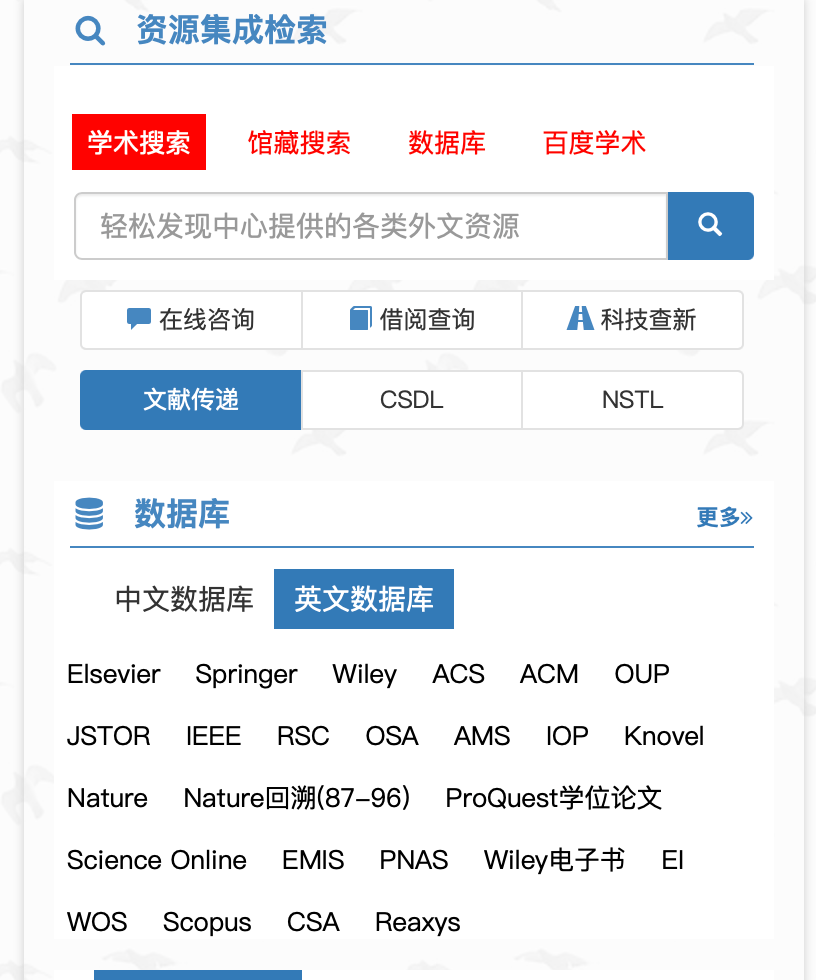
\includegraphics{Fig/ch5/lib1-fs8.png}
\caption{外文数据库}
\end{figure}

\begin{figure}
\centering
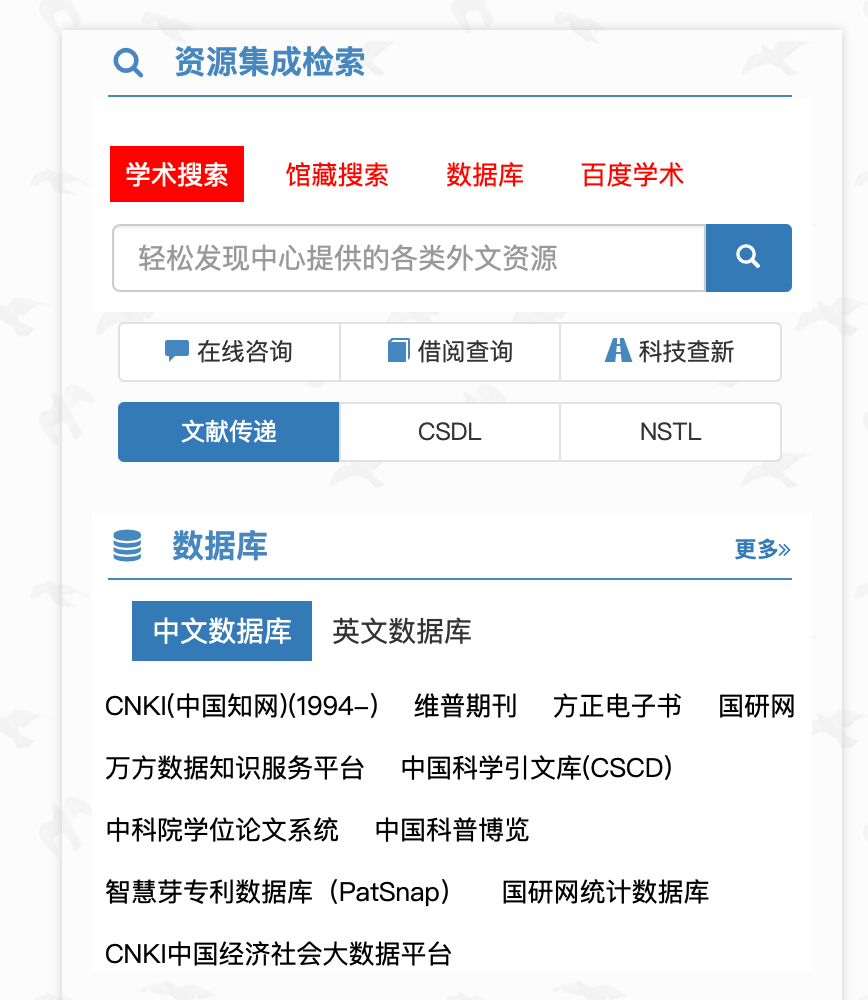
\includegraphics{Fig/ch5/lib2-fs8.png}
\caption{中文数据库}
\end{figure}

\hypertarget{ux6570ux636e}{%
\section{数据}\label{ux6570ux636e}}

绝大部分我们使用的数据已经可以从网上公开渠道获取,利用搜索引擎即可找到下载入口。 很多数据存放于各大数据中心,我们列举一部分常用的数据中心。

\begin{itemize}
\tightlist
\item
  国家冰川冻土沙漠数据中心 \url{http://www.ncdc.ac.cn}
\item
  国家青藏高原科学数据中心 \url{http://www.tpdc.ac.cn}
\item
  资源环境科学与数据中心 \url{https://www.resdc.cn}
\item
  NASA Earth Observation Data \url{https://www.earthdata.nasa.gov}
\item
  USGS EarthExplorer \url{https://earthexplorer.usgs.gov}
\item
  World Climate Research Programme, CMIP6 data \url{https://esgf-node.llnl.gov/projects/cmip6/}
\item
  World Soil Information \url{https://www.isric.org}
\item
  USDA Web Soil Survey \url{https://websoilsurvey.sc.egov.usda.gov/App/HomePage.htm}
\item
  FAO Soil Portal \url{https://www.fao.org/soils-portal/data-hub/soil-maps-and-databases/en/}
\item
  MERIT Hydro: global hydrography datasets \url{http://hydro.iis.u-tokyo.ac.jp/~yamadai/MERIT_Hydro/}
\item
  MERIT-Basins \url{https://www.reachhydro.org/home/params/merit-basins}
\item
  National Hydrography Dataset (NHD) \url{https://www.usgs.gov/national-hydrography/national-hydrography-dataset}
\item
  HydroSHEDS \url{https://www.hydrosheds.org/}
\end{itemize}

\hypertarget{servers}{%
\chapter{计算与存储}\label{servers}}

本研究组分别有三台共组员使用的计算服务器和网络存储.
三台服务器分别为Windows Server远程桌面、Ubuntu远程桌面、多节点高性能计算机群(SHUDHPC)。

各服务器访问IP分别为:

\begin{longtable}[]{@{}
  >{\centering\arraybackslash}p{(\columnwidth - 8\tabcolsep) * \real{0.2143}}
  >{\centering\arraybackslash}p{(\columnwidth - 8\tabcolsep) * \real{0.1429}}
  >{\centering\arraybackslash}p{(\columnwidth - 8\tabcolsep) * \real{0.1905}}
  >{\centering\arraybackslash}p{(\columnwidth - 8\tabcolsep) * \real{0.1905}}
  >{\centering\arraybackslash}p{(\columnwidth - 8\tabcolsep) * \real{0.2619}}@{}}
\toprule\noalign{}
\begin{minipage}[b]{\linewidth}\centering
平台
\end{minipage} & \begin{minipage}[b]{\linewidth}\centering
主机名
\end{minipage} & \begin{minipage}[b]{\linewidth}\centering
公网IP地址
\end{minipage} & \begin{minipage}[b]{\linewidth}\centering
内网IP地址
\end{minipage} & \begin{minipage}[b]{\linewidth}\centering
端口转发地址
\end{minipage} \\
\midrule\noalign{}
\endhead
\bottomrule\noalign{}
\endlastfoot
计算集群 & SHUDHPC & shud.vip(210.77.77.22) & 10.0.1.100 & 210.77.77.25:318xx \\
Ubuntu远程桌面 & uDesk & 210.77.77.23 & 10.0.1.23 & 210.77.77.25:319xx \\
Windows远程桌面 & Win-Desk & 210.77.77.24 & 10.0.1.24 & 210.77.77.25:320xx \\
路由器 & H3C & 210.77.77.25 & 10.0.1.1 & 无 \\
NAS共享网盘 & shudxyz & nas.shud.vip(210.77.77.36) & 10.0.1.26 & 无 \\
\end{longtable}

\textbf{注意}:ssh登录端口统一为32099

\textbf{SHUDHPC与uDesk通过NIS共享同一套账户系统,因此,在SHUDHPC和uDesk上面的登录账户和用户主目录完全相同;uDesk上支持Linux图形桌面,方便用户进行可视化操作。}

\begin{figure}
\centering
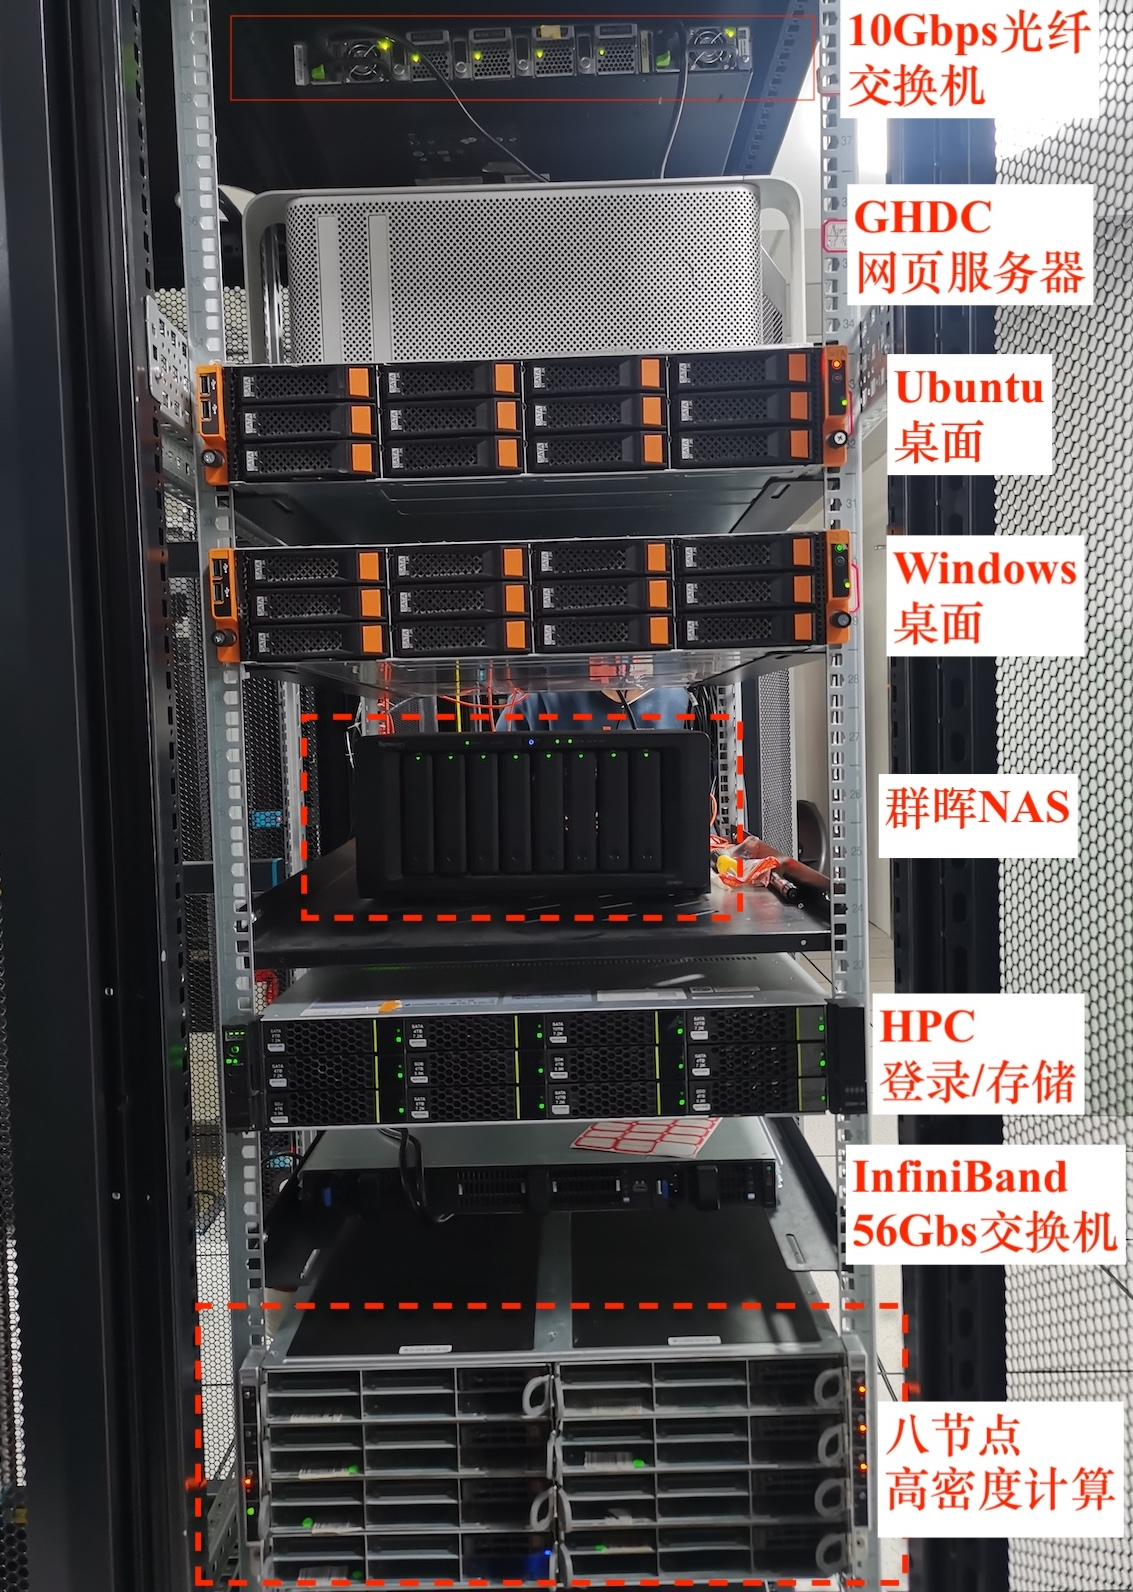
\includegraphics{Fig/ch5/machine.jpeg}
\caption{所有主机照片}
\end{figure}

\hypertarget{nasux7f51ux7edcux5b58ux50a8}{%
\section{NAS网络存储}\label{nasux7f51ux7edcux5b58ux50a8}}

本组使用群辉DS1821+建设了100TB的网络存储空间,供组内成员和合作者使用。

Synology Drive是依托本组的NAS网络存储建设的,可以远程以网络磁盘的方式访问,也可以使用sftp,、Synology Drive、rsync、SMB、AFP、NFS等方式访问。

\hypertarget{ux8d26ux53f7ux5f00ux901aux6ce8ux9500}{%
\subsection{账号开通/注销}\label{ux8d26ux53f7ux5f00ux901aux6ce8ux9500}}

\begin{itemize}
\item
  \textbf{账号开通}

  \begin{itemize}
  \tightlist
  \item
    在加入本组后,向PI报告你的邮箱;由PI给你开通账号,并告知用户名和密码。
  \item
    账号的权限等级由个人身份决定,不同权限对NAS的读写权限略有不同。
  \item
    账号开通后,你会收到一封邮件,邮件包含了NAS服务的访问地址。请在收到邮件后登录NAS页面,并修改秘密。
  \end{itemize}
\item
  \textbf{账号注销}

  \begin{itemize}
  \tightlist
  \item
    成员离开本组后,账号会继续保留至少一年。
  \item
    你可以在一年内,备份个人网盘内的数据。一年后,你的账号将被删除,无法再访问NAS系统。
  \end{itemize}
\end{itemize}

\hypertarget{nasux6587ux4ef6ux7ed3ux6784}{%
\subsection{NAS文件结构}\label{nasux6587ux4ef6ux7ed3ux6784}}

当前的NAS文件结构与读写权限见下图:

\begin{figure}
\centering
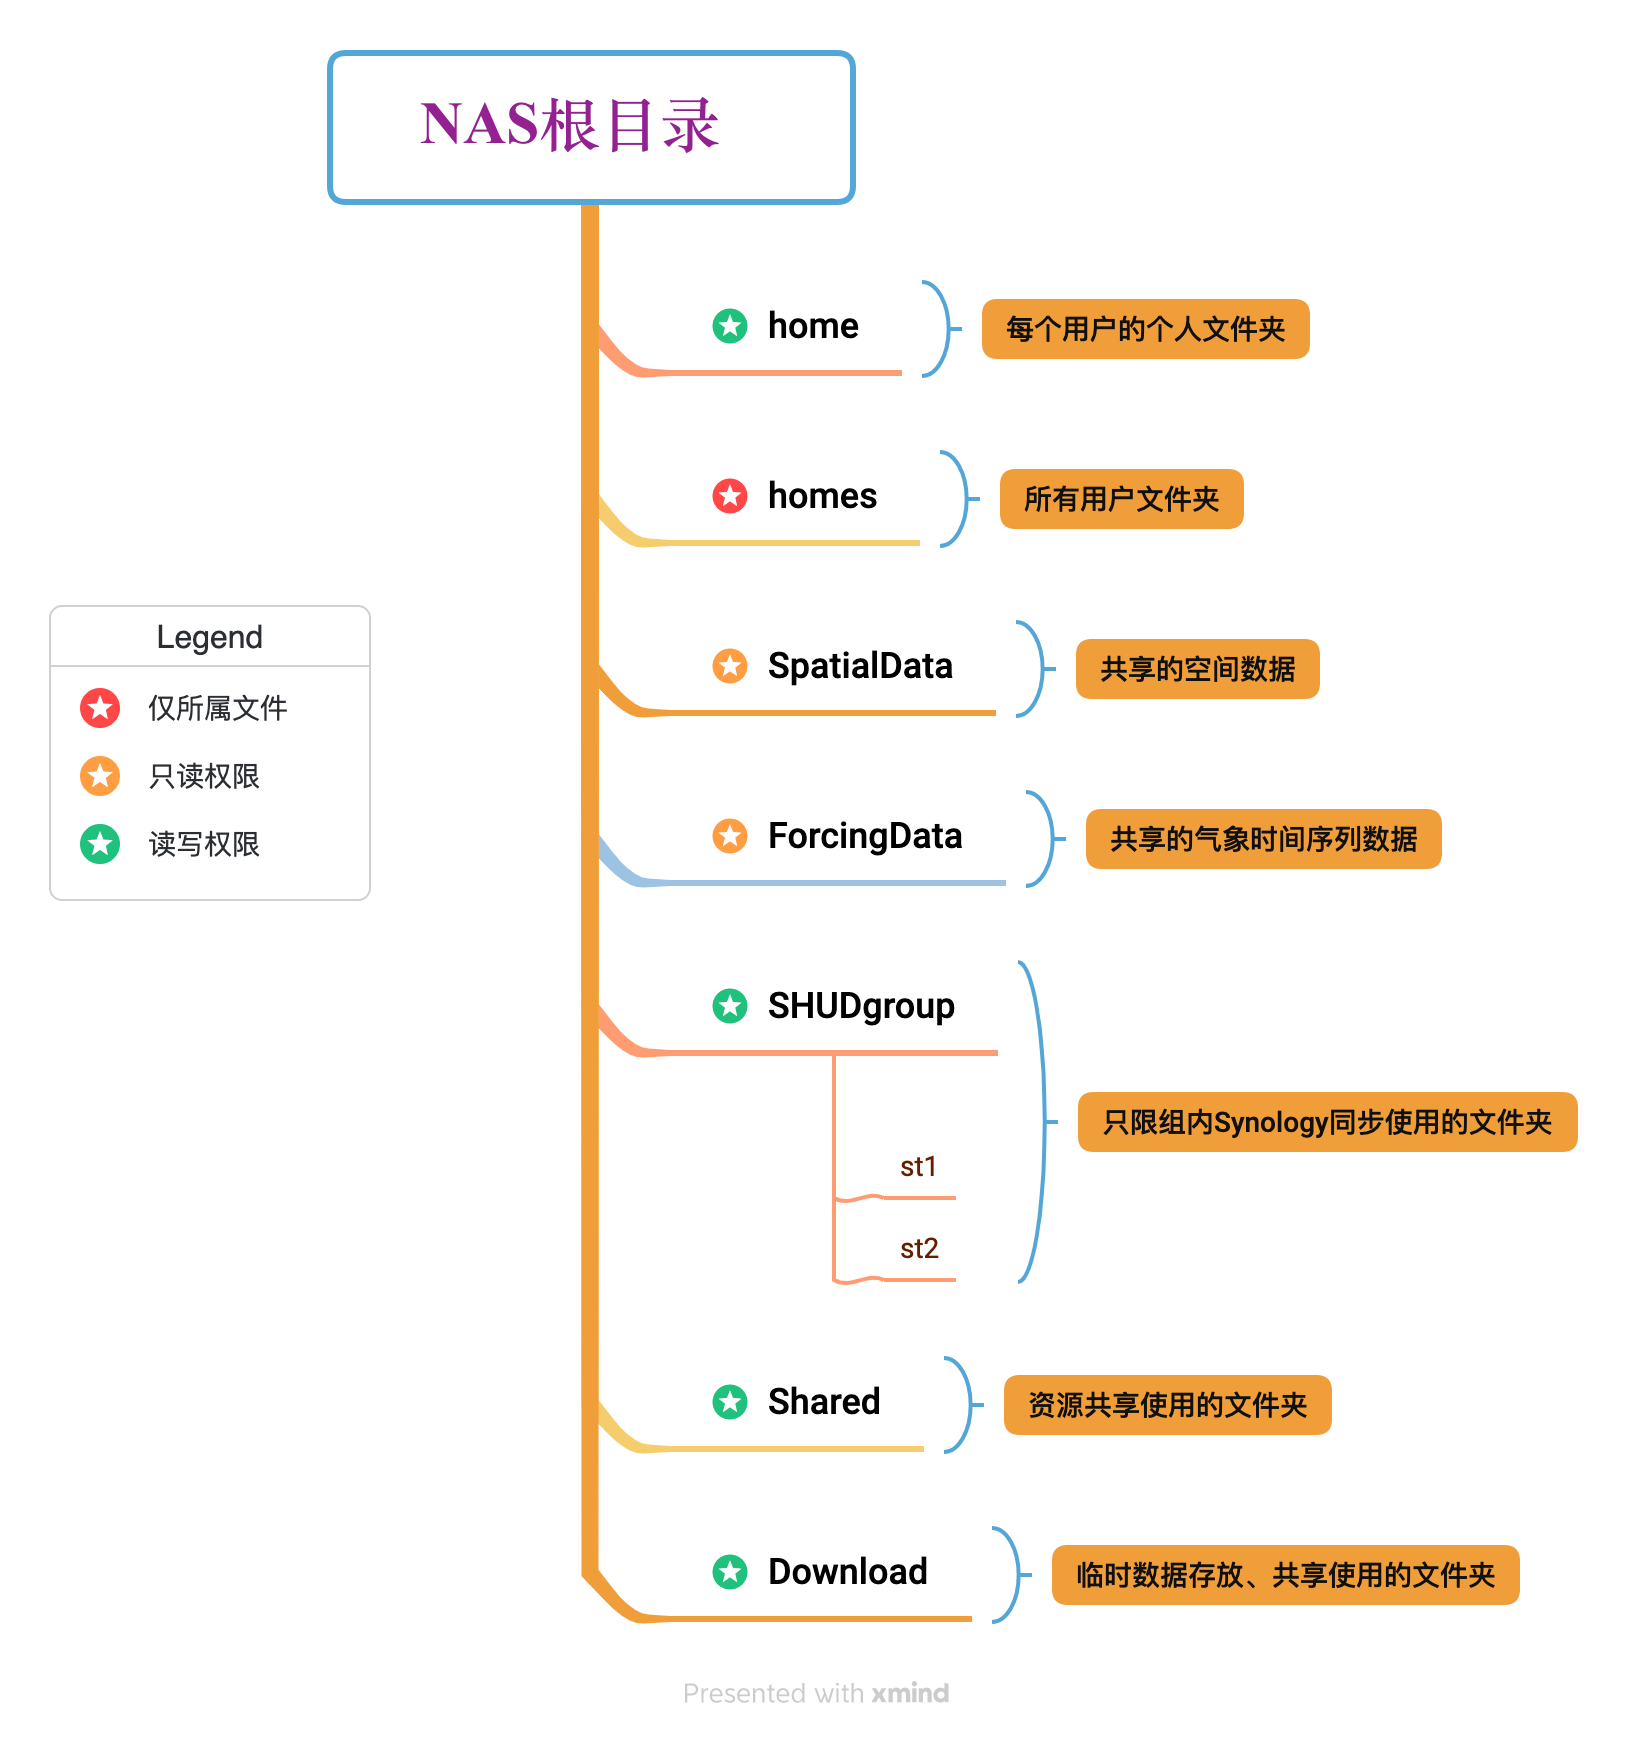
\includegraphics{Fig/ch5/nas_structure.png}
\caption{NAS上的文件结构与权限}
\end{figure}

更具体的信息见下表:

\begin{longtable}[]{@{}
  >{\centering\arraybackslash}p{(\columnwidth - 8\tabcolsep) * \real{0.1471}}
  >{\centering\arraybackslash}p{(\columnwidth - 8\tabcolsep) * \real{0.1471}}
  >{\centering\arraybackslash}p{(\columnwidth - 8\tabcolsep) * \real{0.1471}}
  >{\centering\arraybackslash}p{(\columnwidth - 8\tabcolsep) * \real{0.1471}}
  >{\raggedright\arraybackslash}p{(\columnwidth - 8\tabcolsep) * \real{0.4118}}@{}}
\toprule\noalign{}
\begin{minipage}[b]{\linewidth}\centering
文件夹
\end{minipage} & \begin{minipage}[b]{\linewidth}\centering
学生权限
\end{minipage} & \begin{minipage}[b]{\linewidth}\centering
合作者权限
\end{minipage} & \begin{minipage}[b]{\linewidth}\centering
容量
\end{minipage} & \begin{minipage}[b]{\linewidth}\raggedright
\textbf{注意事项}
\end{minipage} \\
\midrule\noalign{}
\endhead
\bottomrule\noalign{}
\endlastfoot
homes & 无 & 无 & 无限 & 所有用户文件都存放于此,普通用户无法访问 \\
home & 读写 & 读写 & 10TB & 用户个人主目录,其他用户无法访问 \\
SpatialData & 只读 & 只读 & 10TB & 仅特定用户有权更新 \\
ForcingData & 只读 & 只读 & 10TB & 仅特定用户有权更新 \\
SHUDgroup & 读写 & 读写 & 10TB & 组内成员间自动同步。勿随意存放文件 \\
Shared & 读写 & 读写 & 10TB & 共享资源 \\
Download & 读写 & 读写 & 无限 & 文件临时存放。所有人可写,勿长期存放重要文件 \\
Baomi & 无 & 无 & 无限 & 保密数据,仅在特殊需要时共享给指定用户 \\
\end{longtable}

\hypertarget{ux8bbfux95eenas}{%
\subsection{访问NAS}\label{ux8bbfux95eenas}}

\begin{itemize}
\tightlist
\item
  NAS名称: shudxyz
\item
  NAS访问地址: \url{https://nas.shud.vip} 或者 \url{https://nas.shud.vip}
\item
  用户名:username{[}默认为姓名全拼{]}
\item
  密码: {[}随机密码,请查看邮件{]}
\end{itemize}

\hypertarget{nas-ux4f5cux4e3aux7f51ux7edcux78c1ux76d8}{%
\subsection{NAS 作为网络磁盘}\label{nas-ux4f5cux4e3aux7f51ux7edcux78c1ux76d8}}

\begin{itemize}
\item
  Mac OS

  \begin{itemize}
  \tightlist
  \item
    打开Finder(访达),然后使用键盘CMD+k,访问网络地址。
  \item
    在打开的窗口中输入:\texttt{afp://nas.shud.vip}或者\texttt{afp://210.77.77.36}。然后点击\texttt{连接(Connect)}
  \item
    然后提示框要求输入\texttt{用户名和密码}。
  \item
    选择你需要加载的磁盘。
  \end{itemize}
\item
  Windows

  \begin{enumerate}
  \def\labelenumi{\arabic{enumi}.}
  \tightlist
  \item
    打开文件管理器,找到\texttt{映射网络磁盘(Map\ network\ driver)},
  \end{enumerate}

  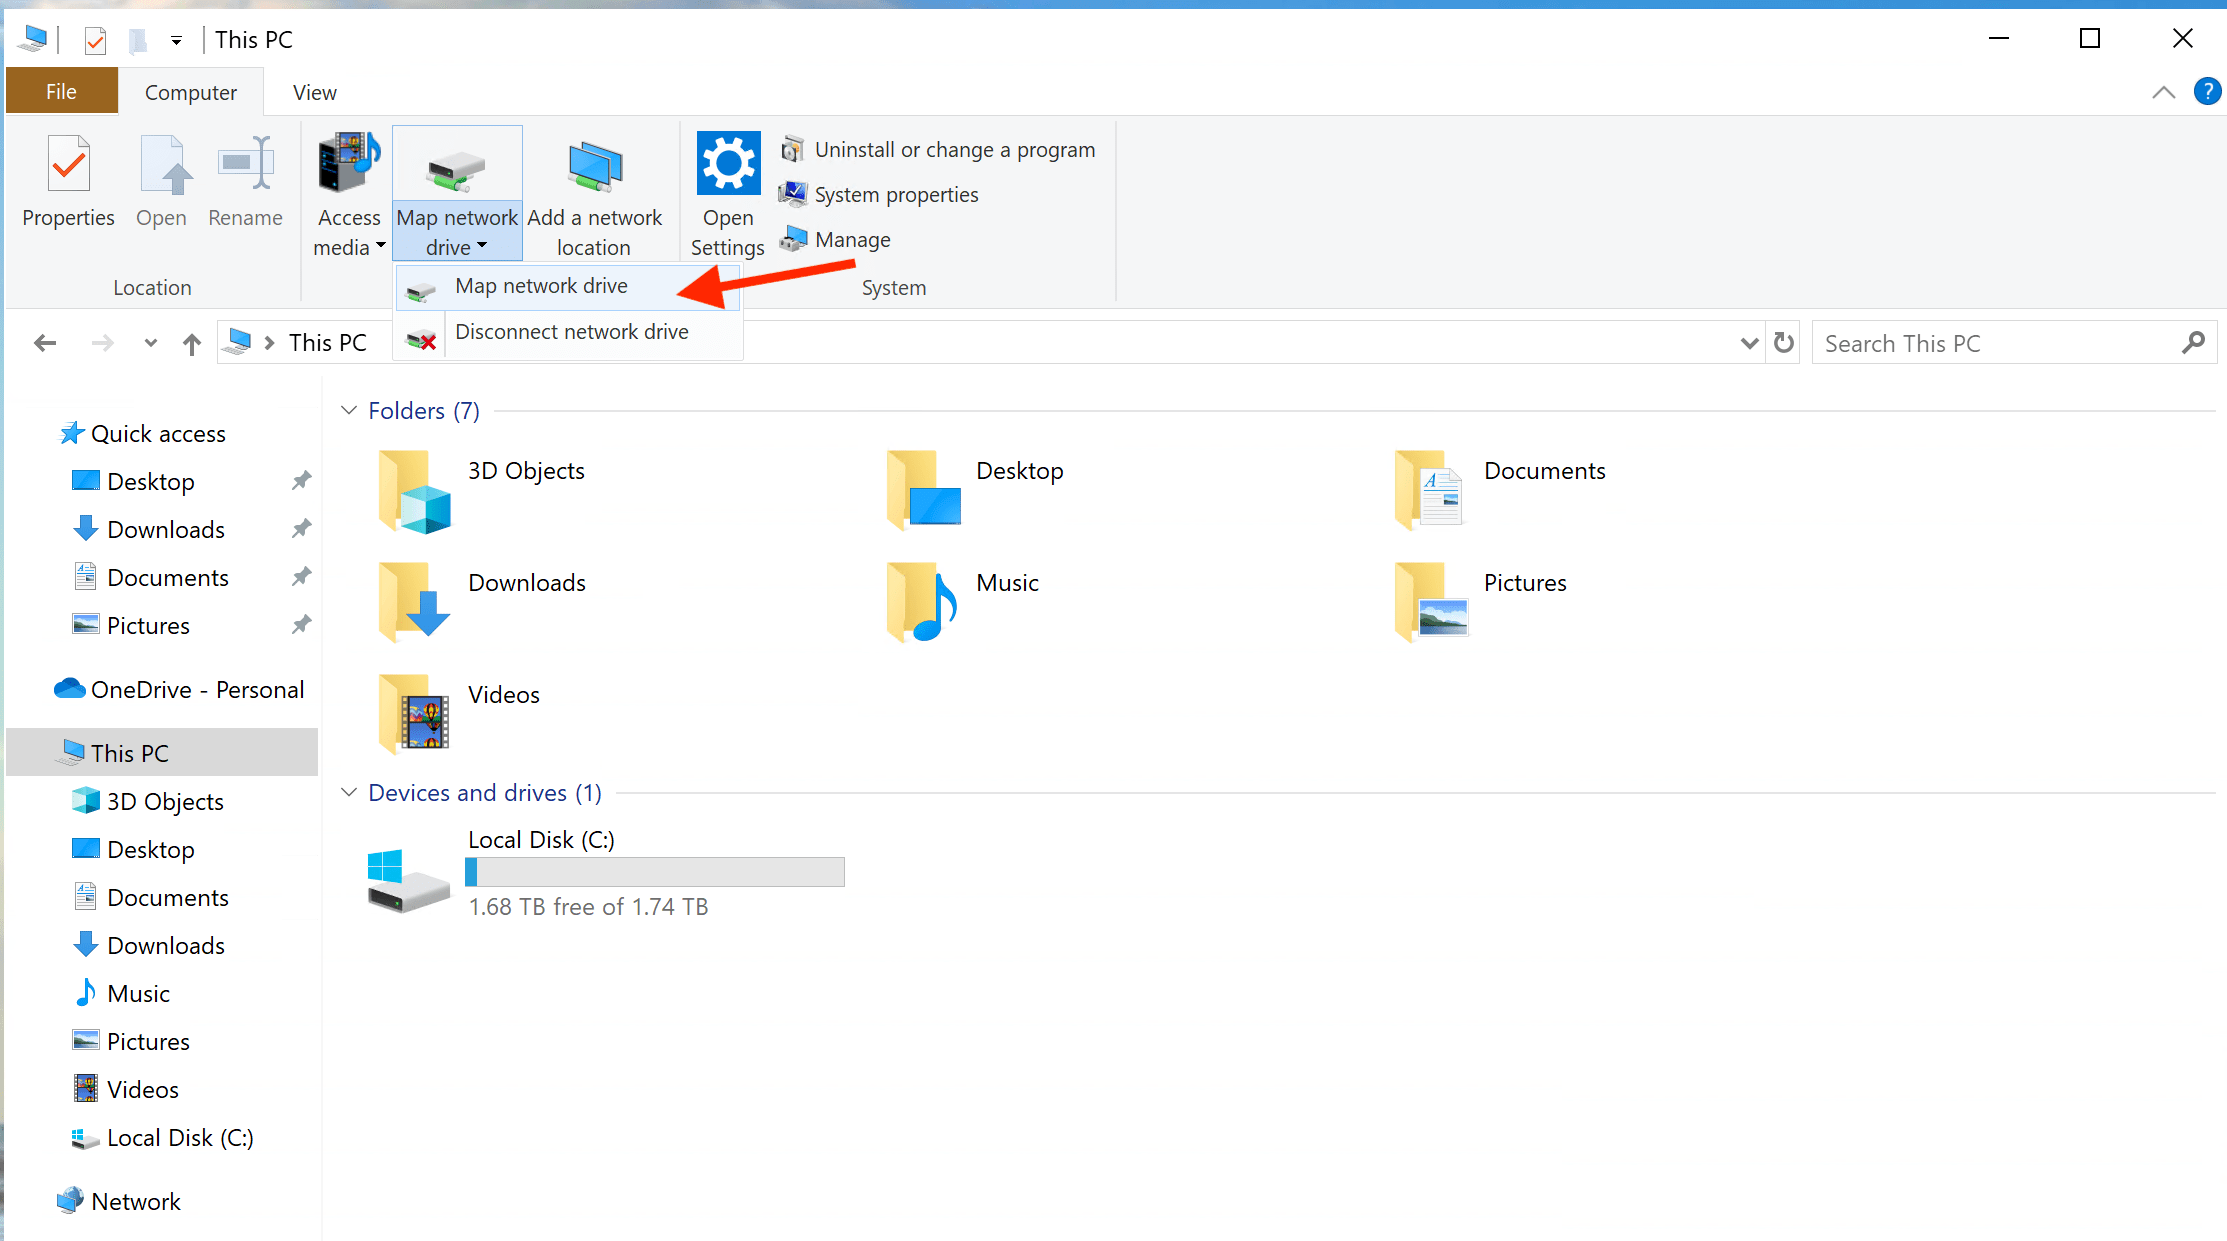
\includegraphics{Fig/ch5/win_mapdisk-1.png}

  \begin{enumerate}
  \def\labelenumi{\arabic{enumi}.}
  \tightlist
  \item
    在打开的窗口中输入需要加载的\texttt{磁盘IP和路径},例如\texttt{\textbackslash{}\textbackslash{}nas.shud.vip\textbackslash{}home}或者\texttt{\textbackslash{}\textbackslash{}nas.shud.vip\textbackslash{}ForcingData}。点击\texttt{完成}
  \end{enumerate}

  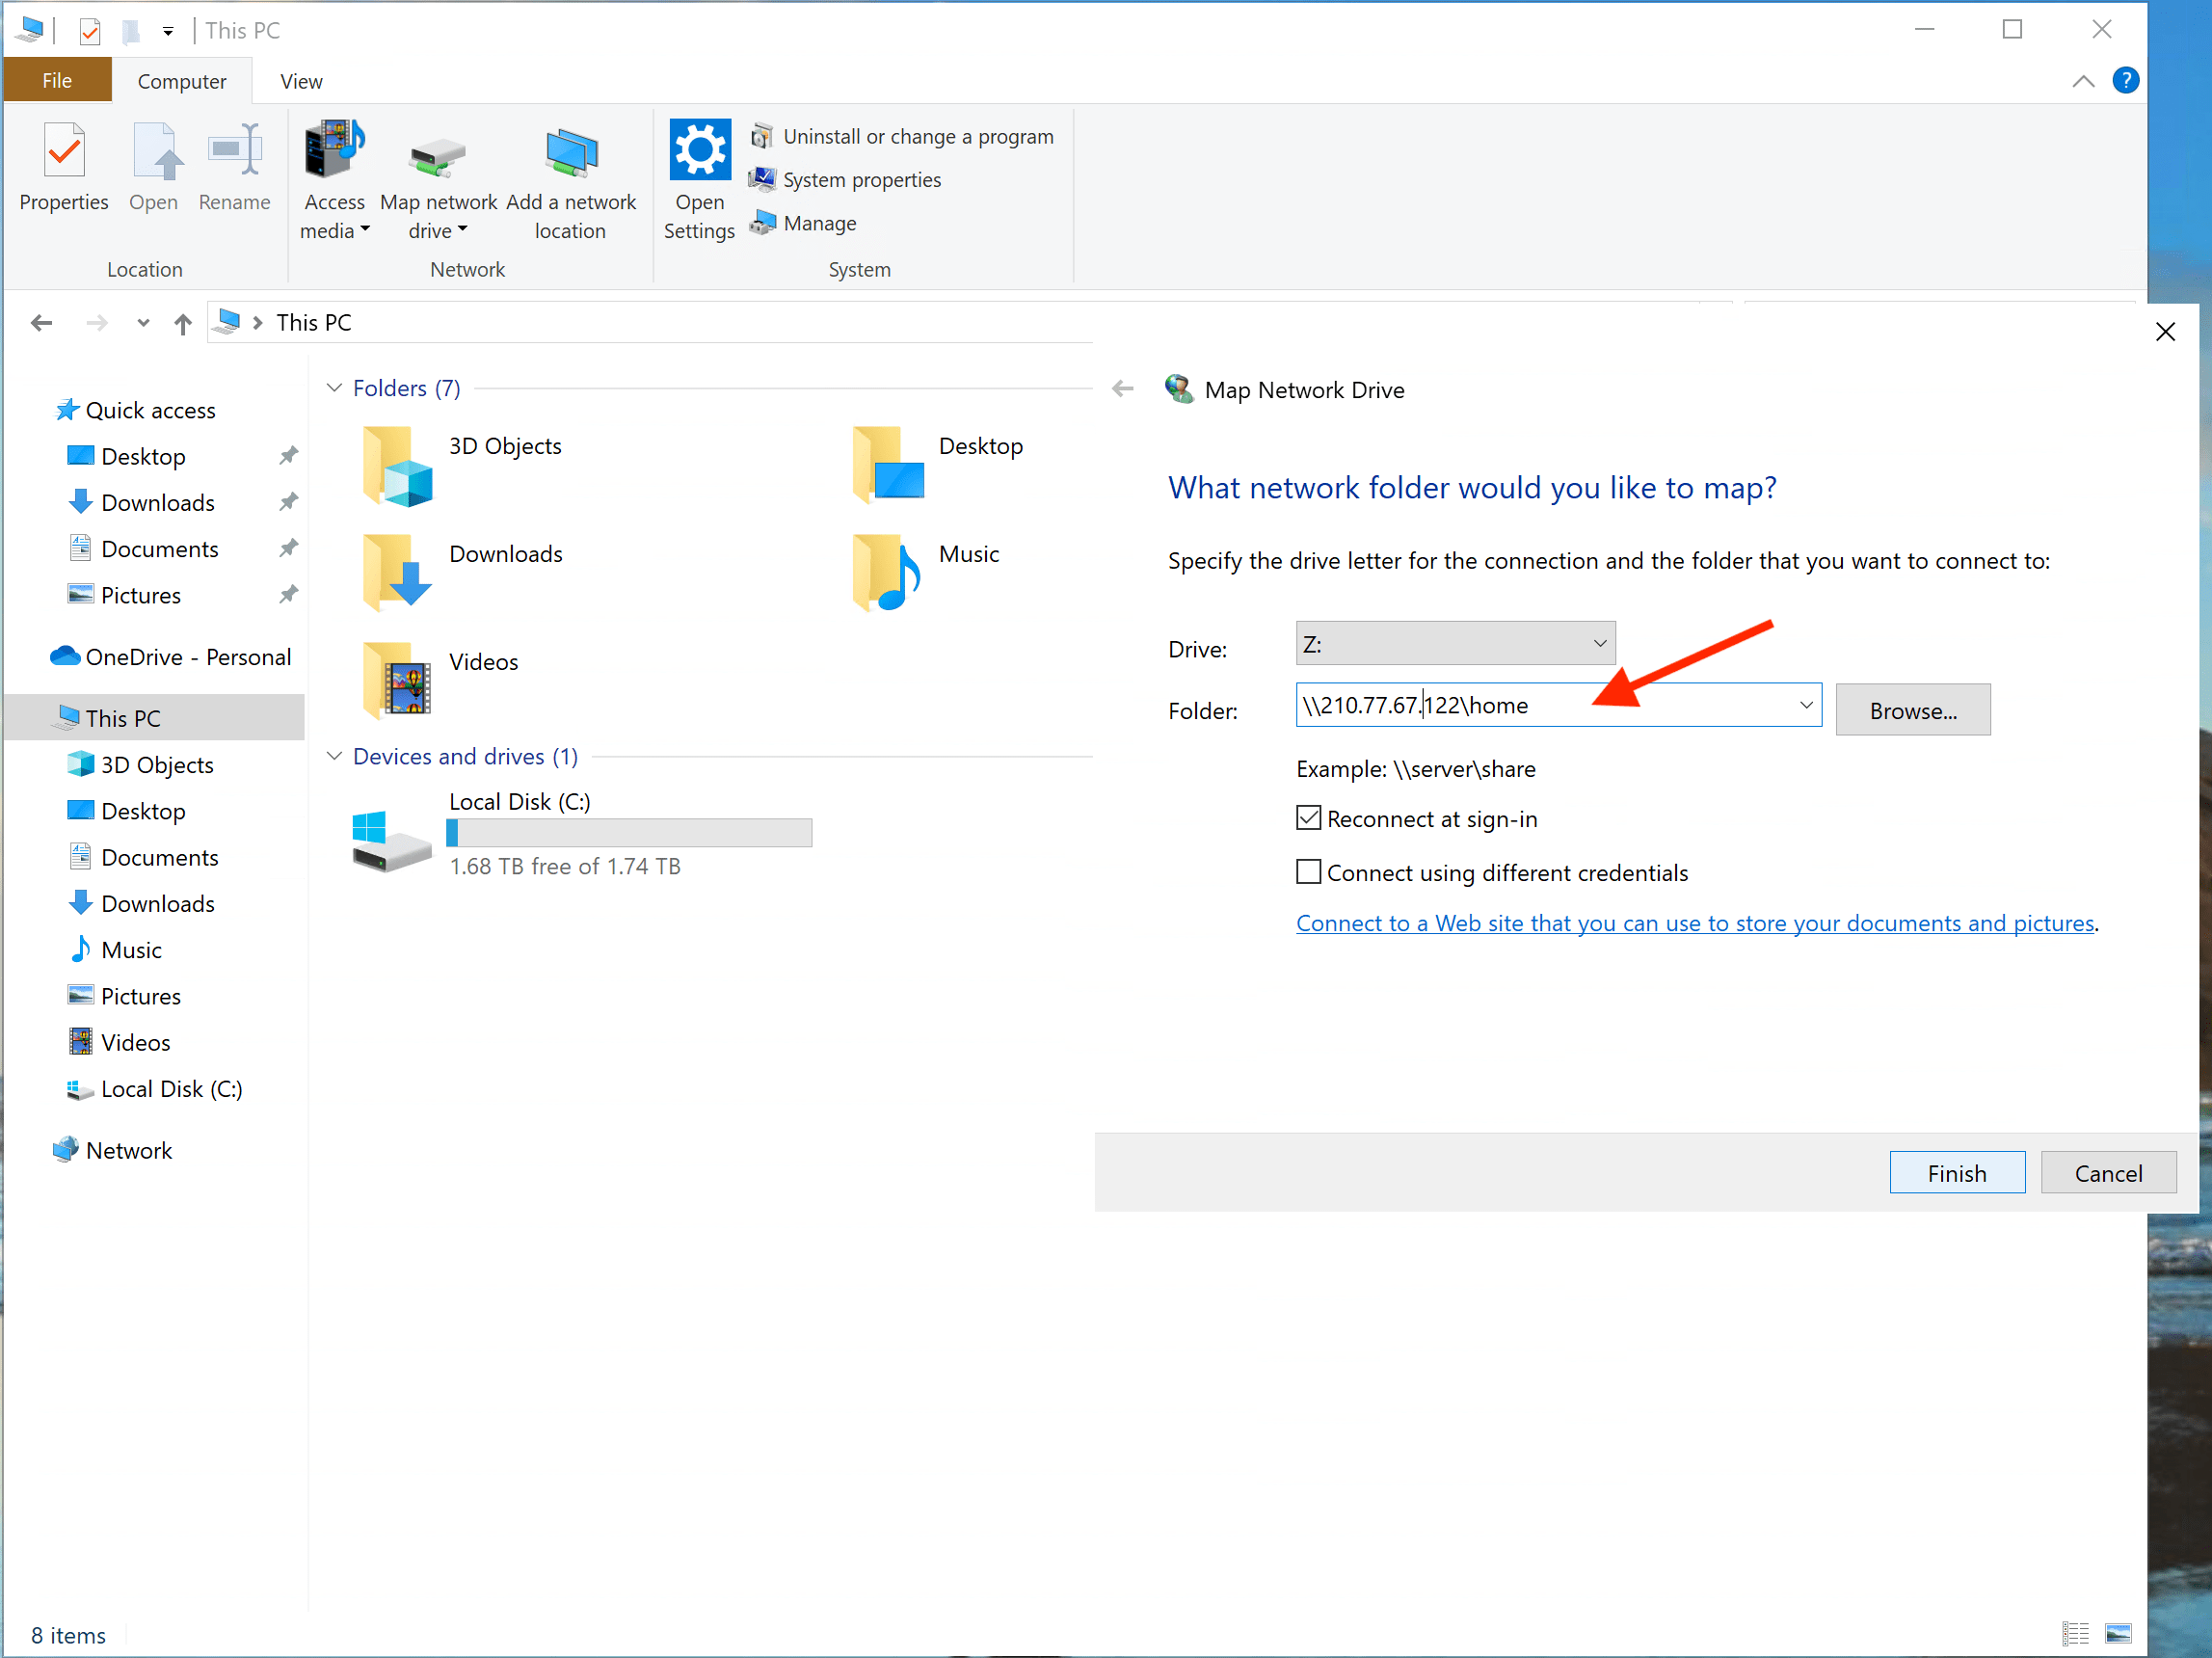
\includegraphics{Fig/ch5/win_mapdisk-2.png}

  \begin{enumerate}
  \def\labelenumi{\arabic{enumi}.}
  \tightlist
  \item
    根据提示框输入登录NAS使用的\texttt{用户名与密码}。点击\texttt{OK}
  \end{enumerate}

  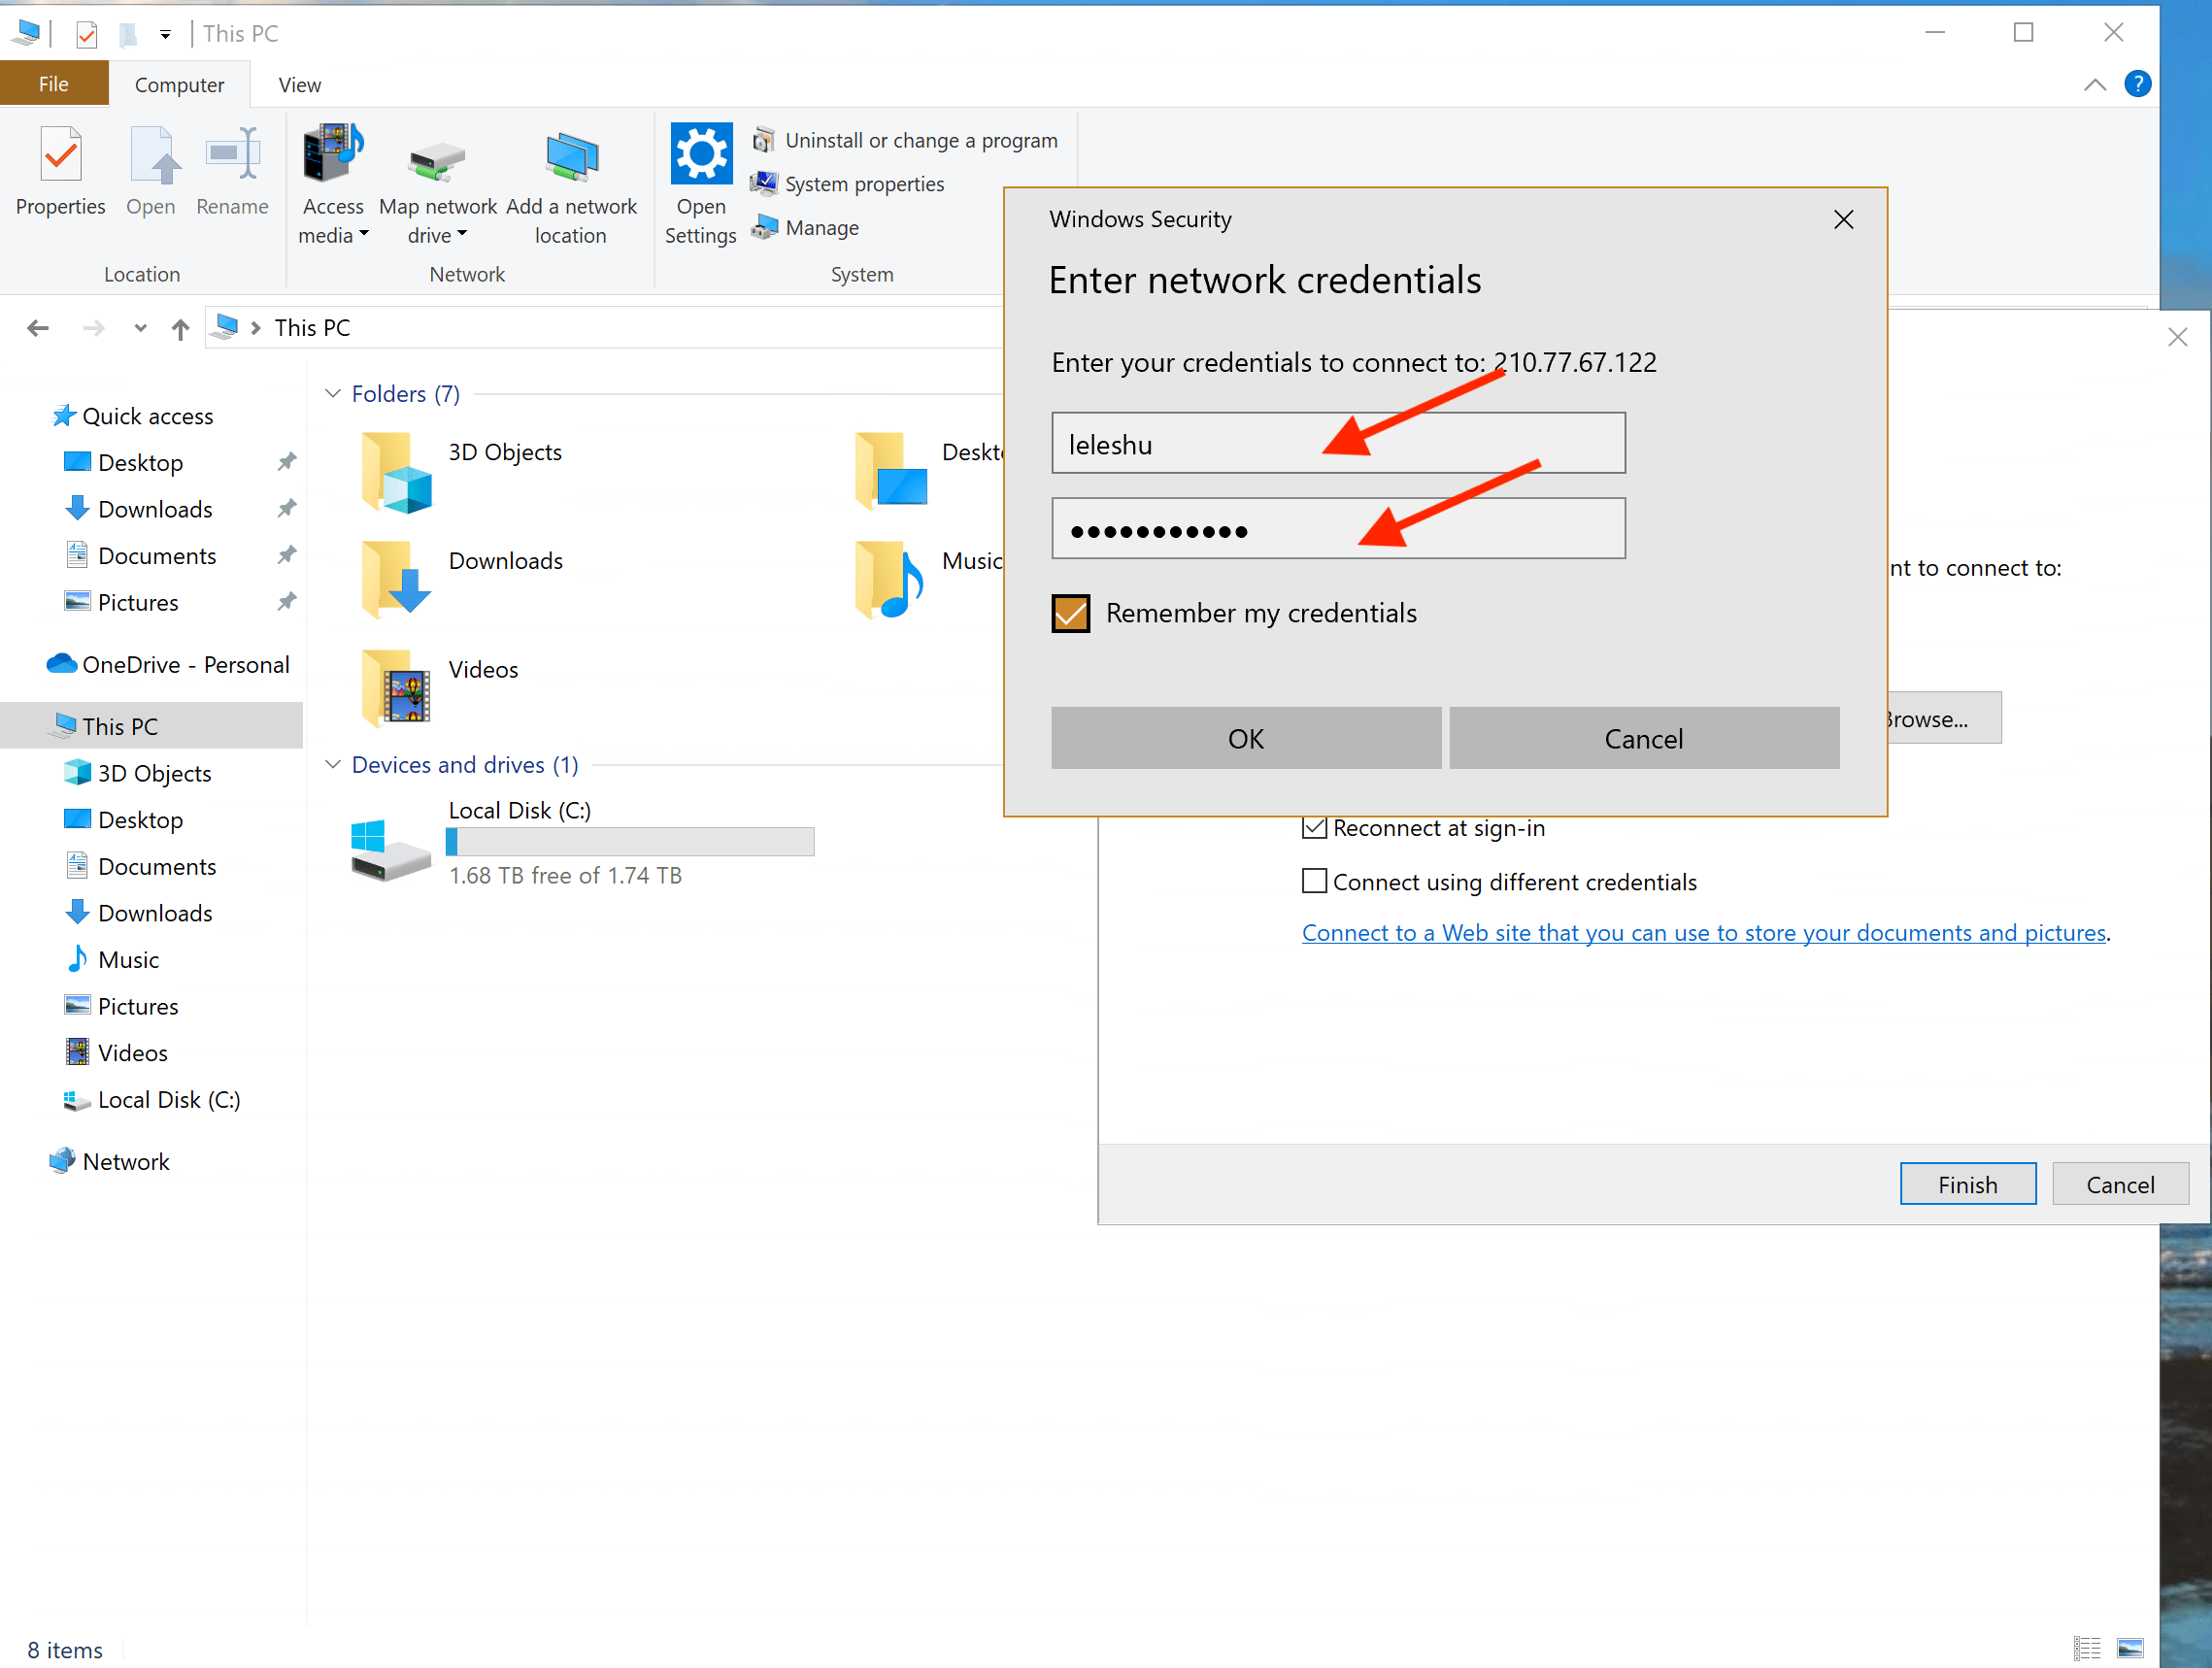
\includegraphics{Fig/ch5/win_mapdisk-3.png}

  \begin{enumerate}
  \def\labelenumi{\arabic{enumi}.}
  \tightlist
  \item
    然后系统会加载指定的网络磁盘,映射其为本地磁盘。此后该网络磁盘将可以像一般本地磁盘一样操作。
  \end{enumerate}

  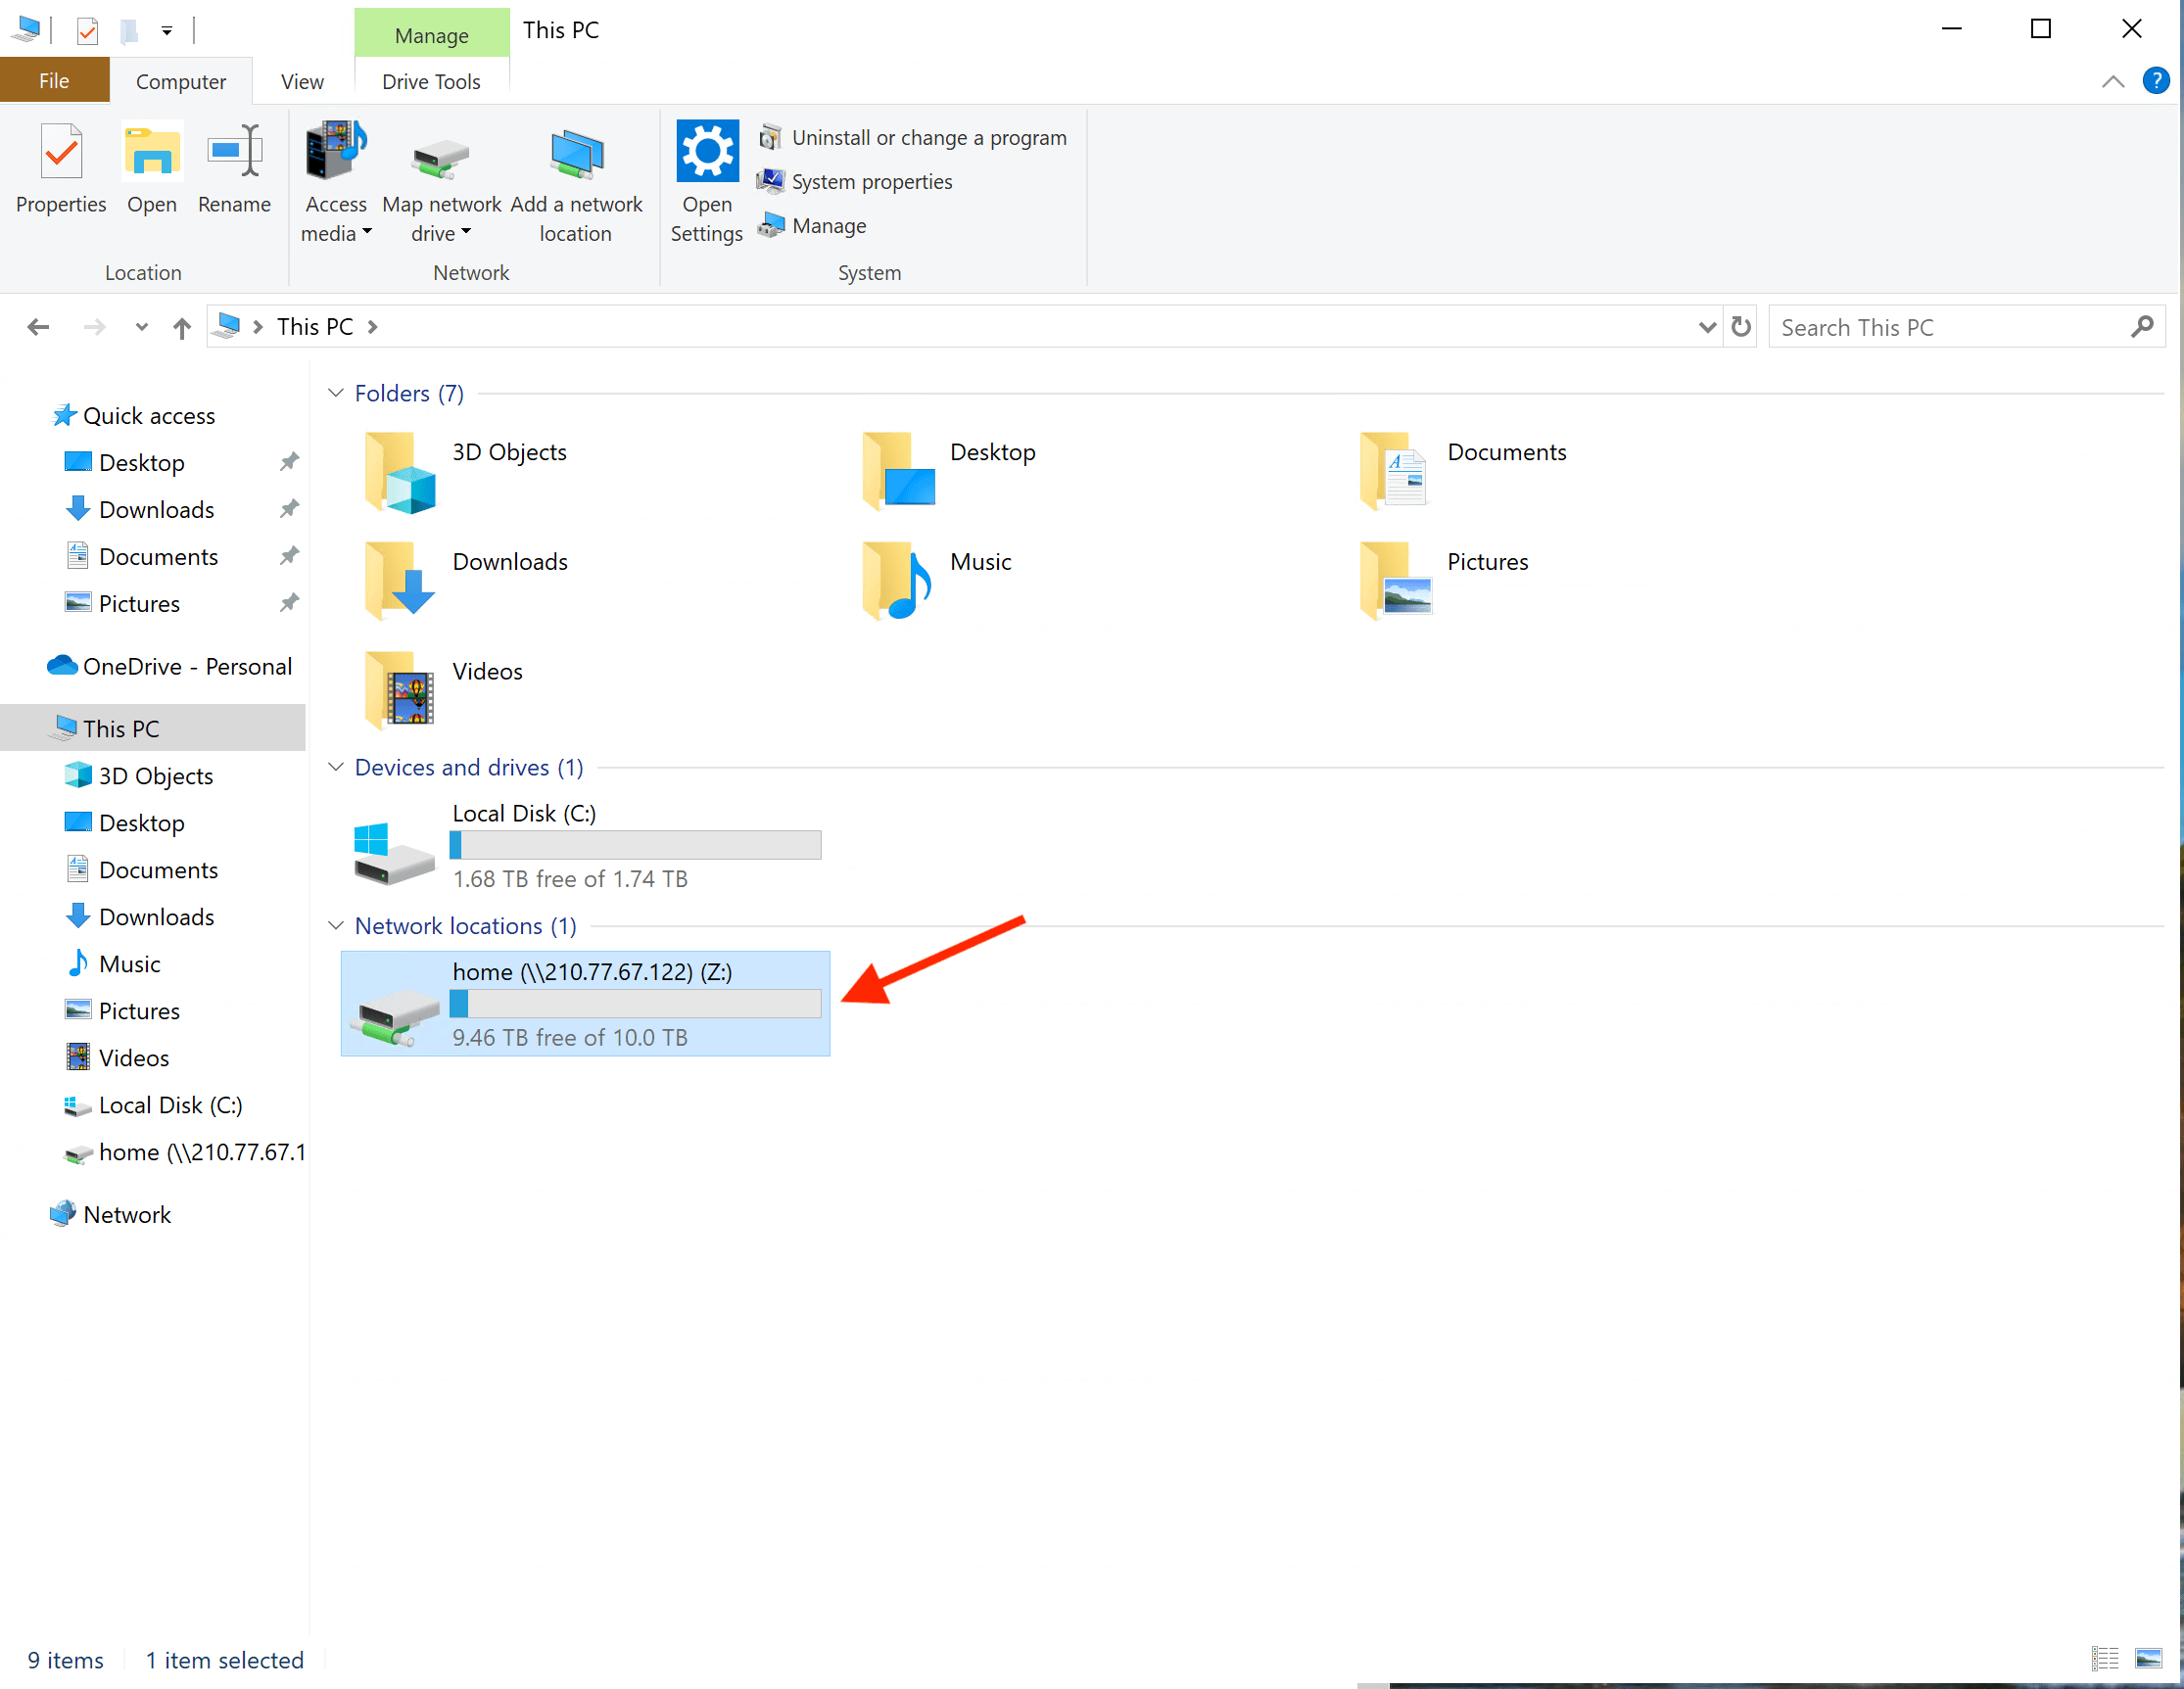
\includegraphics{Fig/ch5/win_mapdisk-4.png}
\end{itemize}

\textbf{注}:如果在Windows远程桌面(Win-Desk)上加载NAS,使用本地IP(\texttt{10.0.1.x}段),可以显著提高网络磁盘的读写速度。

\hypertarget{synology}{%
\subsection{云盘Synology Drive}\label{synology}}

这应该是进入本组第一个学会的软件。软件的安装使用都非常简单,但是你需要学会的是重新思考:

\begin{itemize}
\tightlist
\item
  如何组织自己的文件?
\item
  如何高效的定位自己的文件?
\end{itemize}

加入本组的工作全部在Synology Drive上进行同步。同步文件夹的内容仅自己可以看到,其他用户看不到。
文件备份在NAS云端,任何地点任何电脑上都可以查看/编辑你云盘里面的文件,不会出现\emph{``电脑坏了,文件丢失''},\emph{``文件染病毒打不开''},\emph{``电脑忘记带了,没法交作业''}的情况。

\textbf{注意}:Synology Drive使用中有\texttt{同步(sync)}和\texttt{备份(backup)}两种模式,建议一定要使用\texttt{同步模式},保证自己每一次保存的文件都实时同步在云端。 是否启用备份模式,可以自行选择。

\hypertarget{windowsux8fdcux7a0bux684cux9762}{%
\section{Windows远程桌面}\label{windowsux8fdcux7a0bux684cux9762}}

服务器硬件配置

\begin{longtable}[]{@{}cccc@{}}
\toprule\noalign{}
类别 & 配件 & 参数 & 备注 \\
\midrule\noalign{}
\endhead
\bottomrule\noalign{}
\endlastfoot
平台 & 浪潮雷神SA5212 H5 & 12盘位2U机架式服务器 & \\
CPU & 至强Xeon 金牌 6133 & 每CPU 20核40线程,2.5GHz & 双CPU \\
内存 & 192GB & DDR4 2666Mhz, 12x 16GB & 6通道内存,12条 \\
硬盘 & U.2 NVME & 2TB & \\
网卡 & & 10Gbps 光口 & \\
\end{longtable}

\hypertarget{ux64cdux4f5cux7cfbux7edfux4e0eux8f6fux4ef6}{%
\subsection{操作系统与软件}\label{ux64cdux4f5cux7cfbux7edfux4e0eux8f6fux4ef6}}

\begin{itemize}
\tightlist
\item
  操作系统:Windows Server 2019, 支持远程GUI登录。
\item
  Office: Microsoft Office 365
\item
  文本编辑器:Notepad++, vim.
\item
  PS工具: GIMP
\item
  GIS软件:ArcGIS, QGIS
\item
  编程:Visual Studio Code
\item
  R:R, Rstudio
\item
  计算:Octave
\end{itemize}

\begin{figure}
\centering
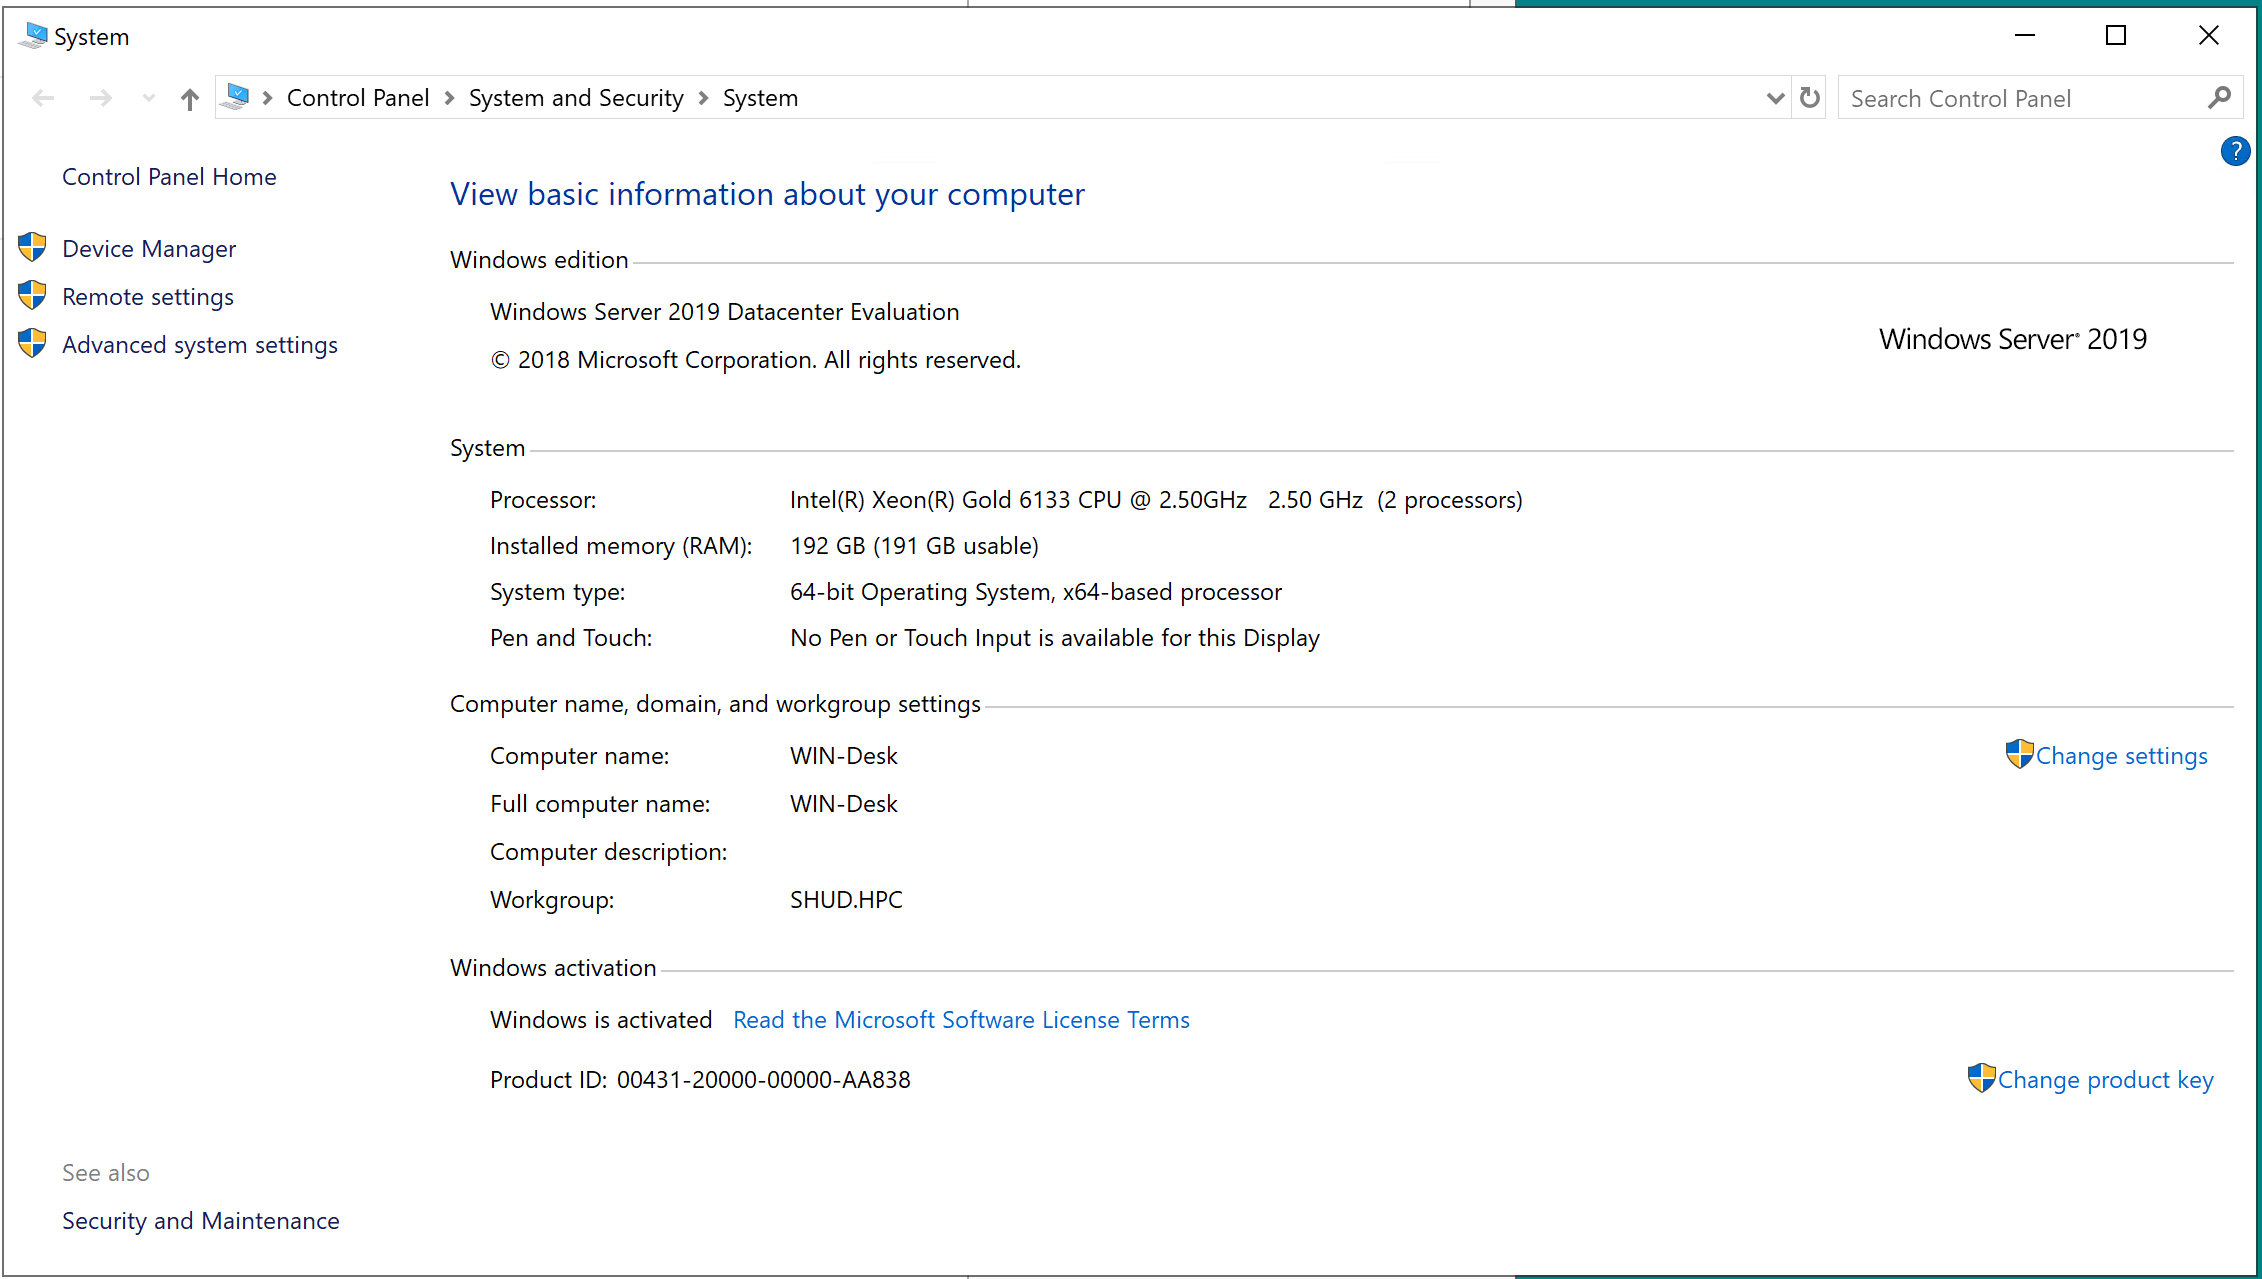
\includegraphics{Fig/ch5/host_win.png}
\caption{Windows系统基本信息}
\end{figure}

\hypertarget{ux767bux5f55ux65b9ux5f0f}{%
\subsection{登录方式}\label{ux767bux5f55ux65b9ux5f0f}}

\begin{itemize}
\tightlist
\item
  软件:Microsoft Remote Desktop
\item
  登录IP: 210.77.77.24
\item
  端口: 默认
\item
  转发IP: 210.77.77.25
\item
  转发端口: 31810
\end{itemize}

\begin{figure}
\centering
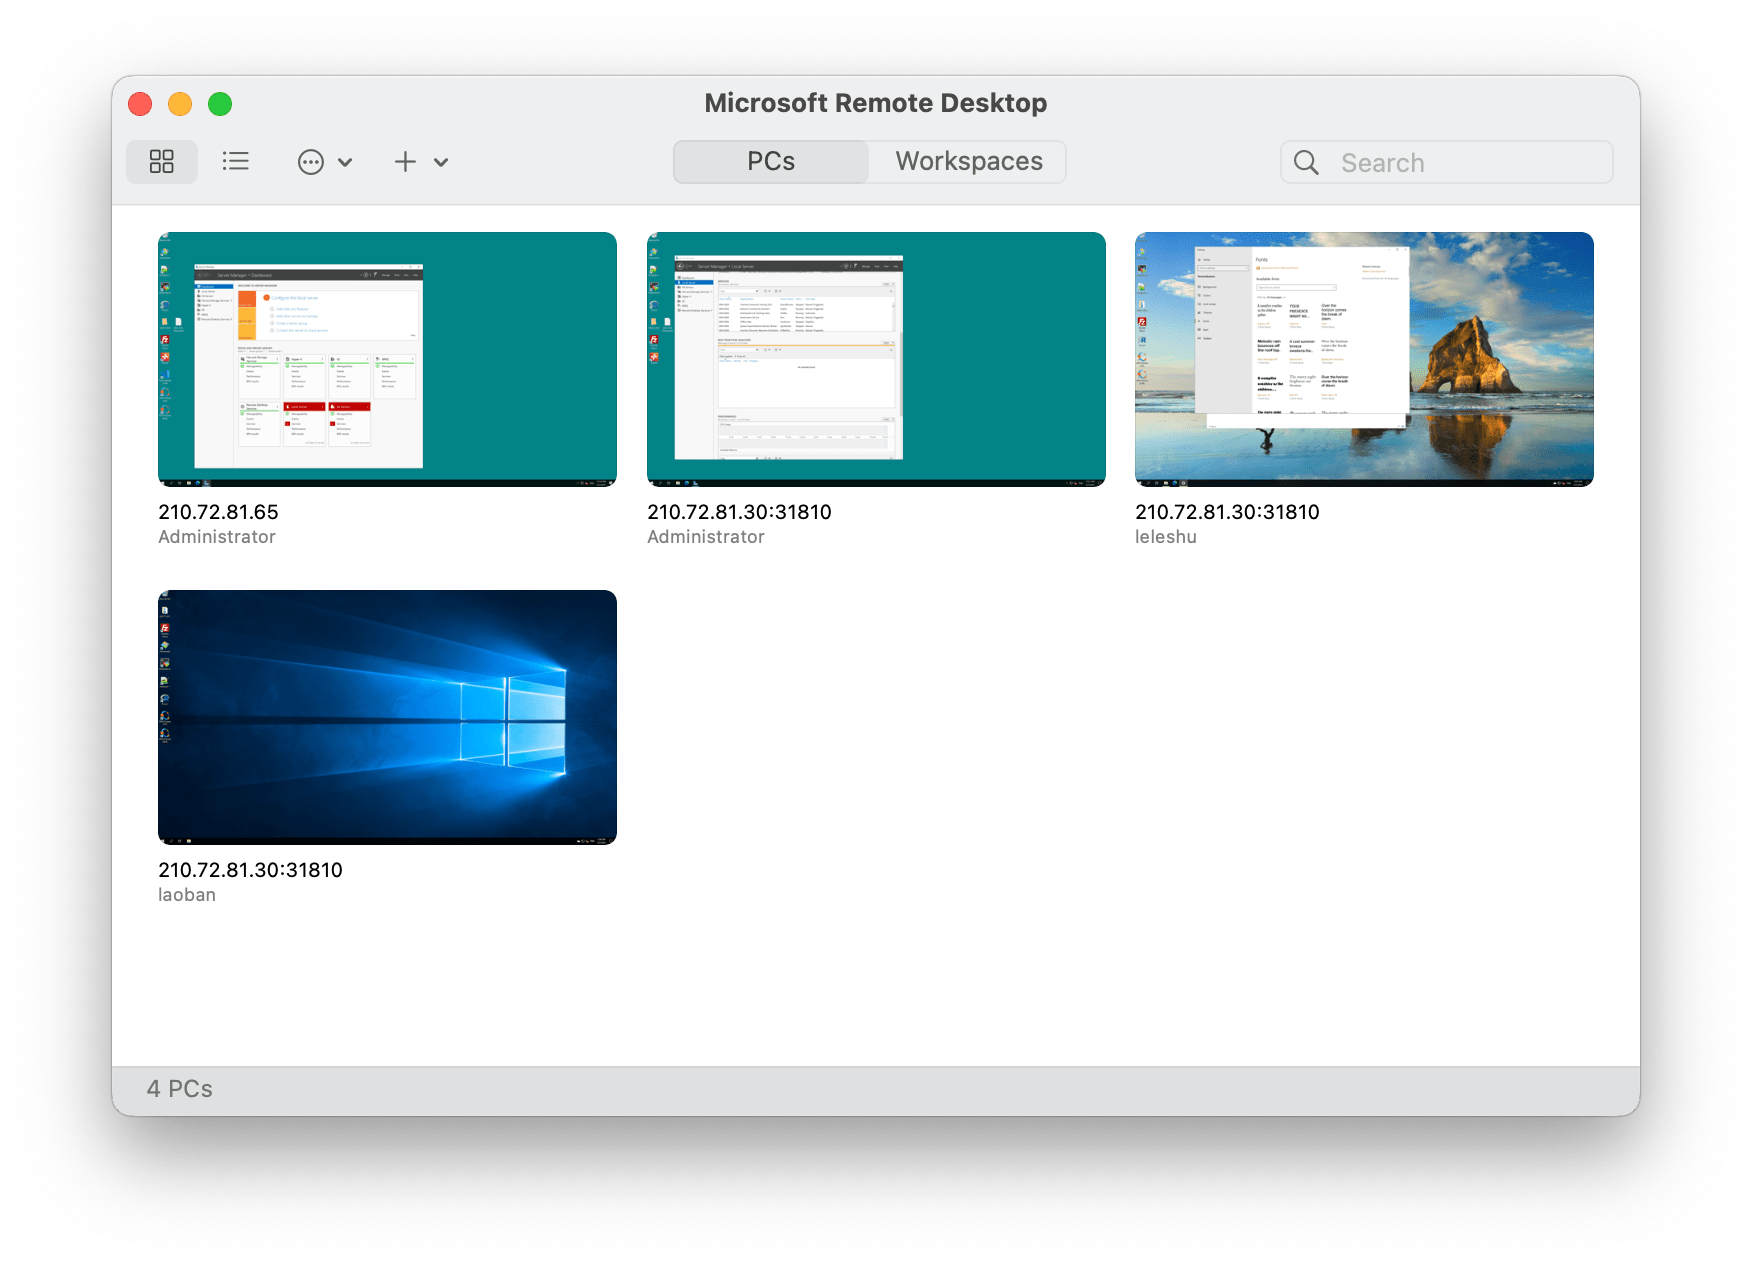
\includegraphics{Fig/ch5/rdp-1.png}
\caption{Microsoft Remote Desktop界面}
\end{figure}

\begin{figure}
\centering
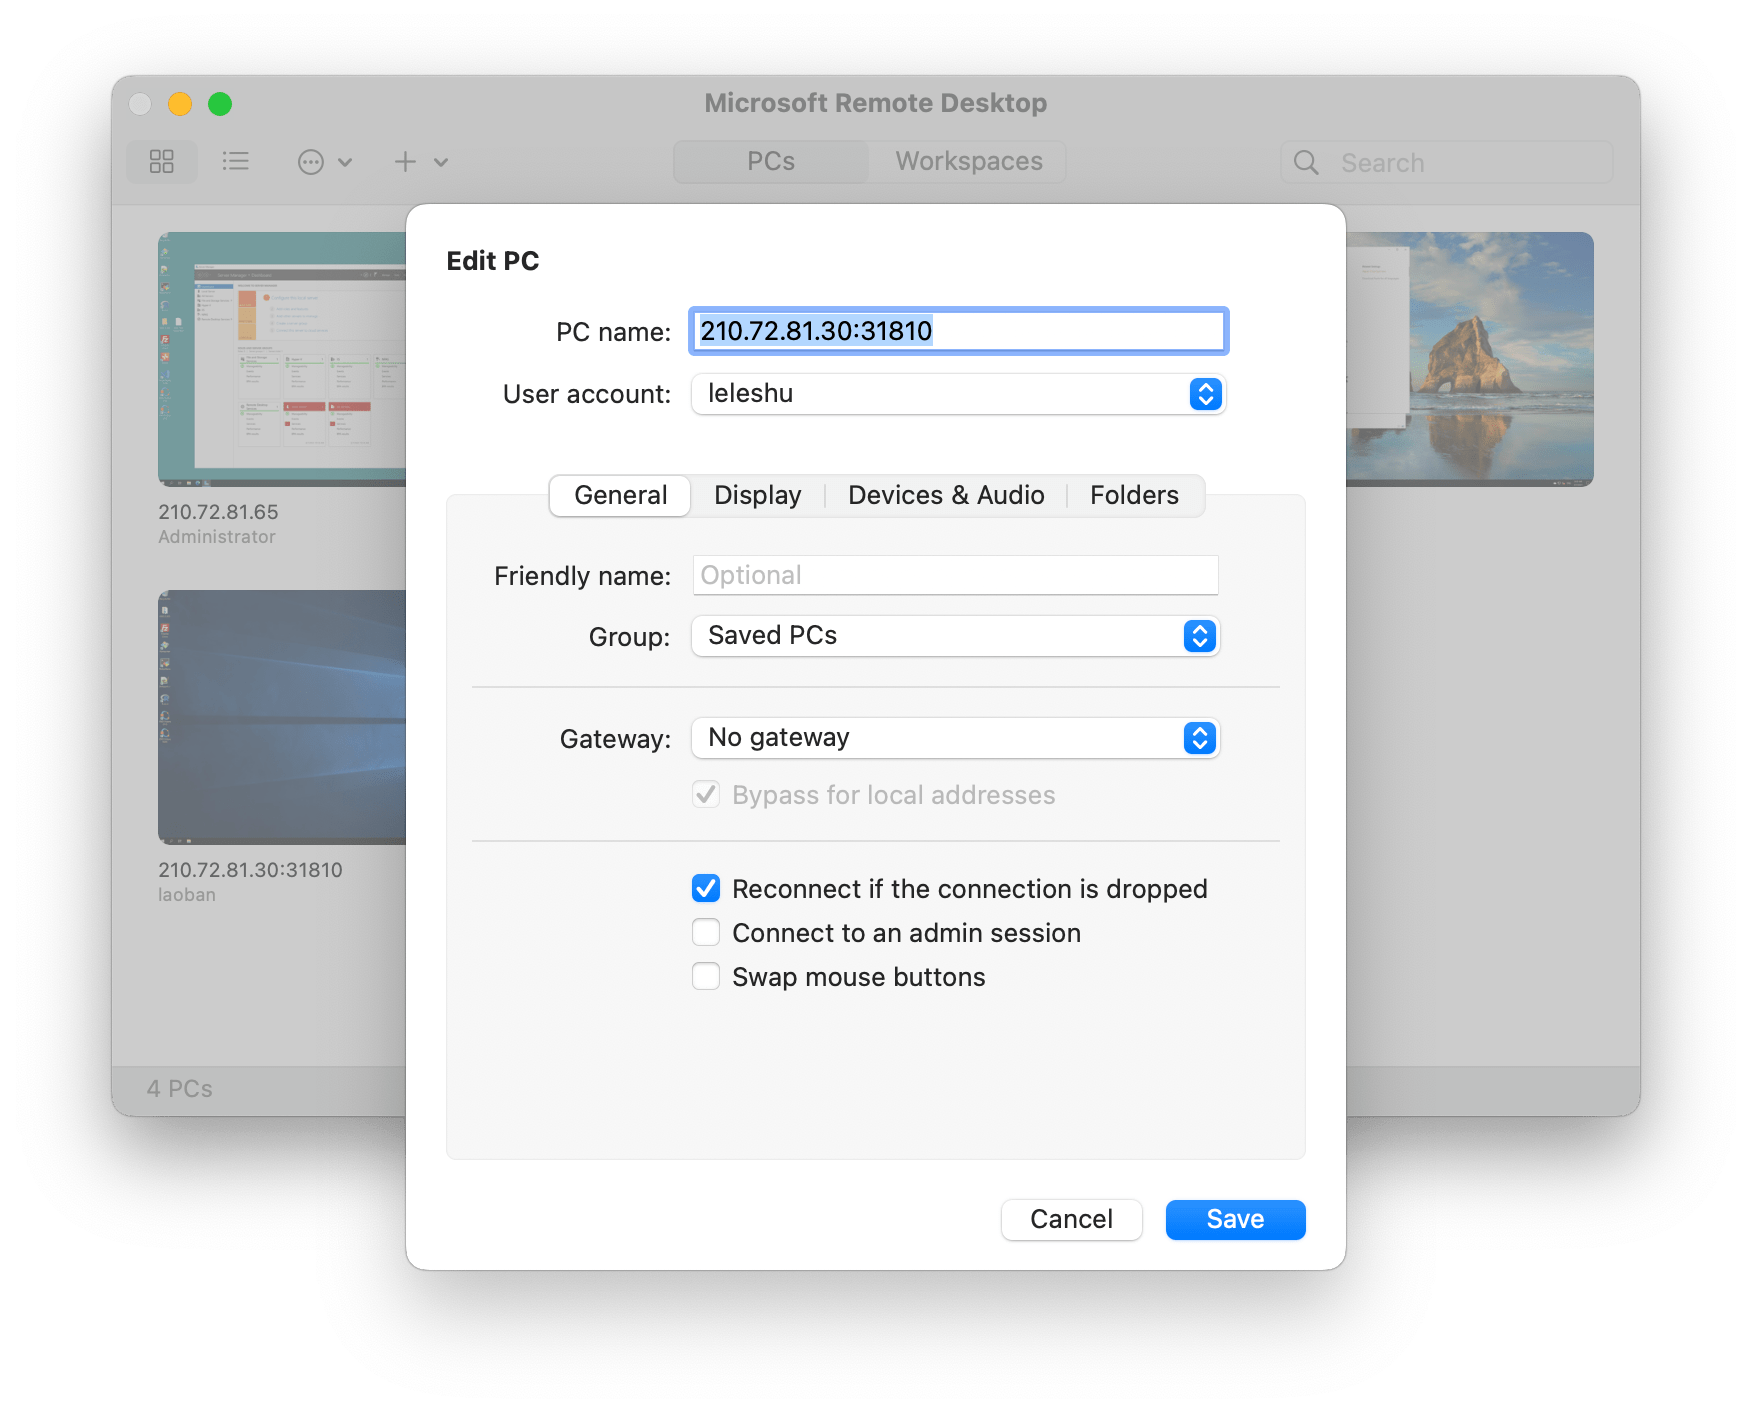
\includegraphics{Fig/ch5/rdp-2.png}
\caption{Microsoft Remote Desktop登录配置}
\end{figure}

\hypertarget{ubuntuux670dux52a1ux5668}{%
\section{Ubuntu服务器}\label{ubuntuux670dux52a1ux5668}}

服务器硬件配置

\begin{longtable}[]{@{}cccc@{}}
\toprule\noalign{}
类别 & 配件 & 参数 & 备注 \\
\midrule\noalign{}
\endhead
\bottomrule\noalign{}
\endlastfoot
平台 & 浪潮雷神SA5212 H5 & 12盘位2U机架式服务器 & \\
CPU & 至强Xeon 金牌 6133 & 每CPU 20核40线程,2.5GHz & 双CPU \\
内存 & 16GB x12 & DDR4 2666Mhz, 16 GBx12 & 6通道内存,12条 \\
硬盘 & U.2 NVME & 2TB & \\
网卡 & & 10Gbps 光口 & 两路光纤 \\
\end{longtable}

\hypertarget{ux64cdux4f5cux7cfbux7edfux4e0eux8f6fux4ef6-1}{%
\subsection{操作系统与软件}\label{ux64cdux4f5cux7cfbux7edfux4e0eux8f6fux4ef6-1}}

\begin{itemize}
\tightlist
\item
  操作系统:Ubuntu 20.04, 支持远程GUI登录。
\item
  远程桌面系统:xfce4
\item
  GIS软件:QGIS 3.10
\item
  R: R, Rstudio
\item
  Octave
\end{itemize}

\begin{figure}
\centering
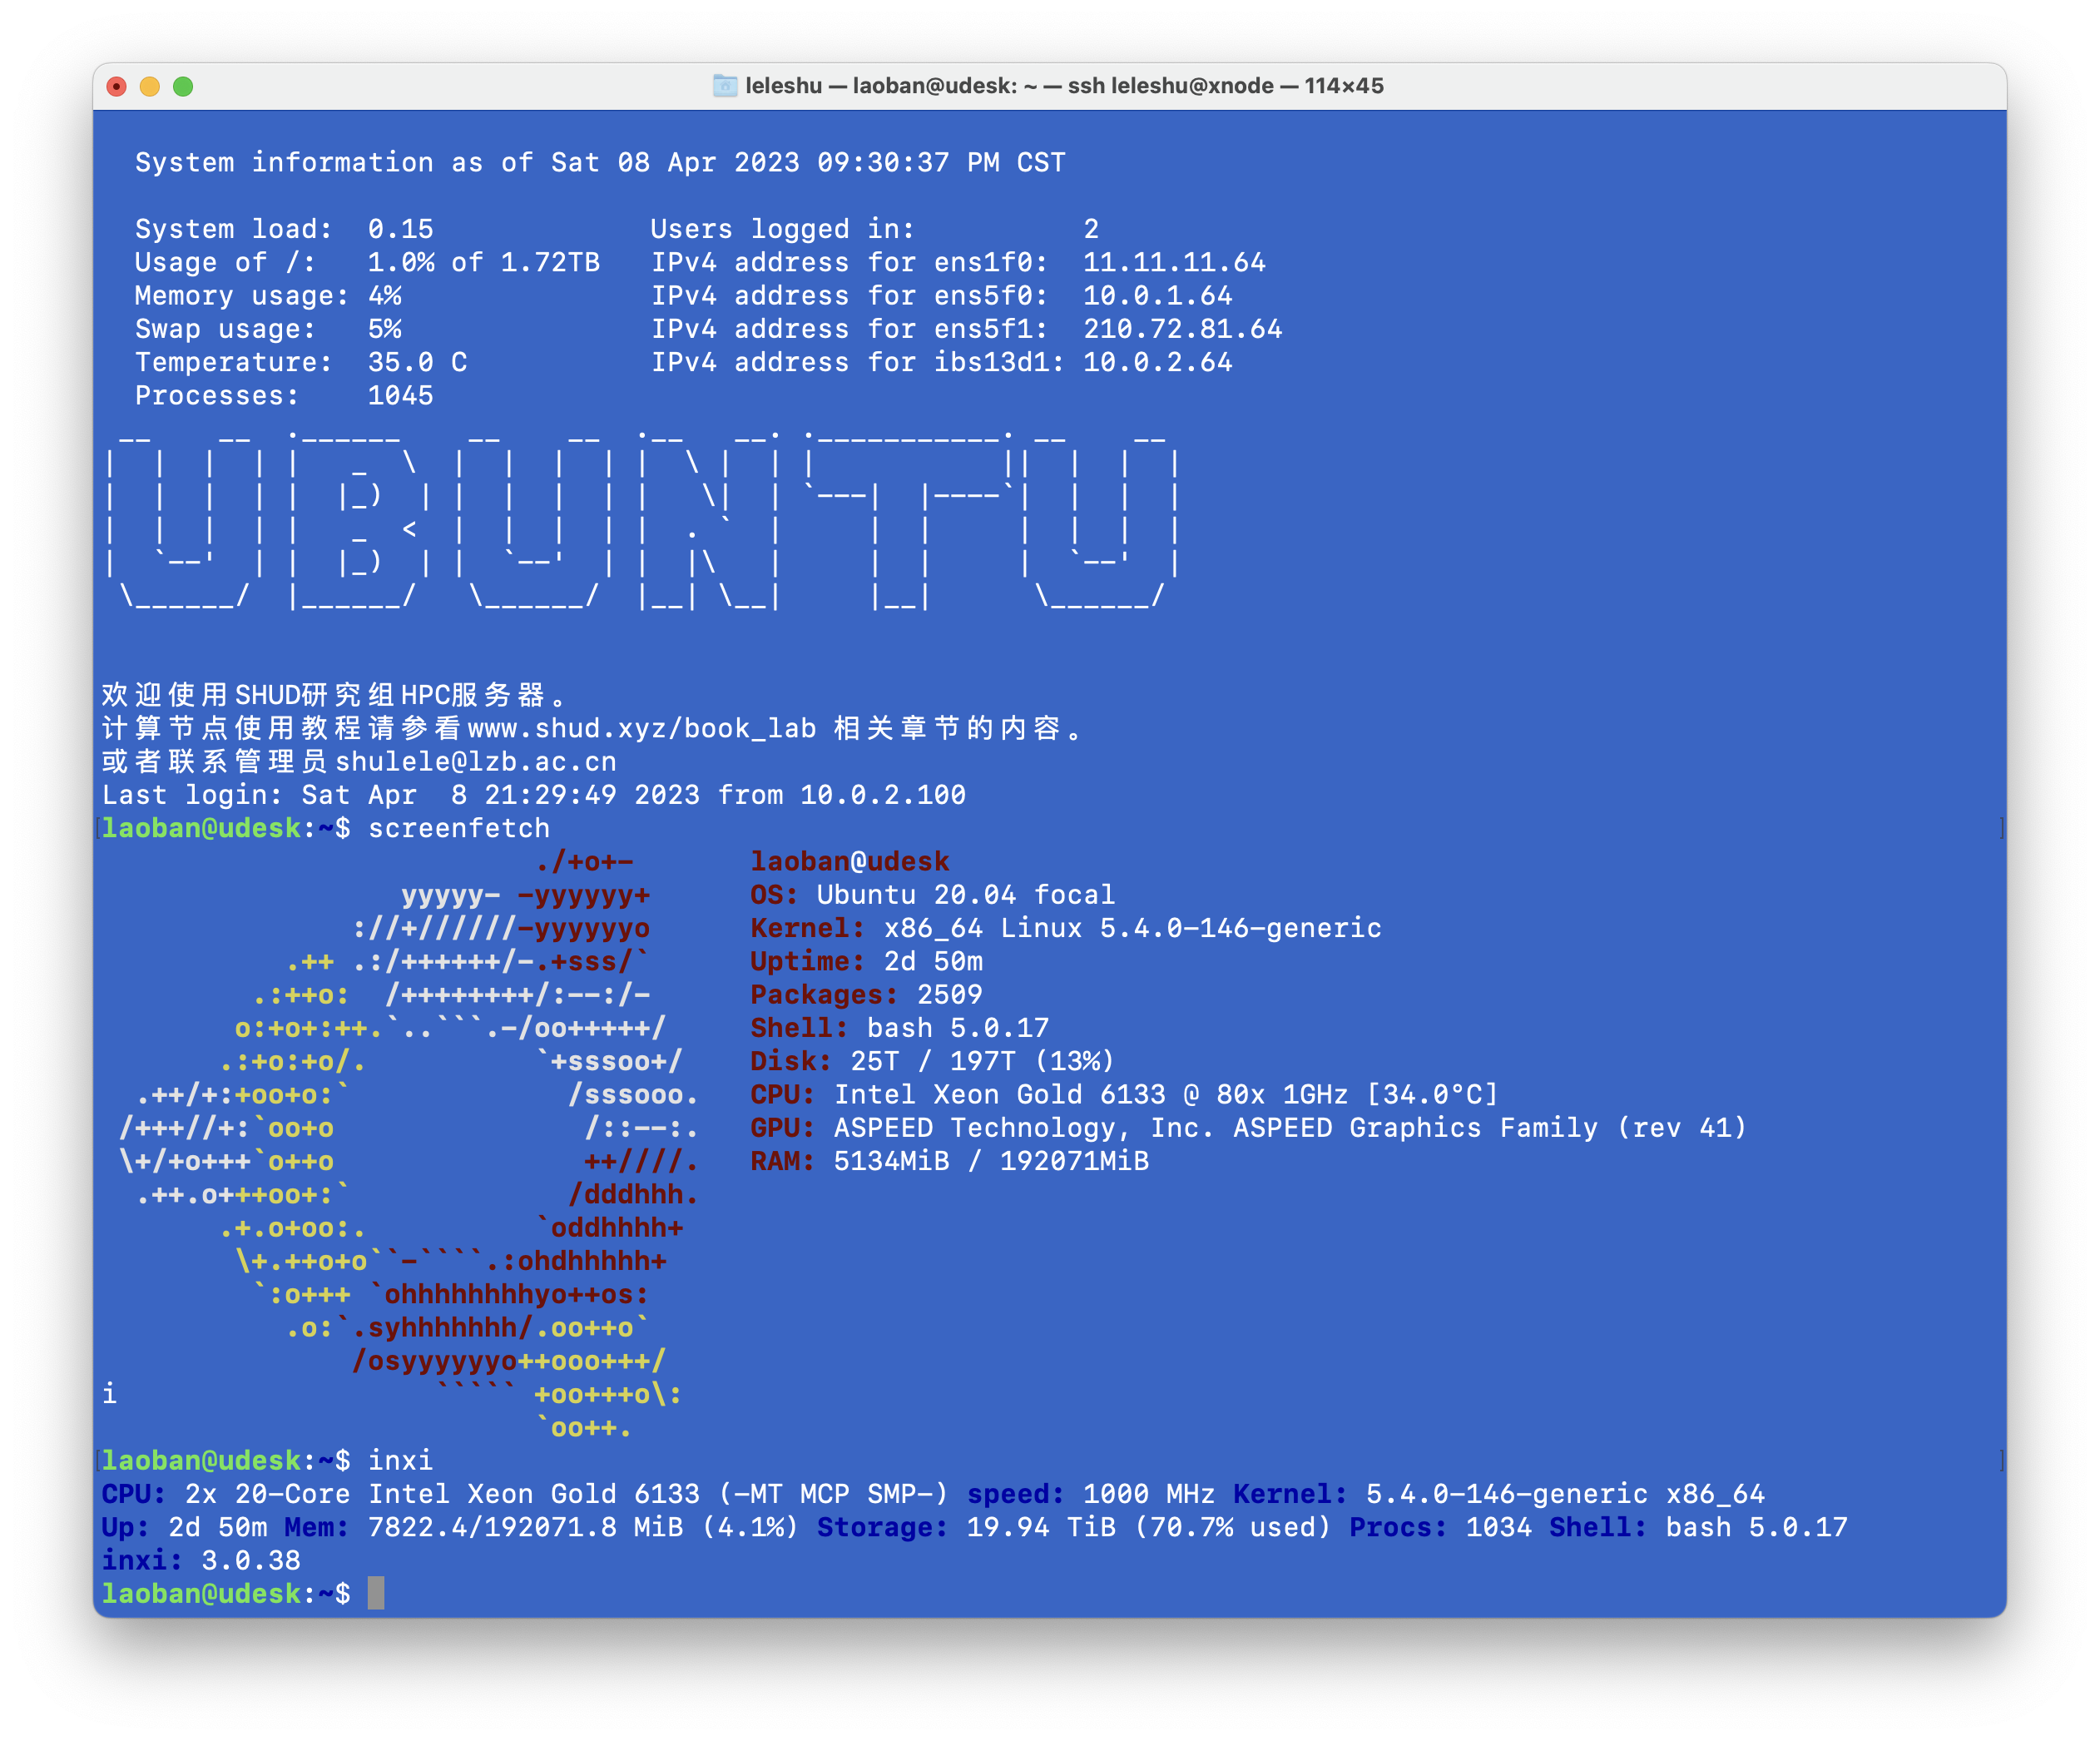
\includegraphics{Fig/ch5/host_udesk.png}
\caption{uDesk基本配置}
\end{figure}

\hypertarget{sshux767bux5f55}{%
\subsection{SSH登录}\label{sshux767bux5f55}}

\textbf{公网IP登录}

\begin{itemize}
\tightlist
\item
  登录IP: 210.77.77.23
\item
  软件:ssh (命令行);
\item
  端口: 32099
\end{itemize}

示例:

\begin{verbatim}
ssh zhangsan@210.77.77.23
\end{verbatim}

\textbf{路由器转发登录}

\begin{itemize}
\tightlist
\item
  登录IP: 210.77.77.25
\item
  软件:ssh;
\item
  端口: 32022
\end{itemize}

\begin{longtable}[]{@{}ll@{}}
\toprule\noalign{}
访问端口 & 服务器SSH端口 \\
\midrule\noalign{}
\endhead
\bottomrule\noalign{}
\endlastfoot
32022 & 32099 \\
\end{longtable}

示例:

\begin{verbatim}
ssh -p 32022 zhangsan@210.77.77.23
\end{verbatim}

\hypertarget{vncux8fdcux7a0bux684cux9762}{%
\subsection{VNC远程桌面}\label{vncux8fdcux7a0bux684cux9762}}

\begin{itemize}
\tightlist
\item
  软件:VNC (远程桌面)
\item
  端口: 共20个端口,最多支持20个VNC远程桌面,端口对应关系如下表:
\end{itemize}

\begin{longtable}[]{@{}cc@{}}
\toprule\noalign{}
访问端口 & 服务器VNC端口 \\
\midrule\noalign{}
\endhead
\bottomrule\noalign{}
\endlastfoot
32001 & 5901 \\
32002 & 5902 \\
32003 & 5903 \\
320xx & 59xx \\
32020 & 5920 \\
\end{longtable}

Ubuntu服务器端配置:建立vnc密码,并修改\textasciitilde/.vnc/xstartup文件。

\begin{verbatim}
vncpasswd
touch ~/.vnc/xstartup
chmod +x ~/.vnc/xstartup
vim ~/.vnc/xstartup
\end{verbatim}

在文件中输入文件内容:

\begin{verbatim}
#!/bin/sh
unset SESSION_MANAGER
unset DBUS_SESSION_BUS_ADDRESS
startxfce4 &
\end{verbatim}

登录远程桌面:
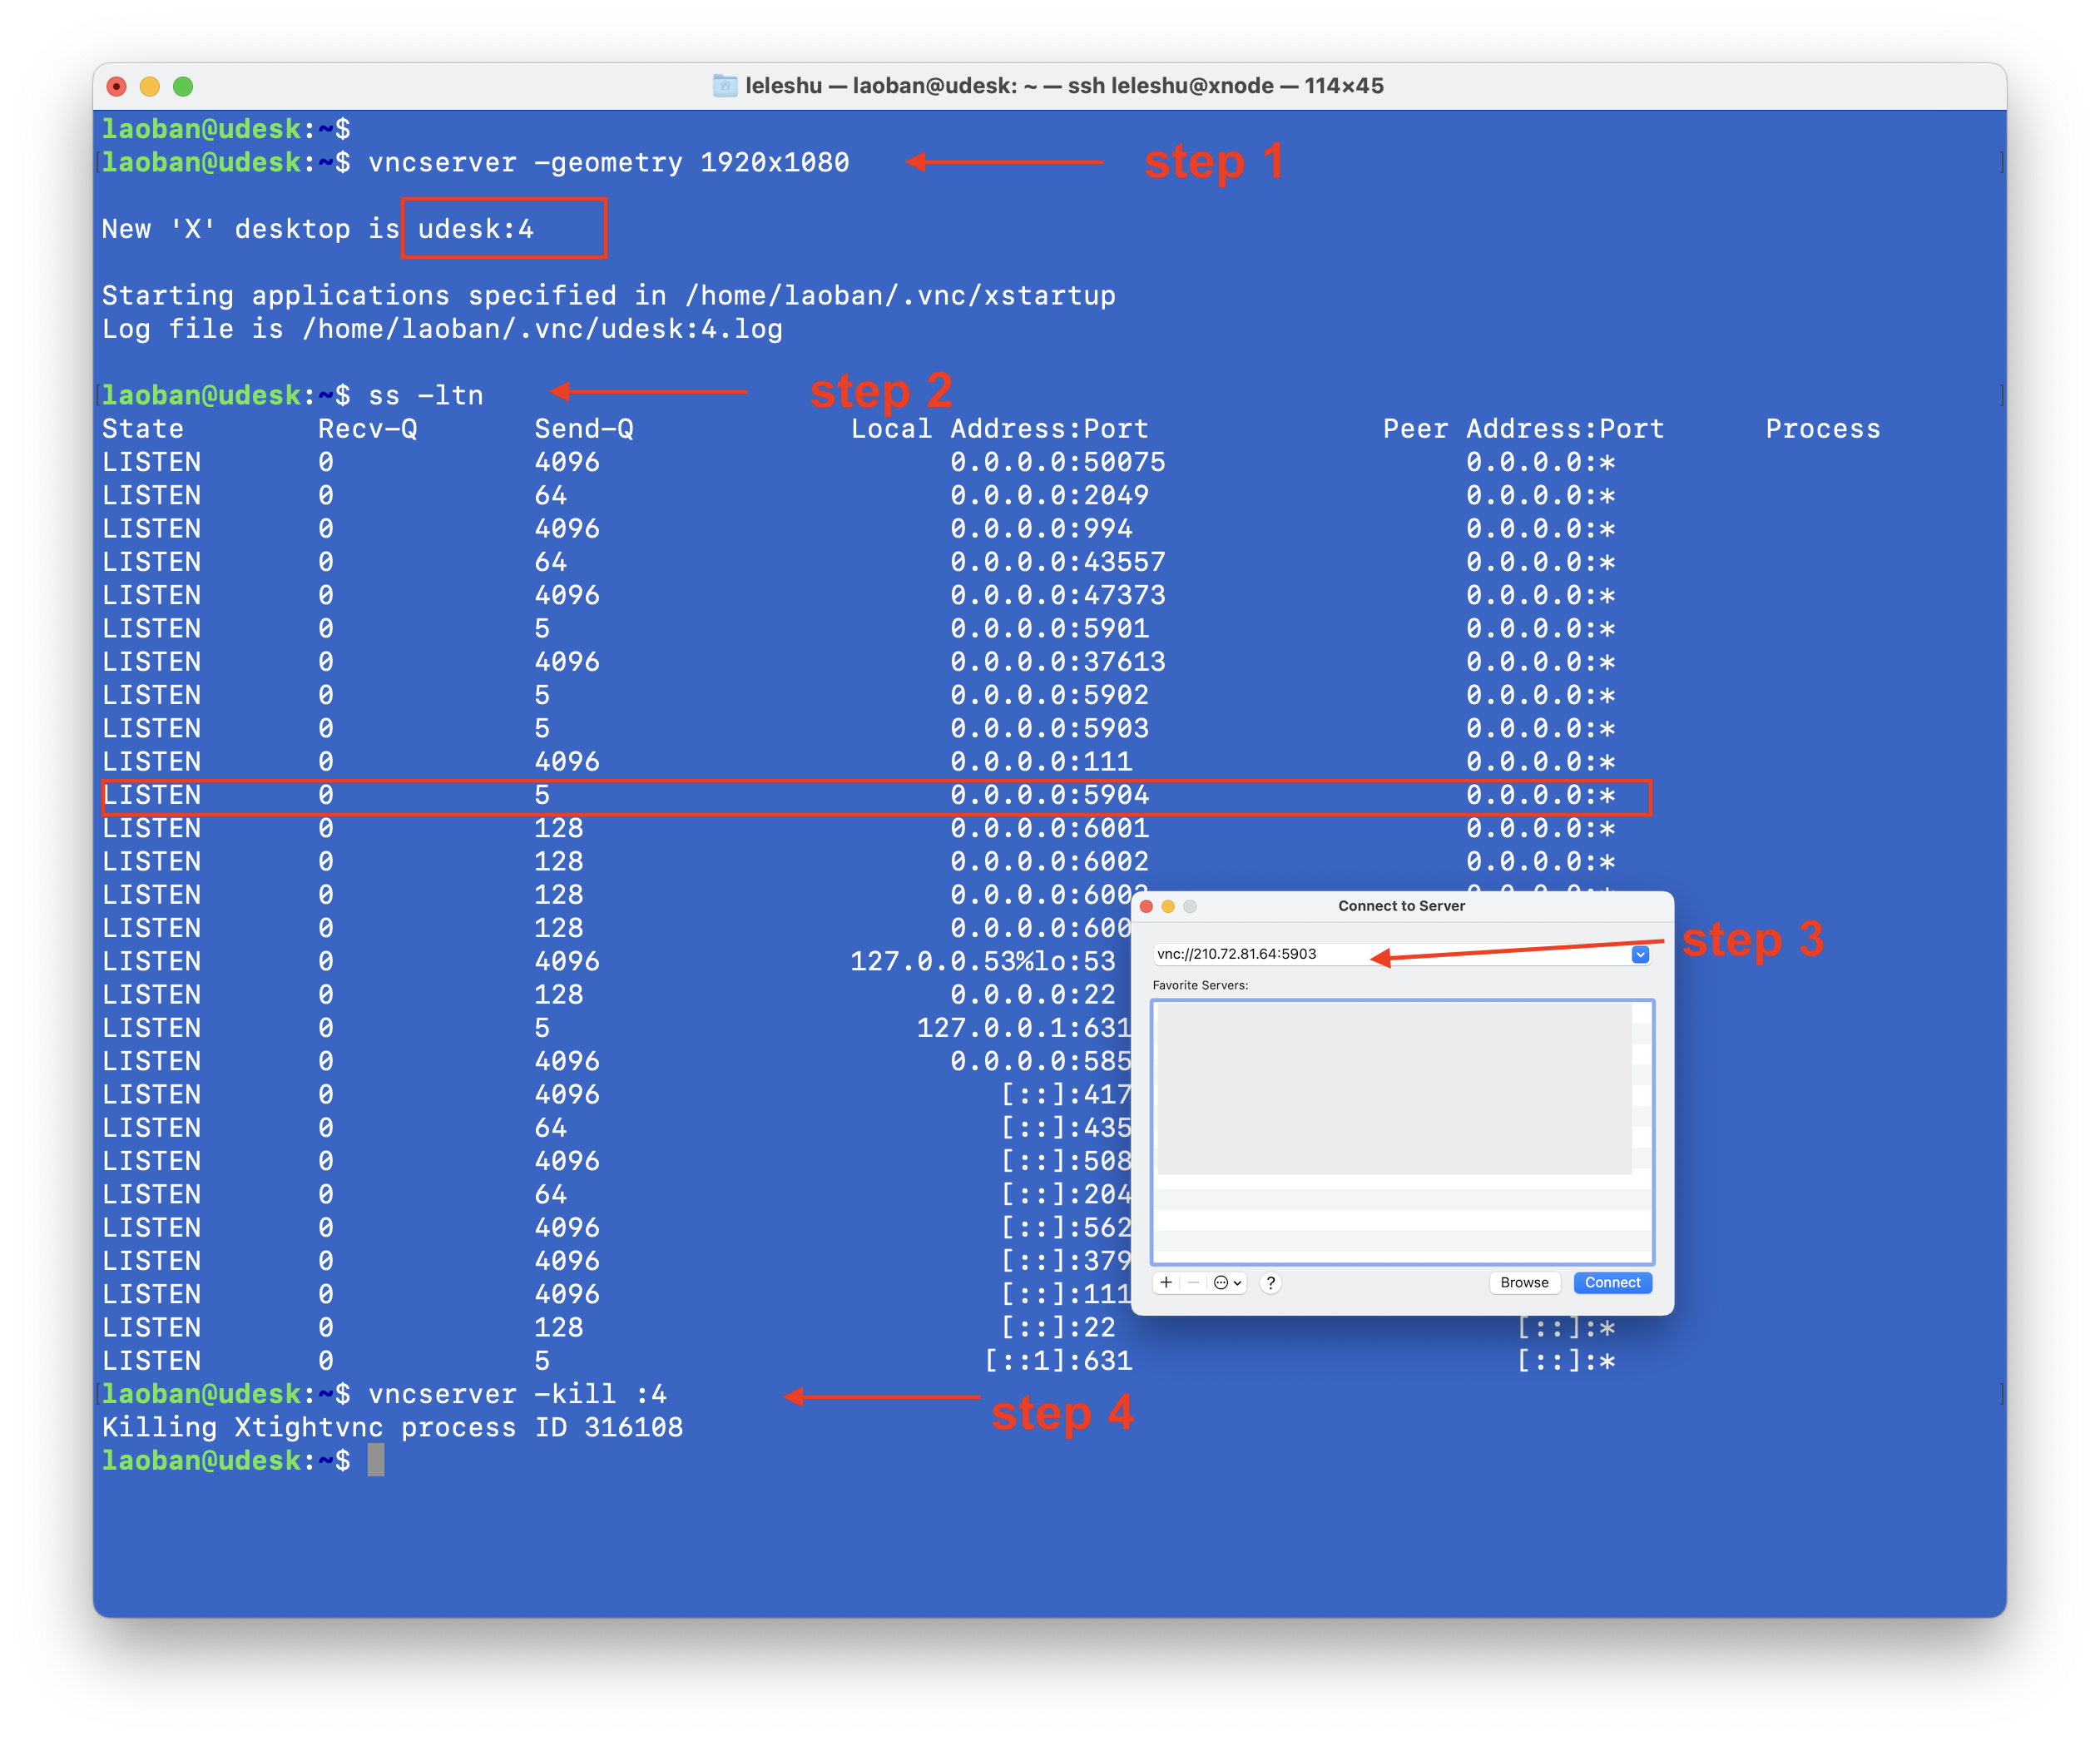
\includegraphics{Fig/ch5/udesk_RD.png}

\begin{enumerate}
\def\labelenumi{\arabic{enumi}.}
\item
  在服务器端启动vncserver。 \texttt{-geometry}参数可以设置远程桌面的分辨率。以下命令三选一

\begin{verbatim}
vncserver -geometry 1440x900
vncserver -geometry 1920x1080
vncserver -geometry 2560x1440
\end{verbatim}
\item
  然后使用\texttt{ss\ -ltn}当前vnc桌面的端口号码,默认第一个vnc桌面端口号为5901,第二个为5902,以此类推。或者通过命令\texttt{server\ -list}查看。 使用路由器端口转发,需要将590x的端口转换为320xx的端口,转换规则见前表。如果直接使用服务器公网IP,则直接使用590x端口。
\item
  在客户端启动vnc工具,访问{[}serverIP{]}:{[}端口号{]}。
  如使用公网IP,且vnc服务端口为5904:

\begin{verbatim}
vnc://210.77.77.23:5904 
\end{verbatim}

  如使用路由器IP,且vnc服务端口为5904,则转发端口为32004:

\begin{verbatim}
vnc://210.77.77.25:32004
\end{verbatim}
\item
  完成远程桌面工作后,退出vncserver时,需要关闭响应的vnc服务器,请在远程服务器端输入:

\begin{verbatim}
vncserver -kill :4
\end{verbatim}
\end{enumerate}

\textbf{使用完远程桌面,请主动关闭该vncserver}

\hypertarget{shudhpcux9ad8ux6027ux80fdux8ba1ux7b97ux96c6ux7fa4}{%
\section{SHUDHPC高性能计算集群}\label{shudhpcux9ad8ux6027ux80fdux8ba1ux7b97ux96c6ux7fa4}}

高性能计算机(High-performance computer,HPC)是由多台计算机构成的服务集群(cluster)。HPC主要由计算服务器、管理服务器和存储服务器组成,但只设有一个登录入口。用户登录到HPC后,只需将需要计算的相关任务提交至超算平台,平台计算任务调度系统将根据任务的需求和实际可用资源对任务进行排队和资源分配。

\begin{figure}
\centering
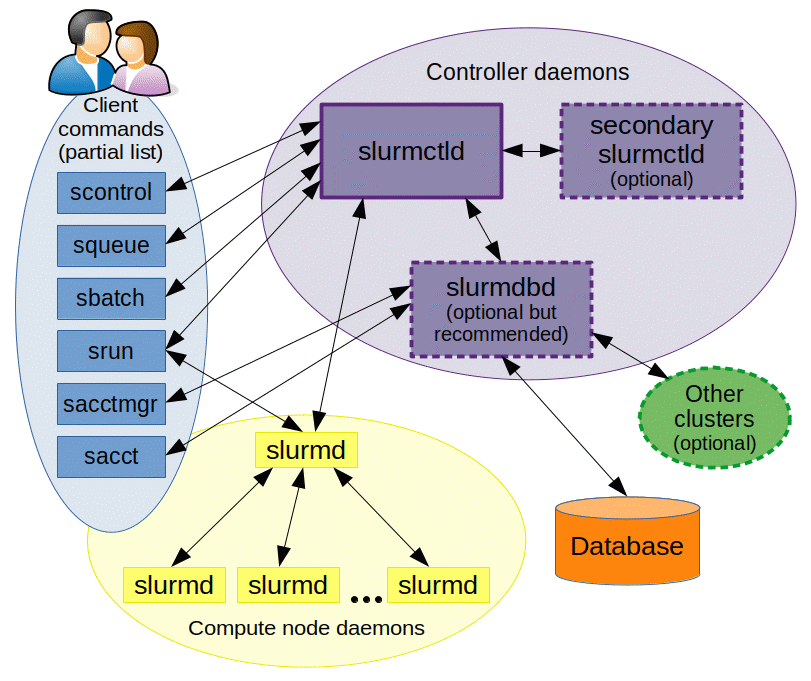
\includegraphics{Fig/ch5/slurm_arch.png}
\caption{slurm集群基本结构(来自:\url{https://slurm.schedmd.com/overview.html})}
\end{figure}

\hypertarget{ux767bux5f55}{%
\subsection{登录}\label{ux767bux5f55}}

\begin{itemize}
\tightlist
\item
  访问地址: \textbf{shud.vip}
\item
  ssh端口:32099
\item
  网页SSH访问:\textbf{ssh.shud.vip}
\item
  RStudio Server访问: \textbf{rstudio.shud.vip}
\end{itemize}

\hypertarget{ux670dux52a1ux5668ux786cux4ef6ux914dux7f6e}{%
\subsection{服务器硬件配置}\label{ux670dux52a1ux5668ux786cux4ef6ux914dux7f6e}}

\begin{longtable}[]{@{}
  >{\centering\arraybackslash}p{(\columnwidth - 6\tabcolsep) * \real{0.2414}}
  >{\centering\arraybackslash}p{(\columnwidth - 6\tabcolsep) * \real{0.2759}}
  >{\centering\arraybackslash}p{(\columnwidth - 6\tabcolsep) * \real{0.2414}}
  >{\centering\arraybackslash}p{(\columnwidth - 6\tabcolsep) * \real{0.2414}}@{}}
\toprule\noalign{}
\begin{minipage}[b]{\linewidth}\centering
大类
\end{minipage} & \begin{minipage}[b]{\linewidth}\centering
平台
\end{minipage} & \begin{minipage}[b]{\linewidth}\centering
参数
\end{minipage} & \begin{minipage}[b]{\linewidth}\centering
备注
\end{minipage} \\
\midrule\noalign{}
\endhead
\bottomrule\noalign{}
\endlastfoot
平台 & 高性能计算集群 & 8计算节点,1登录节点,1高速存储 & 56G IB网络, 10G 以太网 \\
登录节点 & 超聚变2288 V6 & 2x 至强6318Y (56核),128G,2TB U.2 NVME & \\
存储 & 超聚变2288 V6 & 14x 16TB, RAID 5 & 173TB可用 \\
全闪存储 & 泰安3036 & 12x 3.76TB, ZFS RAIDZ2 & 34TB可用 \\
计算节点 & 超微八节点高密计算平台 & 每节点:至强6133 40核(2x 20),192GB内存 & \\
IB交换机 & SX6025 & 36x 56Gbps & InfiniBand \\
万兆以太交换机 & IBM & 48x 10Gbps,4x 40Gbps & 全光口 \\
千兆以太交换机 & H3C & 48x 1Gbps & 全光口 \\
\end{longtable}

\hypertarget{shudhpc-ipux5730ux5740ux914dux7f6e}{%
\subsection{SHUDHPC IP地址配置}\label{shudhpc-ipux5730ux5740ux914dux7f6e}}

\begin{longtable}[]{@{}cccc@{}}
\toprule\noalign{}
节点 & 主机名 & 万兆IP & InfiniBand IP地址 \\
\midrule\noalign{}
\endhead
\bottomrule\noalign{}
\endlastfoot
登录节点 & xnode & 10.0.1.100 & 10.0.2.100 \\
全闪存储 & flash & 10.0.1.99 & 10.0.2.99 \\
存储 & stor & 10.0.1.100 & 10.0.2.100 \\
计算节点 & cn{[}01-08{]} & 10.0.1.101\textasciitilde108 & 10.0.2.101\textasciitilde108 \\
\end{longtable}

\hypertarget{ux64cdux4f5cux7cfbux7edfux4e0eux8f6fux4ef6-2}{%
\subsection{操作系统与软件}\label{ux64cdux4f5cux7cfbux7edfux4e0eux8f6fux4ef6-2}}

\begin{itemize}
\tightlist
\item
  操作系统:Ubuntu 20.04, 仅支持命令行登录。
\item
  作业调度:slurm
\item
  R: R
\item
  Octave
\end{itemize}

\hypertarget{ux5b58ux50a8ux4fe1ux606f}{%
\subsection{存储信息}\label{ux5b58ux50a8ux4fe1ux606f}}

假设用户名为\textbf{zhangsan}

\begin{longtable}[]{@{}
  >{\centering\arraybackslash}p{(\columnwidth - 6\tabcolsep) * \real{0.1515}}
  >{\centering\arraybackslash}p{(\columnwidth - 6\tabcolsep) * \real{0.1515}}
  >{\centering\arraybackslash}p{(\columnwidth - 6\tabcolsep) * \real{0.1515}}
  >{\raggedright\arraybackslash}p{(\columnwidth - 6\tabcolsep) * \real{0.5455}}@{}}
\toprule\noalign{}
\begin{minipage}[b]{\linewidth}\centering
目录
\end{minipage} & \begin{minipage}[b]{\linewidth}\centering
所属
\end{minipage} & \begin{minipage}[b]{\linewidth}\centering
权限
\end{minipage} & \begin{minipage}[b]{\linewidth}\raggedright
使用规则
\end{minipage} \\
\midrule\noalign{}
\endhead
\bottomrule\noalign{}
\endlastfoot
/volume/repo/zhangsan & 用户冷数据空间 & 700 & 用于存放用户程序、文件等,限10TB容量 \\
/users/zhangsan & 用户主目录 & 700 & 仅用于编译、文件库等文件存放;禁止大文件,禁止计算。 \\
/scratch/zhangsan & 高速计算空间 & 700 & 可进行计算任务,任何超过60天的文件会自动删除 \\
/volume/data & 冷数据盘 & 777 & 公共空间。不要长期存储个人数据 \\
/tmp* & 临时数据 & 777 & 公共临时目录;如需高速运算,输出数据可存在/tmp里面 \\
/opt & 软件安装/编译盘 & 755 & 公共程序安装目录 \\
\end{longtable}

\textbf{注}:每一个计算节点上面都有/tmp目录,这个磁盘属于计算节点的U.2 NVME高速磁盘,写入速度约2000MB/s,计算结果存储在/tmp速度最快。但是,当计算完成后,用户无法访问计算节点的/tmp。例如:用户在主节点xnode上提交任务(./shud -o /tmp/ccw.out ccw)给cn01节点,计算过程中,cn01上的任务将结果保存在cn01:/tmp/ccw.out里面。但是,当任务完成后,用户无法直接访问cn01:/tmp下的文件,用户只能访问到xnode:/tmp下的文件。 因此,如果任务提交时选择/tmp写出,那么需要在任务脚本中加入一个拷贝/tmp/ccw.out到用户个人目录的命令,以此保证用户可以获得计算结果。

\hypertarget{ux7528ux6237ux7ba1ux7406}{%
\subsection{用户管理}\label{ux7528ux6237ux7ba1ux7406}}

\begin{itemize}
\tightlist
\item
  zhangsan: 一般用户
\end{itemize}

研究组的每个成员将获得一个登录账号,账号类型为超算一般用户,具有提交任务的权限。如果任务需要特殊要求,请与PI进行沟通。

\hypertarget{ux4f5cux4e1aux7ba1ux7406slurm}{%
\subsection{作业管理Slurm}\label{ux4f5cux4e1aux7ba1ux7406slurm}}

SLURM (Simple Linux Utility for Resource Management) 是一个流行的开源的作业调度和集群管理系统,主要用于高性能计算和科学计算领域。SLURM的主要特点包括:灵活的资源管理、可扩展性、高可用性、高可靠性、多种作业调度算法和管理工具等。

在SLURM中,用户提交的作业会被分配到可用的计算节点上进行计算。SLURM会根据可用资源的情况,按照用户指定的优先级和作业调度算法来安排作业的执行顺序,以达到最大化集群的利用率和性能。同时,SLURM还提供了一系列管理工具,如节点管理、队列管理、用户管理、资源限制等,方便管理员对集群进行管理和监控。

SLURM的使用十分广泛,被许多知名的超算中心采用。

当前八个计算节点全部归属同一个计算分区(partition)。\texttt{partition\ =\ suan}。

命令代码

\begin{verbatim}
srun -N 5 -n 5 hostname  #5个节点,5个CPU
srun -N 5 -n 50 hostname  #5个节点,50个CPU
\end{verbatim}

代码示例1:

\begin{verbatim}
#!/bin/bash
#SBATCH --job-name=hostname
#SBATCH --partition=suan # 计算分区名称。
#SBATCH -N 1 # 计算节点数量
#SBATCH --mail-type=end  
#SBATCH --mail-user=YOU@EMAIL.COM
#SBATCH --output=%j.out  # 屏幕输出文件
#SBATCH --error=%j.err  # 屏幕错误信息输出文件。

/bin/hostname
\end{verbatim}

以上代码保存为\texttt{submit1.sh}。 然后在命令行中执行以下命令:

\begin{verbatim}
sbatch submit1.sh
\end{verbatim}

代码示例2:

\begin{verbatim}
#!/bin/bash
#
#SBATCH --job-name=echo_number # 任务名称
#SBATCH --output=slurm_%j.out # 屏幕输出及错误信息输出文件。
#SBATCH --ntasks=30  # CPU数量。

for i in {2000..2030}
do
    srun -n1  --exact  echo  $i &
done
wait
\end{verbatim}

开启交互模式

\begin{verbatim}
srun --nodes=1 --ntasks-per-node=1 --time=01:00:00 --pty bash -i
\end{verbatim}

\textbf{最简单的SHUD模型slurm任务案例:}
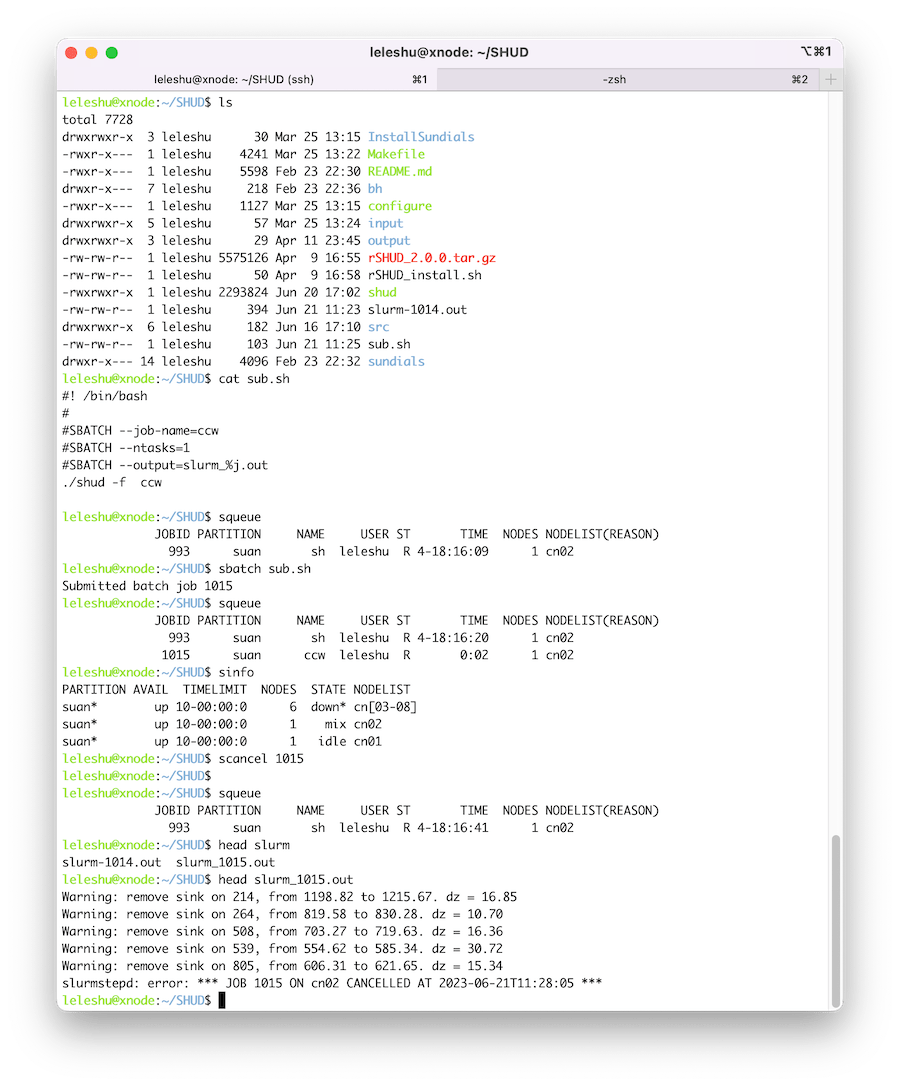
\includegraphics{Fig/ch5/slurm_example.png}

slurm教程参考

\begin{itemize}
\tightlist
\item
  上海交大: \url{https://docs.hpc.sjtu.edu.cn/job/slurm.html}
\item
  北京大学:\url{https://hpc.pku.edu.cn/_book/}
\end{itemize}

\hypertarget{slurmux4f7fux7528ux6ce8ux610fux4e8bux9879}{%
\subsection{Slurm使用注意事项}\label{slurmux4f7fux7528ux6ce8ux610fux4e8bux9879}}

\begin{enumerate}
\def\labelenumi{\arabic{enumi}.}
\tightlist
\item
  不要使用主节点进行计算工作,任务全部通过slurm提交到计算节点。
\item
  不要使用\texttt{exclusive}选项。如果确实有必要,请提前告知PI和其他组员。
\item
  如果计算任务的数据写入量巨大,临时数据(药渣数据)请存放到/tmp目录下------该文件夹是数据计算节点的/tmp;然后修改程序,在程序结束之后从/tmp目录下移动/复制数据到\texttt{/user/zhangsan},\texttt{/volume/repo/zhangsan}个人文件夹,再做数据后处理。
\end{enumerate}

注意,移动\texttt{/tmp}下文件的操作,比如在提交slurm的脚本或者程序中体现------因为,如果slurm计算任务结束之后,在主节点上访问的/tmp是主节点/tmp,无法再访问计算节点的/tmp文件夹。

\hypertarget{ResNormal}{%
\chapter{研究的范式}\label{ResNormal}}

\hypertarget{ux79d1ux5b66ux95eeux9898}{%
\section{科学问题}\label{ux79d1ux5b66ux95eeux9898}}

具体什么是科学问题,难有准确定义,但是我们可以从一些侧面了解什么是科学问题。

科学问题的一些诠释:

\begin{itemize}
\tightlist
\item
  一个你能通过科学实验方能解决的问题;
\item
  一个讨论过、研究过,但尚未形成定论的问题;
\item
  一个可能被你的科学设计而解决的问题。
\end{itemize}

\hypertarget{ux79d1ux5b66ux95eeux9898ux7684ux6848ux4f8b}{%
\subsection{科学问题的案例}\label{ux79d1ux5b66ux95eeux9898ux7684ux6848ux4f8b}}

\begin{longtable}[]{@{}cc@{}}
\toprule\noalign{}
案例 & 详细解释 \\
\midrule\noalign{}
\endhead
\bottomrule\noalign{}
\endlastfoot
& \\
\end{longtable}

\begin{quote}
\url{https://www.scribbr.com/research-process/research-question-examples/}
\end{quote}

\hypertarget{ux7814ux7a76ux533a}{%
\section{研究区}\label{ux7814ux7a76ux533a}}

\hypertarget{ux8d44ux6599ux6536ux96c6ux548cux5904ux7406}{%
\subsection{资料收集和处理}\label{ux8d44ux6599ux6536ux96c6ux548cux5904ux7406}}

\hypertarget{ux57faux672cux8d44ux6599}{%
\subsubsection{基本资料}\label{ux57faux672cux8d44ux6599}}

\begin{itemize}
\tightlist
\item
  社会经济发展:GDP,主要经济支柱
\item
  人口:人口分布以及人口时间变化,重要时间节点
\item
  行政归属
\end{itemize}

\hypertarget{ux5730ux7406ux6570ux636e}{%
\subsubsection{地理数据:}\label{ux5730ux7406ux6570ux636e}}

\begin{itemize}
\tightlist
\item
  高程:DEM,地形图
\item
  土地利用:不同分类体系下的土地利用;不同时期的土地利用
\item
  土壤质地:沙粉黏比例,土壤容重、有机质含量、土壤层厚度
\item
  地质背景
\item
  降雨分布
\item
  温度分布
\item
  行政边界:各级行政区划
\item
  城市/居民点
\item
  道路:各级公路铁路
\end{itemize}

\textbf{以上数据应当形成标准图件。}

\hypertarget{ux6c14ux8c61ux518dux5206ux6790ux8d44ux6599}{%
\subsubsection{气象再分析资料}\label{ux6c14ux8c61ux518dux5206ux6790ux8d44ux6599}}

\begin{itemize}
\tightlist
\item
  GLDAS
\item
  CMFD
\item
  PRISM
\end{itemize}

\hypertarget{skill}{%
\chapter{工作技能}\label{skill}}

\hypertarget{researchtool}{%
\section{科研工具}\label{researchtool}}

推荐使用的科研软件请先查看下面这张图。绝大部分为免费软件,个别是收费软件。
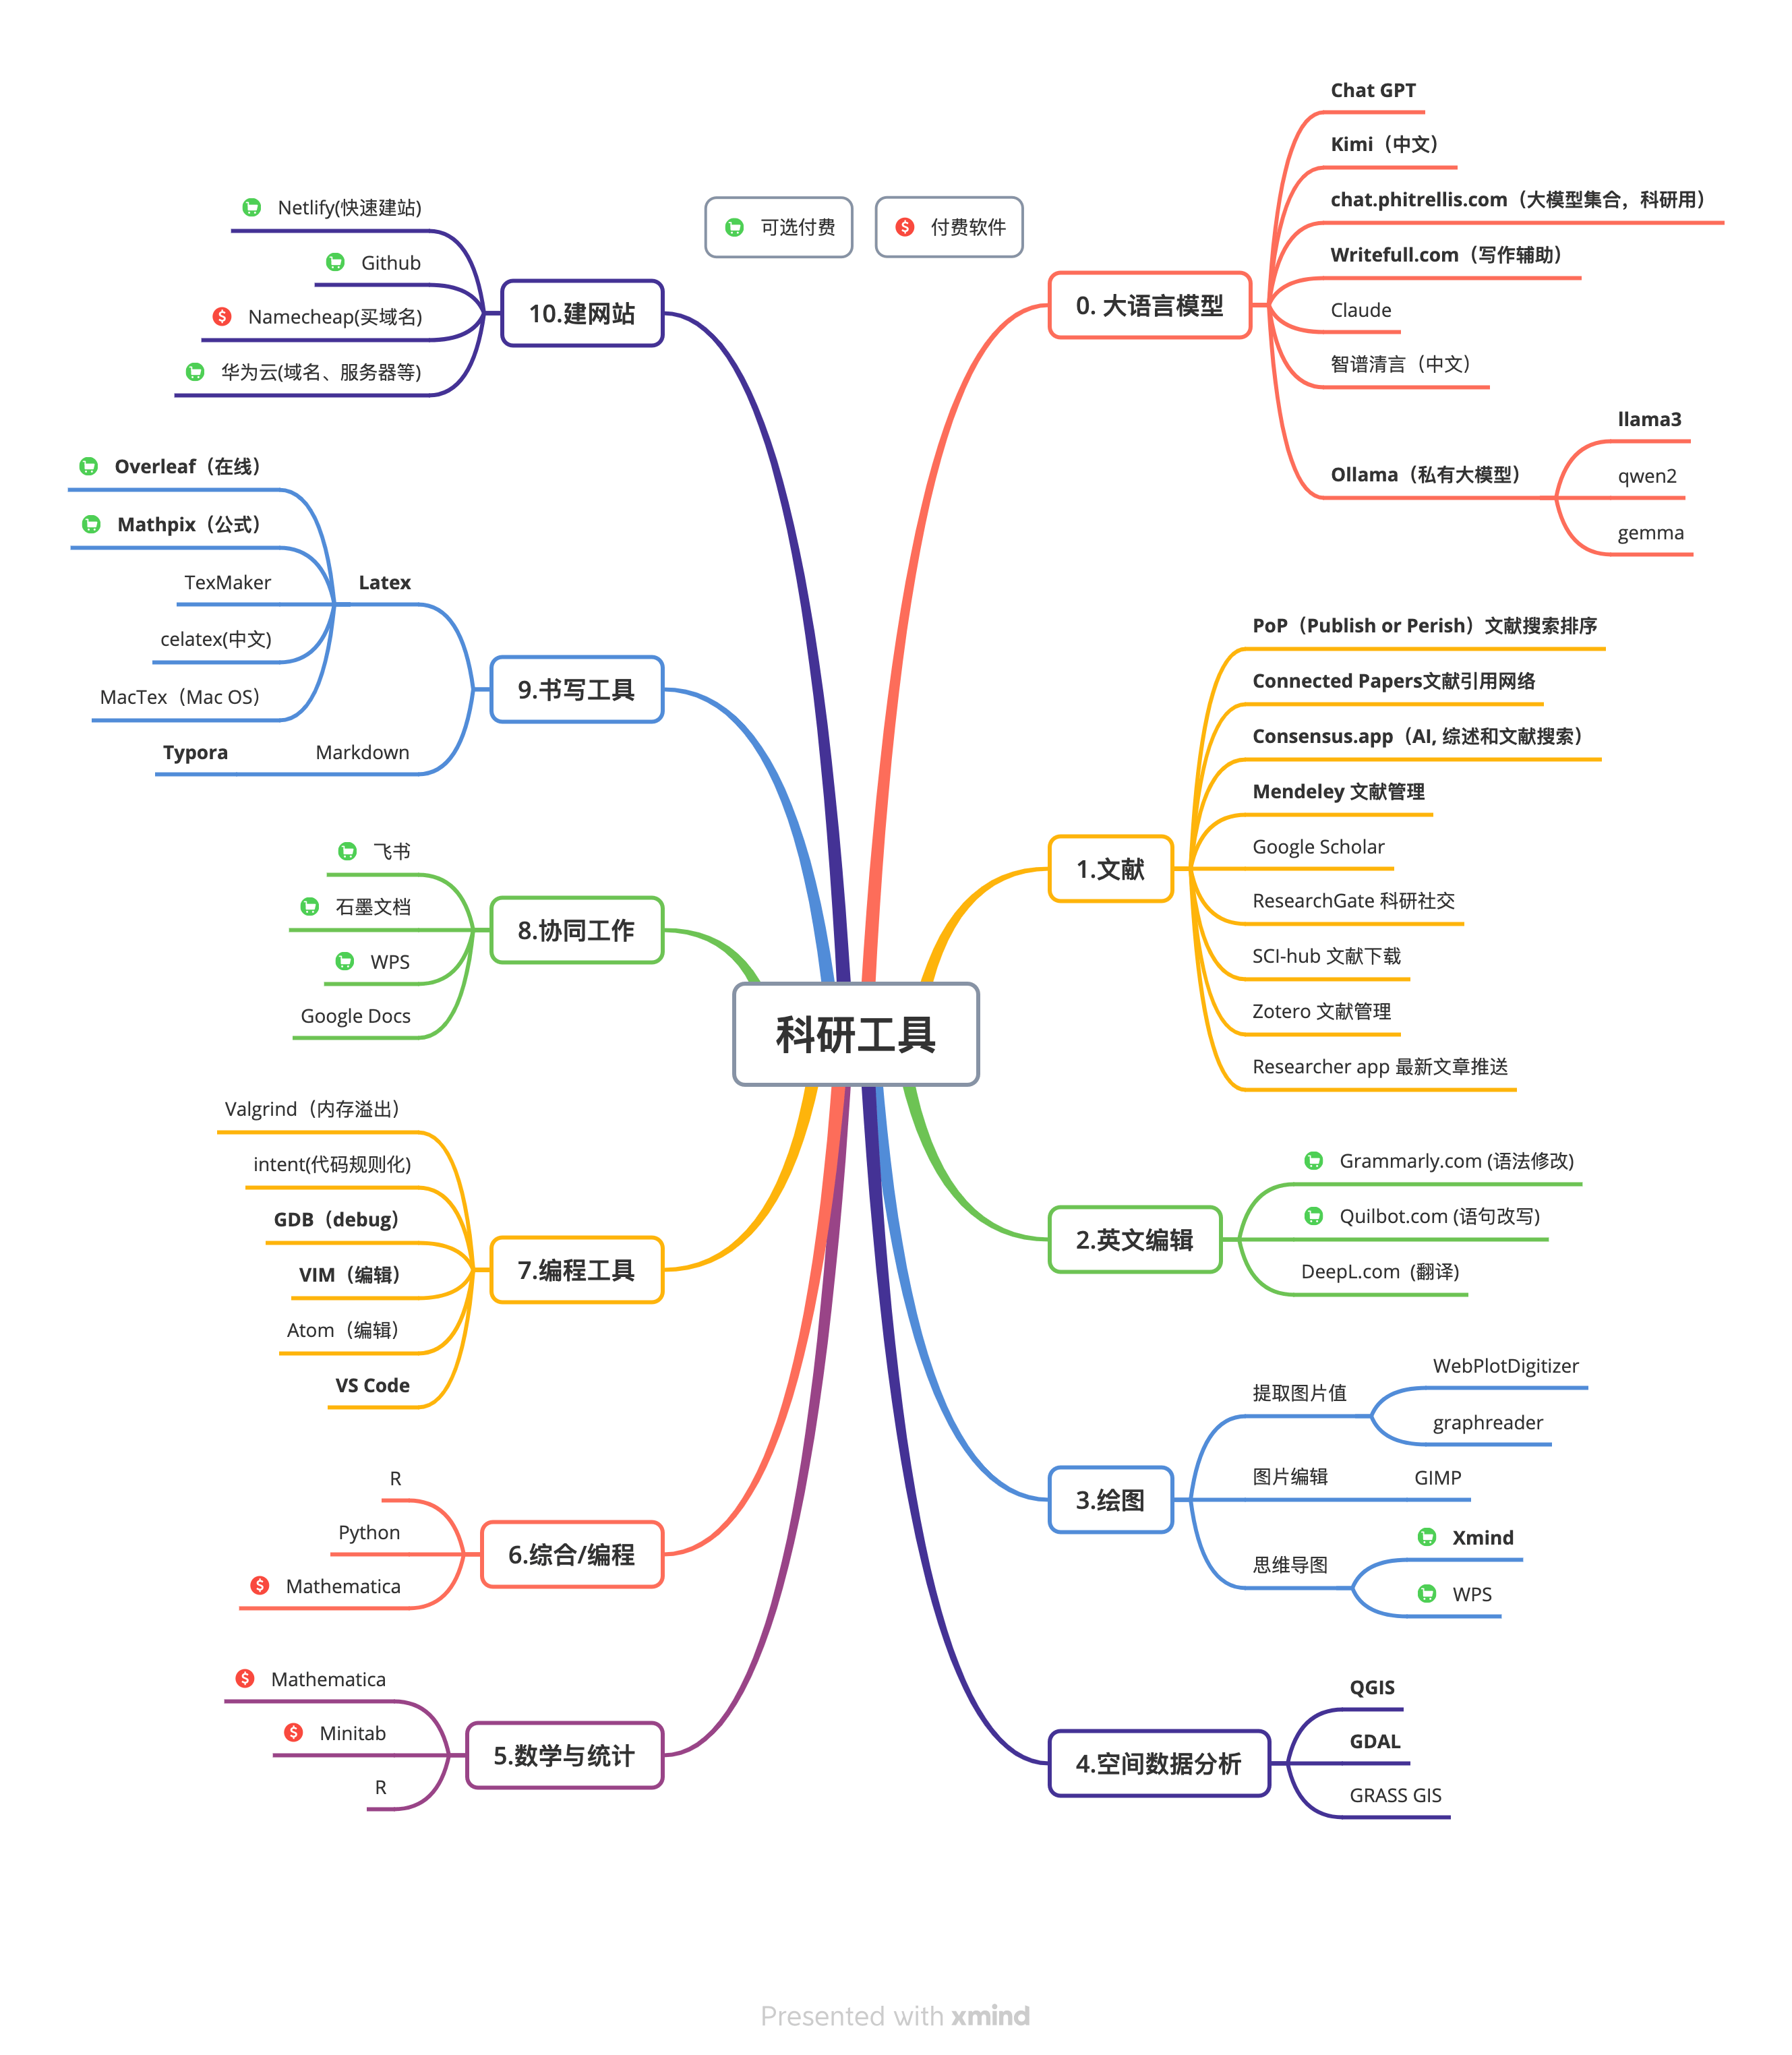
\includegraphics{Fig/tools.png}

\hypertarget{ux7a7aux95f4ux5236ux56feqgis}{%
\subsection{【空间制图】QGIS}\label{ux7a7aux95f4ux5236ux56feqgis}}

QGIS是一款免费、开源的地理信息系统(GIS)软件,相对于其他商业GIS软件,它有以下几个优势:

\begin{itemize}
\tightlist
\item
  \textbf{免费}:QGIS是一款完全免费的GIS软件,用户可以自由地下载、使用和修改它。
\item
  开源:QGIS是一个开源软件,这意味着用户可以随意查看其源代码、修改和扩展其功能,同时也可以通过用户社区获得技术支持。
\item
  \textbf{跨平台}:QGIS可以在Windows、MacOS、Linux等多个操作系统上运行,并提供相应的安装程序和二进制文件。
\item
  多功能:QGIS具有很多功能,包括地图制作、数据处理、空间分析、地理编码和地理数据编辑等。它支持许多不同的文件格式,包括ESRI shapefile、MapInfo文件、PostGIS和Oracle空间数据库、GeoTIFF和其他栅格数据格式等。
\item
  \textbf{易于使用}:QGIS提供了易于使用的用户界面,包括地图绘制、数据导入和空间分析等功能。此外,用户可以通过插件来扩展软件的功能,满足不同的需求。
\item
  社区支持:QGIS有一个活跃的用户社区,用户可以通过该社区获得技术支持、交流使用经验和分享资源等。
\end{itemize}

综上所述,QGIS是一款免费、开源、跨平台、功能丰富、易于使用且有着强大的社区支持的GIS软件。它是许多研究人员、学生和行业专业人士的首选工具之一。

下载地址:\url{https://www.qgis.org/en/site/forusers/download.html}

\begin{figure}
\centering
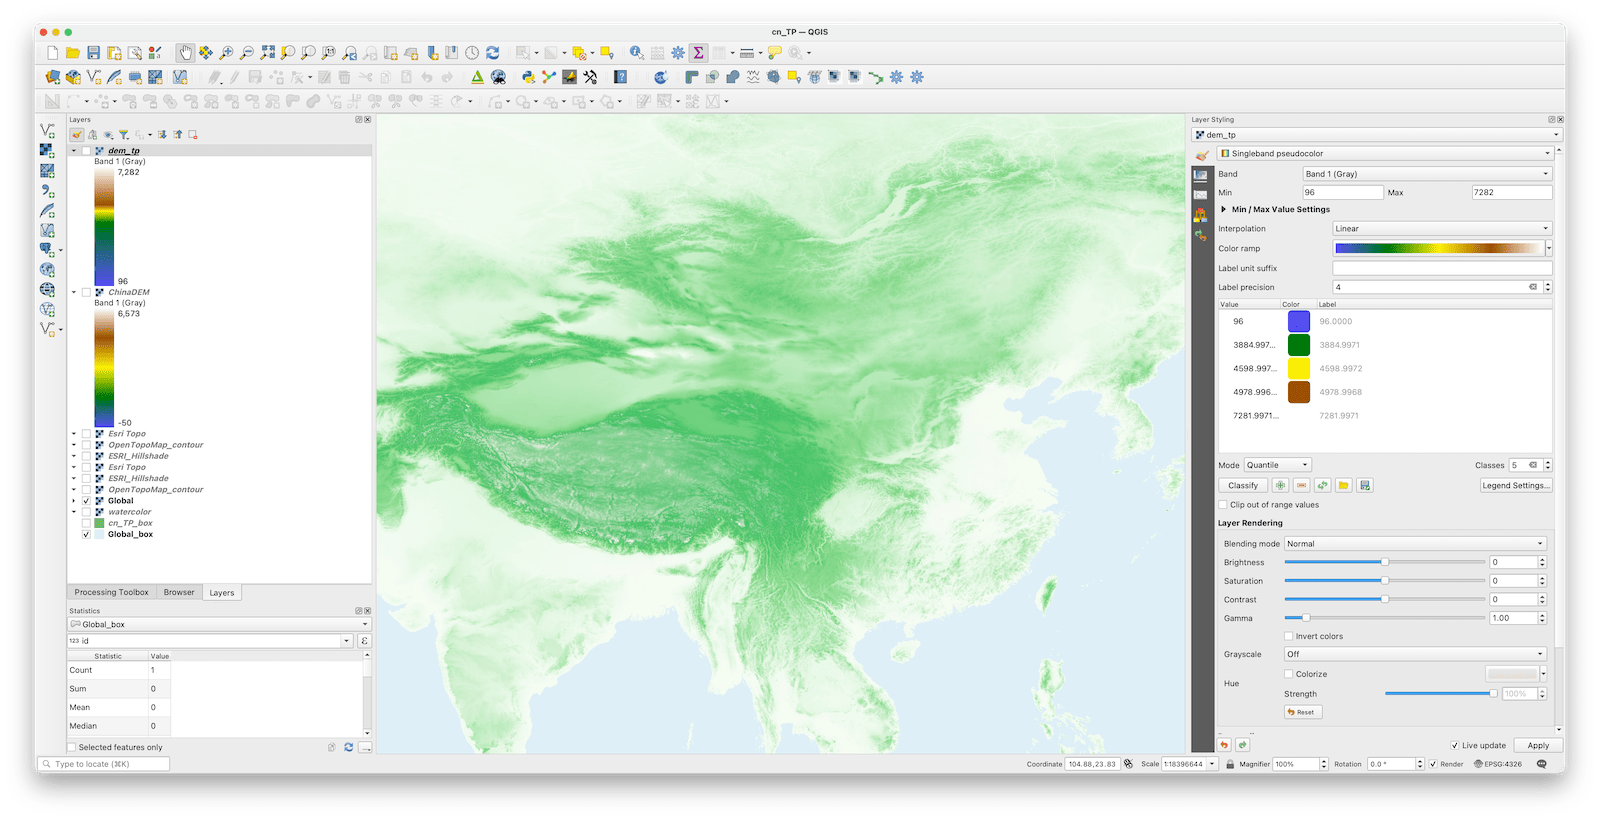
\includegraphics{Fig/skill/qgis.png}
\caption{QGIS界面}
\end{figure}

\hypertarget{ux7ed8ux56fexmind}{%
\subsection{【绘图】XMind}\label{ux7ed8ux56fexmind}}

XMind 是一款流行的思维导图软件,它帮助用户通过可视化的方式进行思维整理和知识管理。支持多种导图类型,界面友好,操作简单,且具有丰富的样式和主题,用户可以根据需要选择适合自己的导图方式和风格。此外,XMind 还支持多种文件格式,如 PDF、Excel、Word 等,方便用户进行跨平台工作和分享。。

下载地址:\url{https://xmind.cn/download/}

\begin{figure}
\centering
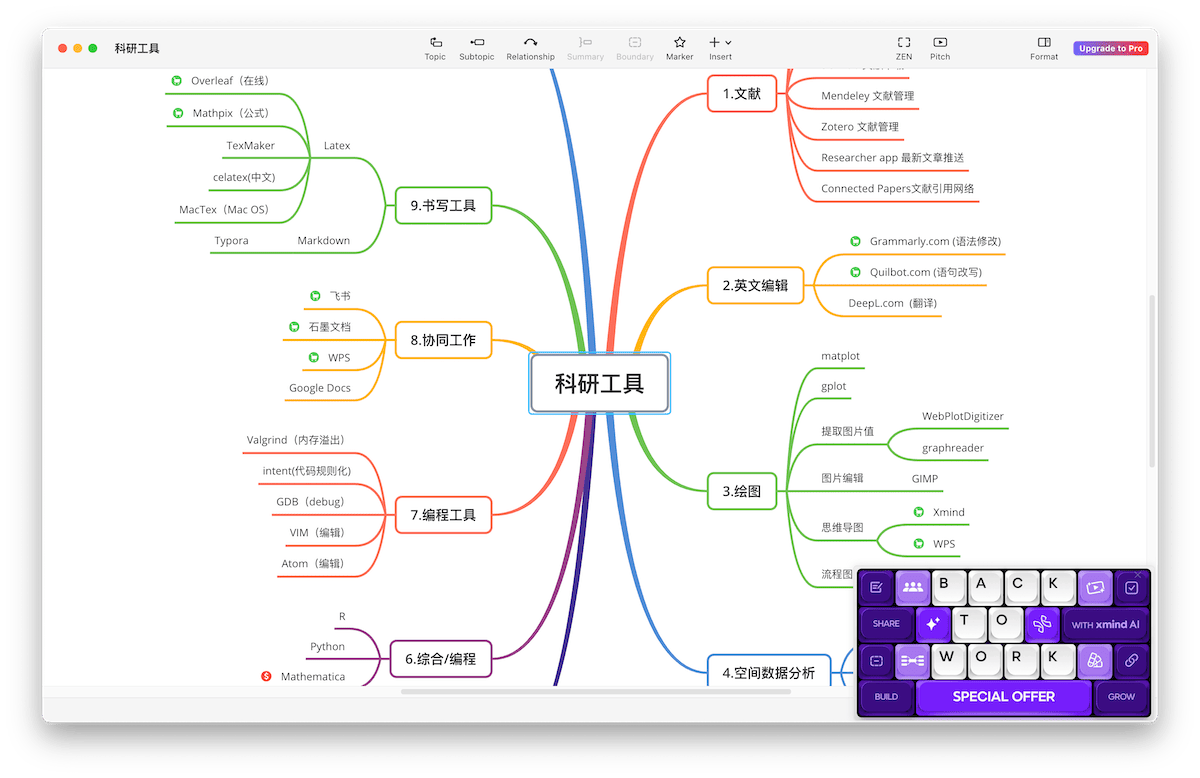
\includegraphics{Fig/skill/xmind.png}
\caption{xmind}
\end{figure}

\hypertarget{ux6587ux732emendeley-desktop}{%
\subsection{【文献】Mendeley Desktop}\label{ux6587ux732emendeley-desktop}}

Mendeley Desktop 是一款强大的文献管理软件,它帮助用户组织、整理和分享学术文献。其优势包括:支持文献的快速检索、全文搜索,以及跨平台同步;提供丰富的文献管理功能,如文献分类、标签管理、引用格式自动生成等;支持文献协作和共享,可以与同行合作整理文献,共同撰写文章。

下载地址:\url{https://www.mendeley.com/download-reference-manager}

\begin{figure}
\centering
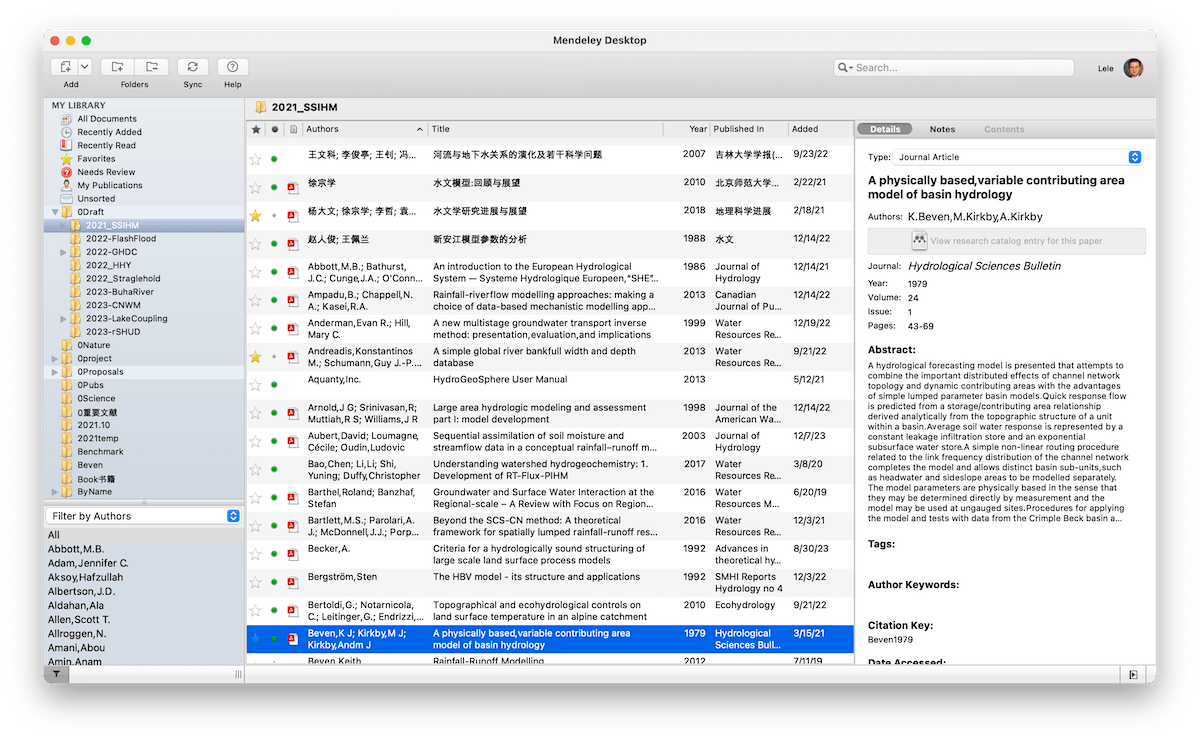
\includegraphics{Fig/skill/mendeley.png}
\caption{Mendeley desktop}
\end{figure}

\hypertarget{ux6587ux732econsensus.app}{%
\subsection{【文献】Consensus.app}\label{ux6587ux732econsensus.app}}

Consensus.app 是一个利用人工智能技术驱动的科研搜索引擎,它的核心价值在于帮助研究人员高效地查找、总结和理解大量的科学研究论文。Consensus.app 能够针对用户提出的问题,综合多篇研究论文的内容,提供一个基于研究证据的共识性回答,这对于科研工作者在进行文献综述、寻找支持自己研究假设的证据时非常有用。此外,Consensus.app 还提供了一个便捷的方式来引用相关论文,确保了答案的真实性和可靠性,从而在学术研究中发挥了重要作用。

访问地址:\url{https://Consensus.app}

\begin{figure}
\centering

\includegraphics{Fig/skill/consensus.png}
\caption{Consensus.app}
\end{figure}

\hypertarget{ux6587ux732eresearcher-app}{%
\subsection{【文献】Researcher App}\label{ux6587ux732eresearcher-app}}

Researcher App 是一个移动应用程序,旨在为研究人员提供一个便捷的方式来访问和管理科学文献。它允许用户快速搜索学术文章,阅读摘要,管理自己的引用和阅读列表,以及同步图书馆资料。Researcher App 的优势在于其用户友好的界面和实用的功能,如离线阅读、文献分享和跨平台同步,这些功能都有助于提高研究人员的工作效率。

访问地址:\url{https://www.researcher-app.com}

\begin{figure}
\centering
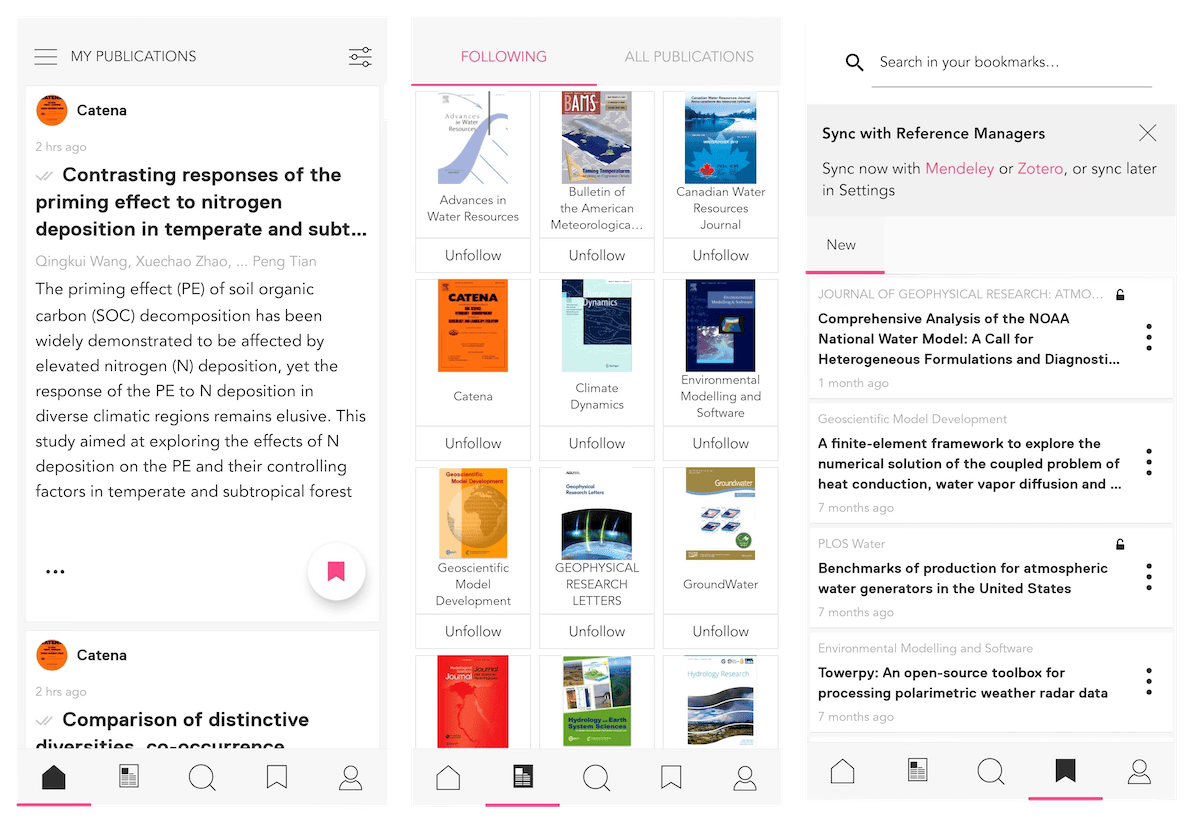
\includegraphics{Fig/skill/researcherapp.png}
\caption{researcherapp手机截屏}
\end{figure}

\hypertarget{ux6587ux732epublish-or-perish-pop}{%
\subsection{【文献】Publish or Perish (PoP)}\label{ux6587ux732epublish-or-perish-pop}}

Publish or Perish (PoP) 是一款广受学术界欢迎的科研评价工具,由Google工程师Timothy original所开发。该软件的宗旨是帮助科研工作者更有效地管理和评估他们的学术成果。Publish or Perish的主要功能包括:
1. \textbf{学术成果分析}:它可以分析学者在Google Scholar上的引用情况,提供关于其研究成果的即时反馈。
2. \textbf{引用排名}:PoP能够显示个人或机构的引用排名,以及他们在特定学科领域的表现。
3. \textbf{趋势分析}:通过分析引用数据,PoP可以帮助用户了解特定研究主题或领域的趋势和动向。
4. \textbf{成果比较}:用户可以比较不同研究者或论文的引用情况,从而对学术成就进行量化评估。
尽管Publish or Perish是一个免费软件,但用户需要意识到,它所依赖的数据源------Google Scholar------可能会受到搜索引擎算法更新的影响,从而影响评价结果的准确性和时效性。因此,虽然PoP是一个有用的工具,但它应该与其他评价方法结合使用,以获得更全面的学术评价。

\begin{figure}
\centering
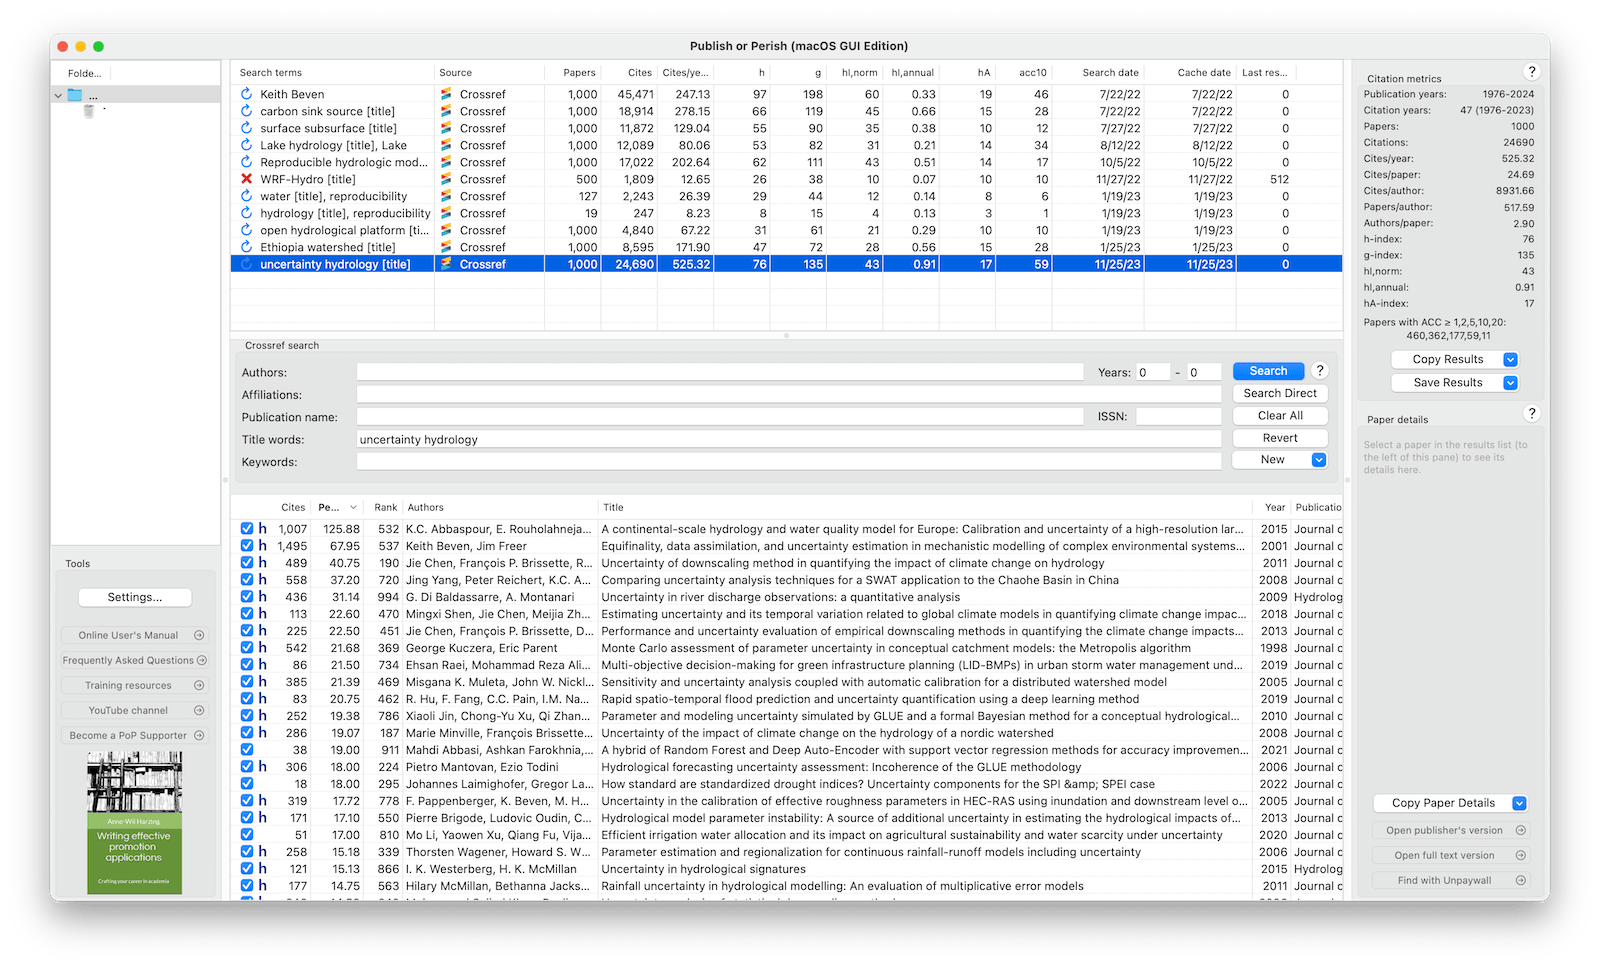
\includegraphics{Fig/skill/pop.png}
\caption{pop}
\end{figure}

\hypertarget{aiux53cachatgpt}{%
\section{AI及ChatGPT}\label{aiux53cachatgpt}}

当从事科学研究时,使用AI或大语言模型(LLM)可以作为辅助工具提供帮助和灵感。
但以下是一些建议:

\begin{itemize}
\tightlist
\item
  \textbf{准备好问题}:确保你有清晰的问题或概念,以便从LLM中获得有用的回答。明确你想要什么样的帮助,这样LLM才能更好地回应你的需求。
\item
  **验证信息:LLM提供的答案可能不总是准确或可靠的,所以记得验证这些信息。进行进一步的研究和检查,确保你得到的结果是可信的。
\item
  \textbf{适度使用}:LLM是一个很有用的工具,但也有一些局限。明确LLM的作用,将其作为辅助手段,而不是替代你自己的研究工作。
\item
  \textbf{避免偏见}:LLM模型的训练数据是从互联网上收集的,这可能包含了偏见或不准确的信息。所以在使用LLM的结果时,要保持谨慎,注意避免偏见。
\item
  \textbf{不断训练改进}:利用LLM与其他研究人员进行交流,共享反馈和经验,这样可以帮助改进和训练LLM,提高它在科研任务中的效果。
\end{itemize}

需要注意的是,尽管LLM可以为科学研究提供一些有价值的帮助,但它仍然是一个语言模型,并不能替代严格的实验设计和科学方法。将LLM作为辅助工具,与自己的专业知识和判断相结合,才能更好地实现科研任务的目标。

\hypertarget{chatgpt}{%
\subsection{ChatGPT}\label{chatgpt}}

\url{http://chat.openai.com}

\hypertarget{ux57faux4e8eapiux7684ux79c1ux6709chat-gpt3.5-ux548cgpt-4}{%
\subsubsection{基于API的私有Chat GPT3.5 和GPT-4}\label{ux57faux4e8eapiux7684ux79c1ux6709chat-gpt3.5-ux548cgpt-4}}

学术GPT部署:
\url{https://github.com/binary-husky/gpt_academic}

\hypertarget{ux667aux8c31ux6e05ux8a00}{%
\subsection{智谱清言}\label{ux667aux8c31ux6e05ux8a00}}

\url{https://chatglm.cn}

\hypertarget{ux79c1ux6709ux5927ux6a21ux578b}{%
\subsection{私有大模型}\label{ux79c1ux6709ux5927ux6a21ux578b}}

\begin{itemize}
\item
  ollama: \url{https://ollama.ai}。 Ollama 是一个开源的大型语言模型服务工具,它提供了类似 OpenAI 的 API 接口和聊天界面,使得用户能够方便地部署和使用最新版本的 GPT 模型
\item
  llama2 \url{https://github.com/facebookresearch/llama} Llama2 是由 Meta 公司开发的开源大语言模型,它在多个基准测试上取得了超越现有开源模型的成绩,具有优秀的多轮对话能力和安全性。
\item
  ChatGLM3 \url{https://github.com/THUDM/ChatGLM3}。ChatGLM3 是由智谱 AI 公司和清华大学 KEG 实验室联合发布的新一代对话预训练模型。它是基于 GLM-3 模型开发的,具有出色的多轮对话能力和良好的上下文理解能力。ChatGLM3 模型在多种场景下都表现出了优秀的性能,例如客服、教育、娱乐等。它还支持多种语言的交互,能够满足不同用户的需求。
\item
  通义千问(Qwen) \url{https://github.com/QwenLM/Qwen}。通义千问(Qwen)是阿里巴巴开源的大型语言模型,旨在实现通用人工智能(AGI),具备强大的语言处理能力和多模态交互能力,适用于多种下游任务和领域。
\end{itemize}

\hypertarget{ssh}{%
\section{ssh远程登录}\label{ssh}}

ssh是默认的远程服务器访问软件,小巧、安全、快速。
命令一般执行方式如下:

\begin{verbatim}
ssh [username@remotehost]
\end{verbatim}

第一次登录要求在本地保存登陆指纹,输入y确认。然后屏幕提示输入远程的登录密码。

其他登录参数:

\begin{itemize}
\tightlist
\item
  \textbf{-p 22} - 采用22端口登录。ssh的默认端口是22。
\item
  \textbf{-Y} - 启用远程GUI
\item
  \textbf{-i {[}file{]}} - 使用指定的登录密钥
\end{itemize}

Windows平台登录时可使用PowerShell;但是Windows平台推荐使用\href{https://mobaxterm.mobatek.net}{MobaXTerm}软件。

在Linux或者mac平台可以直接使用terminal命令行;Mac平台也推荐使用\href{https://iterm2.com}{iTerm2},可以使用多开方式。

ssh同时支持文件传输,例如sshfs和sftp。 快速的文件传输和查看,在Mac和Linux平台,可以使用\href{https://cyberduck.io}{CyberDuck}; Windows平台推荐使用\href{https://winscp.net}{WinSCP}。

\hypertarget{ux514dux5bc6ux7801ux767bux5f55}{%
\subsection{免密码登录}\label{ux514dux5bc6ux7801ux767bux5f55}}

执行ssh-keygen,可在客户端生成用户密码,生成的用户密码可于免密码的SSH登录。

\begin{verbatim}
ssh-keygen
\end{verbatim}

然后执行查看命令,查看密码申请状况。

\begin{verbatim}
ls ~/.ssh/
cat ~/.ssh/id_rsa
\end{verbatim}

将本地生成的密钥拷贝到远程服务器上,此处需要输入登陆远程服务器的密码。

\begin{verbatim}
ssh-copy-id [username@remotehost]
\end{verbatim}

如果远程服务器端口为32099,则命令改为:

\begin{verbatim}
ssh-copy-id -p 32099 [username@remotehost]
\end{verbatim}

成功之后,可以SSH免密方式登陆远程服务器。

\begin{verbatim}
ssh -i ~/.ssh/id_rsa [username@remotehost]
\end{verbatim}

如端口变为32099,则命令为:

\begin{verbatim}
ssh -p 32099 -i ~/.ssh/id_rsa [username@remotehost]
\end{verbatim}

\hypertarget{wgetux6279ux91cfux4e0bux8f7dux6570ux636e}{%
\section{wget批量下载数据}\label{wgetux6279ux91cfux4e0bux8f7dux6570ux636e}}

关于批量下载数据,请参考博客文章: \url{https://www.shulele.net/zh/eosdata/}。

\hypertarget{linux}{%
\section{Linux操作系统}\label{linux}}

\hypertarget{linux-user}{%
\subsection{用户名管理}\label{linux-user}}

新建用户\texttt{userx}

\begin{verbatim}
sudo useradd -s /bin/bash -d /home/userx/ -m -G sudo userx
\end{verbatim}

/bin/bash 是用户默认的登录shell界面。
/home/userx/ 使用户的Home目录位置。
-G sudo 是指定用户的所属的组。sudo组用户则在输入\texttt{sudo}命令时的具有root权限。

登录指定用户\texttt{userx}

\begin{verbatim}
su  userx
\end{verbatim}

\hypertarget{linuxux5e38ux7528ux7684ux547dux4ee4}{%
\subsection{Linux常用的命令。}\label{linuxux5e38ux7528ux7684ux547dux4ee4}}

\emph{部分命令的默认ubuntu系统中不存在时,需要使用apt安装。}

\begin{itemize}
\tightlist
\item
  安装软件apt: \texttt{sudo\ apt\ install\ tree}
\item
  man:使用man ls则可以查看ls命令的使用说明;man命令组合可以看所有命令的说明。
\item
  cd:切换不同的目录
\item
  ls查看目录和文件
\item
  cat 在屏幕打印出文本文件
\item
  more, head, tail,查看文本文件
\item
  tree 查看目录树结构
\item
  ip a: 查看服务器IP信息
\item
  lsblk:查看硬件设备
\item
  df: 查看磁盘设备挂载情况
\item
  du: 查看磁盘使用率
\item
  jobs: 查看后台运行的用户程序
\item
  ps:查看进程
\item
  kill: 杀死/关闭某一个进程
\item
  scp:通过ssh通道拷贝数据
\item
  rsync: 使用数据更新方式拷贝数据,支持本地数据拷贝或者远程ssh数据拷贝。
\item
  wget/curl: 数据下载
\item
  mount/umount:挂载和卸载磁盘。
\item
  grep正则表达式,用于查找文件里符合条件的字符串。
\item
  find:用于查找目录中的文件
\end{itemize}

\hypertarget{r}{%
\section{R语言}\label{r}}

R是高效且灵活的编程语言,可以高效的完成数据读写、统计分析、空间数据处理处理、并行计算等任务。

R语言是一种免费的、开源的数据分析和统计建模语言,相对于其他统计分析软件,R语言有以下显著优势:

\begin{itemize}
\item
  免费且开源:R语言是一款完全免费、开源的软件,用户可以自由地下载、使用和修改它。这使得R语言成为许多研究人员、学生和行业专业人士的首选工具之一。
\item
  具有强大的统计分析能力:R语言提供了许多统计分析和建模的方法,包括线性回归、非线性回归、时间序列分析、聚类分析、因子分析和机器学习等。R语言还提供了许多常用的数据处理和可视化工具,如数据清洗、数据可视化和报告生成等。
\item
  社区支持:R语言拥有一个庞大的用户社区,用户可以通过该社区获得技术支持、交流使用经验和分享资源等。R语言社区提供了大量的免费学习资源,包括教程、示例代码和数据集等。
\item
  可扩展性:R语言可以通过许多扩展包(packages)来扩展其功能。这些扩展包提供了各种各样的功能,从数据可视化到高级统计分析和机器学习。
\item
  易于学习和使用:R语言拥有易于学习和使用的语法和语言结构,许多人认为R语言比其他统计分析软件更加容易学习和使用。
\item
  跨平台支持:R语言可以在Windows、MacOS、Linux等多个操作系统上运行,并提供相应的安装程序和二进制文件。
\end{itemize}

本研究组的rSHUD(\url{https://github.com/shud-System/rshud}), AutoSHUD(\url{https://github.com/shud-System/autoshud})和全球数据云平台(\url{https://ghdc.ac.cn})都由R语言实现。

具体的R语言教程请参考《\href{https://www.shud.xyz/bookr/}{R在地球科学中的应用}》\url{https://www.shud.xyz/bookr/}。

\hypertarget{rstudio-server}{%
\subsection{Rstudio Server}\label{rstudio-server}}

Rstudio Server服务入口,请使用超算的账户登录。

\begin{itemize}
\tightlist
\item
  SHUDHPC: \url{https://rstudio.shud.vip} 或者 \url{http://210.77.77.22:8787}
\end{itemize}

Rstudio Server的使用手册:\url{https://s3.amazonaws.com/rstudio-server/rstudio-server-pro-0.98.507-admin-guide.pdf}

\hypertarget{python}{%
\section{Python工作环境}\label{python}}

SHUD-HPC的Python入口:\url{https://py.shud.vip}

\hypertarget{Ack}{%
\chapter{致谢}\label{Ack}}

本书一边摸索,一边完善,都是我和组内成员一起努力的成果。

\textbf{感谢我的导师,给了我探索的自由。}

\textbf{感谢我的学生,给了我继续探索的动力。}

\textbf{现有成员}

\begin{longtable}[]{@{}
  >{\raggedright\arraybackslash}p{(\columnwidth - 8\tabcolsep) * \real{0.1429}}
  >{\raggedright\arraybackslash}p{(\columnwidth - 8\tabcolsep) * \real{0.1786}}
  >{\raggedright\arraybackslash}p{(\columnwidth - 8\tabcolsep) * \real{0.2857}}
  >{\raggedright\arraybackslash}p{(\columnwidth - 8\tabcolsep) * \real{0.1429}}
  >{\raggedright\arraybackslash}p{(\columnwidth - 8\tabcolsep) * \real{0.2500}}@{}}
\toprule\noalign{}
\begin{minipage}[b]{\linewidth}\raggedright
姓名
\end{minipage} & \begin{minipage}[b]{\linewidth}\raggedright
角色
\end{minipage} & \begin{minipage}[b]{\linewidth}\raggedright
研究方向
\end{minipage} & \begin{minipage}[b]{\linewidth}\raggedright
入组时间
\end{minipage} & \begin{minipage}[b]{\linewidth}\raggedright
背景
\end{minipage} \\
\midrule\noalign{}
\endhead
\bottomrule\noalign{}
\endlastfoot
卜婷玮 & 硕士生 & 黄河源区水文变化 & 2021.09 & 西南交通大学;环境工程 \\
赵晨 & 硕士生 & 洪水预报 & 2022.10 & 兰州理工大学保送;土木工程 \\
赖吉 & 硕士生(联培) & 古气候与湖泊水文 & 2023.10 & 兰州大学;导师:李国强 \\
\end{longtable}

\textbf{曾经成员}

\begin{longtable}[]{@{}
  >{\raggedright\arraybackslash}p{(\columnwidth - 8\tabcolsep) * \real{0.1429}}
  >{\raggedright\arraybackslash}p{(\columnwidth - 8\tabcolsep) * \real{0.1786}}
  >{\raggedright\arraybackslash}p{(\columnwidth - 8\tabcolsep) * \real{0.2857}}
  >{\raggedright\arraybackslash}p{(\columnwidth - 8\tabcolsep) * \real{0.1429}}
  >{\raggedright\arraybackslash}p{(\columnwidth - 8\tabcolsep) * \real{0.2500}}@{}}
\toprule\noalign{}
\begin{minipage}[b]{\linewidth}\raggedright
姓名
\end{minipage} & \begin{minipage}[b]{\linewidth}\raggedright
角色
\end{minipage} & \begin{minipage}[b]{\linewidth}\raggedright
研究方向
\end{minipage} & \begin{minipage}[b]{\linewidth}\raggedright
入组时间
\end{minipage} & \begin{minipage}[b]{\linewidth}\raggedright
离开时间
\end{minipage} \\
\midrule\noalign{}
\endhead
\bottomrule\noalign{}
\endlastfoot
郭家乐 & 研究助理(本科) & 全球流域分级算法 & 2021.10 & 2022.06 \\
甘亚斌 & 硕士生(联培) & 未定 & 2021.01 & 2021.03 \\
邱心叶 & 硕士生(联培) & 晚第四纪干旱区生态水文过程 & 2022.10 & 兰州大学; 导师:李国强 \\
\end{longtable}

  \bibliography{book.bib,packages.bib}

\end{document}
